% =============================================================================
% Cortex Tokenomics: A Game-Theoretic Framework for Sustainable Value Accrual
% in Autonomous Agent Economies
%
% Author: Chaos Oracle, PURECORTEX Research
% =============================================================================
\documentclass[11pt,letterpaper]{article}

% --- Packages ----------------------------------------------------------------
\usepackage{amsmath,amssymb,amsthm}
\usepackage{graphicx}
\usepackage[colorlinks=true,linkcolor=blue!60!black,citecolor=green!50!black,urlcolor=blue!70!black]{hyperref}
\usepackage{booktabs}
\usepackage{float}
\usepackage[ruled,vlined,linesnumbered]{algorithm2e}
\usepackage[numbers,sort&compress]{natbib}
\usepackage[margin=1in]{geometry}
\usepackage{xcolor}
\usepackage{tikz}
\usepackage{pgfplots}
\pgfplotsset{compat=1.18}
\usetikzlibrary{arrows.meta,positioning,calc,shapes.geometric,decorations.pathmorphing}

% --- Theorem environments ----------------------------------------------------
\newtheorem{theorem}{Theorem}[section]
\newtheorem{lemma}[theorem]{Lemma}
\newtheorem{proposition}[theorem]{Proposition}
\newtheorem{corollary}[theorem]{Corollary}
\theoremstyle{definition}
\newtheorem{definition}[theorem]{Definition}
\theoremstyle{remark}
\newtheorem{remark}[theorem]{Remark}

% --- Custom commands ----------------------------------------------------------
\newcommand{\CORTEX}{\textsc{cortex}}
\newcommand{\veCORTEX}{\textsc{veCortex}}
\newcommand{\R}{\mathbb{R}}
\newcommand{\N}{\mathbb{N}}
\newcommand{\E}{\mathbb{E}}
\newcommand{\Var}{\mathrm{Var}}
\DeclareMathOperator*{\argmax}{arg\,max}
\DeclareMathOperator*{\argmin}{arg\,min}

% --- Title --------------------------------------------------------------------
\title{\textbf{Cortex Tokenomics: A Game-Theoretic Framework for\\
Sustainable Value Accrual in Autonomous Agent Economies}}
\author{Chaos Oracle\\
\textit{PURECORTEX Research}\\
\texttt{research@purecortex.io}}
\date{March 2026}

% ==============================================================================
\begin{document}

\maketitle

% --- Abstract -----------------------------------------------------------------
\begin{abstract}
We present a comprehensive tokenomic framework for \emph{PURECORTEX}, an
autonomous agent economy built on the Algorand blockchain. The framework
comprises six interlocking pillars: (i)~quadratic bonding curve graduation
with creator vesting, (ii)~volatility-adaptive dynamic fees,
(iii)~vote-escrowed staking (\veCORTEX{}) with day-one launch parity,
(iv)~protocol-level buyback-and-burn mechanics, (v)~composability rewards
via cross-agent tool invocation, and (vi)~sovereign on-chain governance
anchored by a constitutional AI Senator. We derive closed-form expressions
for bonding curve cost, dynamic fee revenue, staking yield, and deflationary
crossover conditions. Game-theoretic analysis demonstrates that the mechanism
admits a unique Nash equilibrium in which rational agents stake rather than
sell, creators commit to long-horizon vesting, and governance delegation is
individually rational when information acquisition costs exceed voting costs.
Monte Carlo simulations across 1{,}000 trajectories per scenario confirm a
deflationary crossover at approximately month~18--24, staker yields in the
15--40\% APR range, and superlinear network value growth consistent with
Metcalfe's law. A 14-dimension comparative analysis against existing agent
tokenization platforms reveals structural advantages across creator
incentives, fee adaptation, composability, and governance. The full
constitutional text, contract ABIs, and simulation methodology are provided
in the appendices.
\end{abstract}

\tableofcontents
\newpage

% --- Sections -----------------------------------------------------------------
% =============================================================================
\section{Introduction}
\label{sec:introduction}
% =============================================================================

The emergence of large language models and autonomous AI agents has catalyzed a
paradigm shift in decentralized infrastructure. Where blockchains once served
primarily as ledgers for value transfer and smart contract execution, they now
function as \emph{coordination substrates} for economically sovereign AI
agents---entities capable of invoking tools, managing treasuries, and
transacting with both humans and other agents without centralized intermediation.
This transformation demands tokenomic architectures purpose-built for agent
economies, yet the prevailing designs inherit assumptions from human-centric
decentralized finance (DeFi) that fail under the distinct incentive landscape of
autonomous actors.

\subsection{Motivation}
\label{subsec:motivation}

An AI agent operating within an on-chain economy requires infrastructure that
simultaneously satisfies five desiderata:

\begin{enumerate}
  \item \textbf{Capital formation.} Agents must raise initial capital through
    mechanisms that price discovery fairly and reward early supporters without
    enabling manipulative extraction.
  \item \textbf{Revenue sustainability.} The protocol must generate fee revenue
    that adapts to market conditions, ensuring solvency during low-activity
    periods without extracting punitive rents during calm markets.
  \item \textbf{Stakeholder alignment.} Creators, stakers, users, and the
    protocol treasury must share revenue in proportions that sustain
    participation across all roles.
  \item \textbf{Composability.} Agents must be able to invoke one another's
    capabilities (tools, data feeds, inference endpoints) through standardized
    protocols, with economic incentives that reward interoperability.
  \item \textbf{Governance.} Protocol parameters, treasury allocations, and
    constitutional norms must be governable by stakeholders, with safeguards
    against both capture and ossification.
\end{enumerate}

\subsection{Problem Statement}
\label{subsec:problem}

Existing agent tokenization platforms exhibit five structural deficiencies that
undermine long-term ecosystem health:

\begin{description}
  \item[P1: No creator vesting.] Creators receive their full token allocation at
    launch, enabling immediate liquidation. This misaligns creator incentives
    with long-term agent development and facilitates pump-and-dump dynamics
    wherein creators abandon agents after extracting initial liquidity.

  \item[P2: Post-hoc staking disadvantage.] When staking mechanisms are
    introduced after token launch, early adopters who provided initial liquidity
    and bore maximum risk receive no preferential treatment. Late entrants
    capture identical yields despite contributing no price-discovery capital.

  \item[P3: Flat fee structures.] A fixed percentage trading fee (e.g., 1\%)
    fails to adapt to volatility regimes. During high-volatility periods, flat
    fees are insufficient to compensate liquidity providers for adverse
    selection; during low-volatility periods, they impose unnecessary friction
    that suppresses trading volume.

  \item[P4: Agent silos.] Without standardized inter-agent communication
    protocols and economic incentives for composability, each agent operates as
    an isolated service. This prevents the emergence of compound agent
    workflows---multi-agent pipelines where specialized agents collaborate on
    complex tasks.

  \item[P5: No on-chain governance.] Protocol parameters are controlled by
    centralized teams with no formal governance mechanism, no constitutional
    framework, and no stakeholder recourse. This introduces platform risk and
    regulatory uncertainty.
\end{description}

\subsection{Contributions}
\label{subsec:contributions}

We present a six-pillar tokenomic framework that addresses each deficiency:

\begin{enumerate}
  \item \textbf{Bonding curve graduation with creator vesting}
    (Section~\ref{sec:bonding-curve}). A quadratic bonding curve provides
    transparent price discovery during agent launch, with mandatory 180-day
    creator vesting that releases 1\% immediately and the remainder linearly.
    Upon reaching a graduation threshold, liquidity atomically migrates to a
    decentralized exchange with a 10-year LP lock.

  \item \textbf{Volatility-adaptive dynamic fees}
    (Section~\ref{sec:dynamic-fees}). A continuous fee function maps realized
    volatility to trading fees in the range $[0.5\%, 2.0\%]$, with a five-way
    revenue split among stakers, creators, treasury, referrers, and
    composability rewards.

  \item \textbf{Vote-escrowed staking} (Section~\ref{sec:vecortex-staking}).
    The \veCORTEX{} mechanism, available from day one of platform launch,
    grants governance weight and revenue share proportional to both the quantity
    staked and the lock duration, with a maximum four-year commitment.

  \item \textbf{Protocol-level buyback-and-burn}
    (Section~\ref{sec:buyback-burn}). Multiple revenue streams fund a weekly
    buyback with a supply-proportional cap, establishing conditions under which
    the token supply becomes net deflationary.

  \item \textbf{Composability rewards} (Section~\ref{sec:composability}).
    Cross-agent tool invocation via the Model Context Protocol (MCP) generates
    micropayment flows with a composability tax, and a Composability Score
    distributes weekly rewards to the most-integrated agents.

  \item \textbf{Sovereign on-chain governance}
    (Section~\ref{sec:governance}). A constitutional governance framework
    features a protocol-owned AI Senator that proposes but cannot vote,
    \veCORTEX{}-weighted Lawmaker Agents with liquid delegation, and a
    multi-tiered proposal lifecycle anchored by an on-chain constitution.
\end{enumerate}

We provide formal game-theoretic analysis (Section~\ref{sec:game-theory})
demonstrating that the mechanism admits equilibria aligned with ecosystem
health, Monte Carlo simulations (Section~\ref{sec:simulations}) validating
quantitative predictions, security analysis (Section~\ref{sec:security}), and a
14-dimension comparative analysis (Section~\ref{sec:comparative}) against
existing platforms.

\subsection{Paper Organization}
\label{subsec:organization}

Section~\ref{sec:related-work} surveys related work in bonding curves,
vote-escrowed tokenomics, agent tokenization, and game-theoretic mechanism
design. Section~\ref{sec:architecture} presents the overall token architecture,
allocation, and vesting schedules. Sections~\ref{sec:bonding-curve}
through~\ref{sec:governance} detail each of the six pillars. Section~\ref{sec:game-theory}
provides formal game-theoretic analysis. Section~\ref{sec:simulations} presents
simulation results. Section~\ref{sec:security} addresses security
considerations. Section~\ref{sec:comparative} provides comparative analysis.
Section~\ref{sec:conclusion} concludes. The appendices contain full proofs
(Appendix~\ref{app:proofs}), simulation methodology
(Appendix~\ref{app:simulation}), contract ABIs
(Appendix~\ref{app:contracts}), and the full constitutional text
(Appendix~\ref{app:constitution}).

% =============================================================================
\section{Related Work}
\label{sec:related-work}
% =============================================================================

This section surveys four streams of literature that inform the PURECORTEX
tokenomic design: bonding curves and automated market makers, vote-escrowed
tokenomics, agent tokenization platforms, and game-theoretic mechanism design
for decentralized systems.

\subsection{Bonding Curves and Continuous Token Models}
\label{subsec:rw-bonding}

The concept of automated price discovery through mathematical functions
originates with Hanson's logarithmic market scoring rule for prediction
markets~\citep{hanson2003combinatorial}. Hanson demonstrated that a cost
function derived from a convex potential can simultaneously serve as a market
maker and an information aggregation device. The Bancor protocol generalized
this insight to arbitrary token issuance, introducing continuous liquidity
through a reserve-backed bonding curve parameterized by a connector
weight~\citep{bancor2017}. Subsequent work by Angeris et
al.~\citep{angeris2020improved} provided rigorous analysis of constant-product
market makers (the Uniswap model), establishing conditions under which
arbitrageurs drive prices toward external reference values.

Our quadratic bonding curve (Section~\ref{sec:bonding-curve}) builds on this
lineage but introduces two innovations absent from prior work: a deterministic
graduation mechanism that atomically transitions liquidity from the bonding
curve to a decentralized exchange, and a mandatory creator vesting schedule
that conditions token release on elapsed time rather than price milestones.

\subsection{Vote-Escrowed Tokenomics}
\label{subsec:rw-ve}

The vote-escrowed (ve) model was pioneered by Curve Finance's
veCRV~\citep{curvefinance2020, egorov2019stableswap}, wherein users lock CRV
tokens for up to four years to receive governance weight proportional to the
remaining lock duration. This mechanism simultaneously reduces circulating
supply, aligns governance power with long-term commitment, and distributes
protocol revenue to lockers. Balancer subsequently adapted the model as
veBAL~\citep{balancer2022vebal}, adding a gauge-based emission allocation
system.

Two limitations of existing ve implementations motivate our design. First,
veCRV was introduced approximately two years after CRV launch, disadvantaging
early participants who could not lock tokens from inception. Second, the linear
decay of governance weight creates a ``cliff problem'' wherein users must
repeatedly re-lock to maintain influence, introducing gas costs and
attentional overhead. The \veCORTEX{} mechanism
(Section~\ref{sec:vecortex-staking}) addresses the first limitation by
launching contemporaneously with the token, and mitigates the second through a
boost multiplier that rewards sustained participation.

\subsection{Agent Tokenization Platforms}
\label{subsec:rw-agent}

The tokenization of AI agents---the process of creating tradeable digital
assets representing ownership stakes in or usage rights to autonomous
agents---has emerged as a distinct category within decentralized infrastructure.
The most prominent exemplar, which we refer to as \emph{Platform~A} for
neutrality, implements the following design:

\begin{itemize}
  \item A fixed supply of $10^9$ tokens per agent, with 1\% allocated to the
    creator at launch and no vesting schedule.
  \item A flat 1\% trading fee on all buy and sell transactions, split between
    the creator and the protocol.
  \item Initial liquidity bootstrapped through a bonding curve, with LP tokens
    locked upon migration to a decentralized exchange.
  \item No on-chain governance mechanism; protocol parameters are controlled by
    the development team.
  \item No composability framework; agents operate as isolated services.
\end{itemize}

While Platform~A demonstrated product-market fit and catalyzed the agent token
category, its design exhibits the five structural deficiencies enumerated in
Section~\ref{subsec:problem}. The absence of creator vesting has been
empirically associated with rapid creator exits; the flat fee structure fails
to adapt to volatility regimes; and the lack of governance creates platform
risk.

\subsection{Game Theory and Mechanism Design in DeFi}
\label{subsec:rw-game-theory}

Roughgarden~\citep{roughgarden2020transaction} established a formal framework
for analyzing transaction fee mechanisms as games between users and block
producers, proving that EIP-1559-style mechanisms are incentive-compatible
under certain conditions. Daian et al.~\citep{daian2020flash} identified
miner extractable value (MEV) as a fundamental game-theoretic challenge in
decentralized exchanges, demonstrating that frontrunning and sandwich attacks
constitute rational strategies under existing fee structures.

In the broader mechanism design literature,
Myerson~\citep{myerson1981optimal} established revenue-optimal auction theory,
while Spence~\citep{spence1973job} introduced the signaling model that we
adapt in Section~\ref{sec:game-theory} to analyze bonding curve participation
as a quality signal. Zargham et al.~\citep{zargham2020} proposed cadCAD-based
simulation frameworks for economic games in token ecosystems, providing
methodological grounding for our simulation approach.

The intersection of game theory and governance has been explored in the context
of liquid democracy and delegative voting~\citep{fudenberg1991game}. Our
governance model (Section~\ref{sec:governance}) extends this literature by
introducing an AI Senator agent that participates in the proposal process but
is constitutionally prohibited from voting, creating a novel separation of
powers within a token-governed system.

\subsection{Algorand as Settlement Layer}
\label{subsec:rw-algorand}

The Algorand blockchain~\citep{algorand2019, chen2019algorand} provides
several properties that are structurally advantageous for agent tokenomics:
immediate transaction finality (no probabilistic confirmation), native asset
support through the Algorand Standard Asset (ASA) model, atomic transaction
groups that enable multi-step operations without reentrancy risk, and
LogicSig-based programmable accounts that can enforce time-locked LP
positions without trusted intermediaries.

These properties eliminate entire classes of vulnerabilities present in
EVM-based implementations (see Section~\ref{sec:security}) and enable the
atomic graduation mechanism described in Section~\ref{sec:bonding-curve}.

% =============================================================================
\section{Token Architecture}
\label{sec:architecture}
% =============================================================================

This section specifies the CORTEX token parameters, allocation structure,
vesting schedules, and smart contract architecture that form the foundation of
the PURECORTEX economy.

\subsection{Token Parameters}
\label{subsec:token-params}

Table~\ref{tab:token-params} summarizes the core token parameters.

\begin{table}[H]
\centering
\caption{CORTEX token parameters.}
\label{tab:token-params}
\begin{tabular}{@{}ll@{}}
\toprule
\textbf{Parameter} & \textbf{Value} \\
\midrule
Name & CORTEX \\
Standard & Algorand Standard Asset (ASA) \\
Total Supply & $10{,}000{,}000{,}000{,}000{,}000$ ($10^{16}$, i.e., 10 quadrillion) \\
Decimals & 6 \\
Smallest Unit & $10^{-6}$ CORTEX ($1\;\mu\text{CORTEX}$) \\
Chain & Algorand MainNet \\
Finality & Instant ($< 3.3$~s block time) \\
Transferability & Unrestricted after TGE \\
\bottomrule
\end{tabular}
\end{table}

The large total supply ($10^{16}$) with six decimal places ensures sufficient
granularity for micropayment flows in agent-to-agent transactions (see
Section~\ref{sec:composability}) while maintaining human-readable unit prices
during early-stage price discovery.

\subsection{Allocation Structure}
\label{subsec:allocation}

The total supply is partitioned into six categories as specified in
Table~\ref{tab:allocation}. The allocation reflects a community-first
philosophy: \textbf{0\% to VCs, 0\% to team/advisors} --- only a single
creator allocation of 10\%, with 90\% directed to community and ecosystem
participants.

\begin{table}[H]
\centering
\caption{CORTEX token allocation.}
\label{tab:allocation}
\begin{tabular}{@{}lrrl@{}}
\toprule
\textbf{Category} & \textbf{Percentage} & \textbf{Tokens ($\times 10^{12}$)} & \textbf{Vesting} \\
\midrule
Creator & 10\% & 1{,}000 & 10\% at TGE, 90\% daily over 180 days \\
Genesis Distribution & 31\% & 3{,}100 & Airdrop to early testnet users \& Algorand community \\
Future Emissions \& Staking & 24\% & 2{,}400 & veCORTEX rewards, 4-year halving decay \\
Liquidity & 15\% & 1{,}500 & CORTEX/ALGO DEX LP (10-year lock) + agent token LPs \\
Agent Incentives & 15\% & 1{,}500 & Graduation bonuses, composability rewards, performance \\
Assistance Fund & 5\% & 500 & Seed for buyback engine; self-sustaining from revenue \\
\midrule
\textbf{Total} & \textbf{100\%} & \textbf{10{,}000} & \\
\bottomrule
\end{tabular}
\end{table}

The Assistance Fund receives 90\% of \emph{all} protocol revenue (trading
fees, agent creation fees, x402 commissions, LP fees) and uses it to
continuously buy CORTEX from the open market and burn it. The initial 5\%
seed provides the fund with operational capital at launch; thereafter it is
entirely self-sustaining from protocol revenue. The remaining 10\% of
protocol revenue covers operations and development (see
Section~\ref{sec:dynamic-fees}).

\subsection{Vesting Formulas}
\label{subsec:vesting}

We define three distinct vesting schedules, each with a closed-form expression.

\subsubsection{Creator Vesting}

The creator allocation ($A_c = 10\%$ of total supply) vests according to:

\begin{equation}
  V_{\text{creator}}(d) = 0.10 \cdot A_c + 0.90 \cdot A_c \cdot \frac{\min(d, 180)}{180}
  \label{eq:creator-vesting}
\end{equation}

This releases 10\% of the allocation at the Token Generation Event (enabling
the creator to provide initial liquidity and demonstrate commitment) and vests
the remaining 90\% linearly over 180 days via daily unlocks. The creator's
unvested tokens are held in a smart contract escrow; premature withdrawal
attempts revert. There is no separate team or advisor allocation --- the
creator allocation is the sole insider distribution.

\subsubsection{Staking Emissions}

The staking emission pool of $R_{\text{total}} = 2.4 \times 10^{15}$ tokens
(24\% of total supply) is distributed over a four-year period with declining
annual weights:

\begin{equation}
  E(y) = R_{\text{total}} \cdot \frac{w_y}{\sum_{i=1}^{4} w_i}
  \label{eq:staking-emission}
\end{equation}

where the weight vector is $\mathbf{w} = (0.4,\; 0.3,\; 0.2,\; 0.1)$ and $y
\in \{1,2,3,4\}$ denotes the year. This yields:

\begin{align}
  E(1) &= 2.4 \times 10^{15} \times 0.4 = 9.6 \times 10^{14} \label{eq:emission-y1} \\
  E(2) &= 2.4 \times 10^{15} \times 0.3 = 7.2 \times 10^{14} \label{eq:emission-y2} \\
  E(3) &= 2.4 \times 10^{15} \times 0.2 = 4.8 \times 10^{14} \label{eq:emission-y3} \\
  E(4) &= 2.4 \times 10^{15} \times 0.1 = 2.4 \times 10^{14} \label{eq:emission-y4}
\end{align}

The declining schedule front-loads rewards to incentivize early staking while
ensuring four full years of emission-funded yield.

\subsubsection{Genesis Distribution}

The genesis distribution of $A_{\text{gen}} = 3.1 \times 10^{15}$ tokens
(31\% of total supply) is released in full at TGE via airdrop to early testnet
participants and the Algorand community. There is no vesting schedule for this
allocation --- recipients have immediate, unrestricted access:

\begin{equation}
  V_{\text{gen}}(d) = A_{\text{gen}} \quad \forall\; d \geq 0
  \label{eq:genesis-vesting}
\end{equation}

The immediate release ensures broad distribution from day one and maximizes
the decentralization of the circulating supply at launch.

\subsection{Smart Contract Architecture}
\label{subsec:contract-arch}

The PURECORTEX protocol is implemented as a system of three interacting
Algorand smart contracts, depicted schematically in
Figure~\ref{fig:contract-arch}.

\begin{figure}[H]
\centering
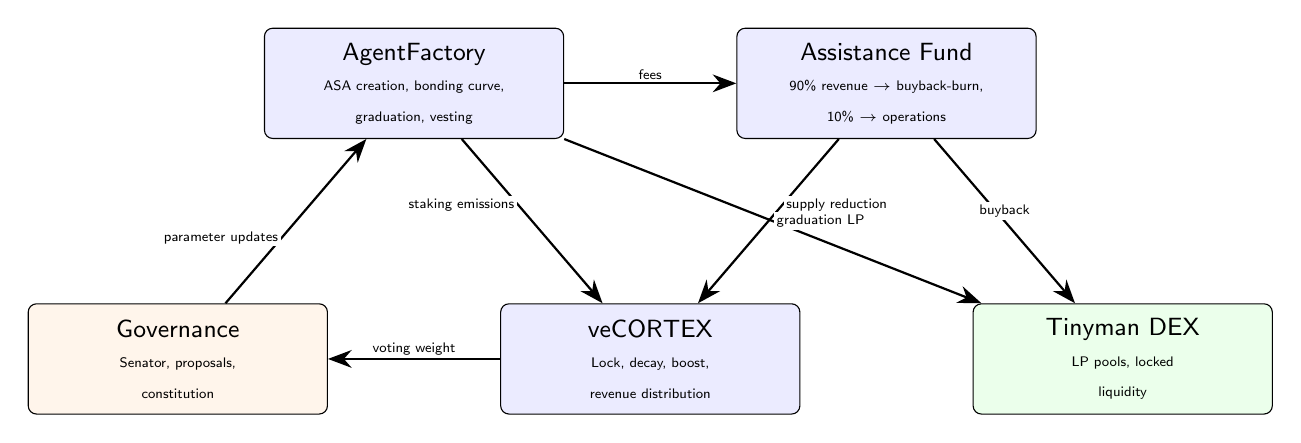
\begin{tikzpicture}[
  box/.style={draw, rounded corners=3pt, minimum width=3.8cm, minimum height=1.4cm,
              fill=blue!8, font=\small\sffamily, align=center},
  arrow/.style={-{Stealth[length=3mm]}, thick},
  label/.style={font=\tiny\sffamily, midway, fill=white, inner sep=1pt}
]
  % Nodes
  \node[box] (factory) at (0,0) {AgentFactory\\{\tiny ASA creation, bonding curve,}\\{\tiny graduation, vesting}};
  \node[box] (treasury) at (6,0) {Assistance Fund\\{\tiny 90\% revenue $\to$ buyback-burn,}\\{\tiny 10\% $\to$ operations}};
  \node[box] (ve) at (3,-3.5) {veCORTEX\\{\tiny Lock, decay, boost,}\\{\tiny revenue distribution}};
  \node[box, fill=green!8] (tinyman) at (9,-3.5) {Tinyman DEX\\{\tiny LP pools, locked}\\{\tiny liquidity}};
  \node[box, fill=orange!8] (governance) at (-3,-3.5) {Governance\\{\tiny Senator, proposals,}\\{\tiny constitution}};

  % Arrows
  \draw[arrow] (factory) -- node[label, above] {fees} (treasury);
  \draw[arrow] (treasury) -- node[label, right, pos=0.4] {supply reduction} (ve);
  \draw[arrow] (factory) -- node[label, left, pos=0.4] {staking emissions} (ve);
  \draw[arrow] (factory.south east) -- node[label, right, pos=0.5] {graduation LP} (tinyman);
  \draw[arrow] (treasury) -- node[label, above] {buyback} (tinyman);
  \draw[arrow] (ve) -- node[label, above] {voting weight} (governance);
  \draw[arrow] (governance) -- node[label, left, pos=0.4] {parameter updates} (factory);
\end{tikzpicture}
\caption{Smart contract architecture. Arrows indicate primary data and value
flows between contracts. Tinyman DEX and Governance are external to the core
protocol but interact through well-defined interfaces.}
\label{fig:contract-arch}
\end{figure}

\begin{description}
  \item[AgentFactory.] Handles agent creation, bonding curve pricing, token
    minting via ASA inner transactions, creator vesting escrow, and graduation
    (atomic LP formation on Tinyman). Stores per-agent state in Algorand box
    storage: current supply, base price, slope, graduation status, and creator
    vesting schedule.

  \item[SovereignTreasury (Assistance Fund).] Receives 90\% of all protocol
    revenue from trading fees, agent creation fees, x402 commissions, and LP
    fees. Executes continuous buyback-and-burn operations
    (Section~\ref{sec:buyback-burn}) by purchasing CORTEX from the open DEX
    market and sending it to the Algorand zero address. The remaining 10\% of
    protocol revenue is directed to an operations account for development and
    infrastructure costs. Seeded with 5\% of total supply at genesis;
    thereafter entirely self-sustaining from protocol revenue.

  \item[veCORTEX.] Manages token locking, computes time-decaying governance
    weight, and calculates boost multipliers for staking emissions. Lock state
    is stored in per-user box storage with fields for locked amount, lock
    duration, lock start timestamp, and accumulated emission rewards. Fee
    revenue no longer flows directly to stakers --- instead, stakers benefit
    from the continuous supply reduction executed by the Assistance Fund.
\end{description}

All three contracts interact through Algorand atomic transaction groups,
ensuring that multi-step operations (e.g., graduation: sell remaining bonding
curve supply, form LP pair, lock LP tokens, distribute graduation bonus) either
complete entirely or revert entirely. This atomicity eliminates the reentrancy
and partial-execution risks inherent in EVM-based designs.

% =============================================================================
\section{Bonding Curve Graduation}
\label{sec:bonding-curve}
% =============================================================================

This section formalizes the quadratic bonding curve used for agent token
issuance, derives the cost function, proves key properties, specifies the
graduation mechanism, and compares the quadratic form against alternative curve
shapes.

\subsection{Quadratic Pricing Function}
\label{subsec:pricing}

\begin{definition}[Bonding Curve Price]
\label{def:bc-price}
Let $q \geq 0$ denote the cumulative quantity of agent tokens sold. The
instantaneous price is defined by the affine function:
\begin{equation}
  P(q) = B + S \cdot q
  \label{eq:price-function}
\end{equation}
where $B > 0$ is the base price (in CORTEX per agent token) and $S > 0$ is
the slope parameter.
\end{definition}

The base price $B$ sets a nonzero floor that prevents zero-cost acquisition of
the first tokens, while the slope $S$ determines the rate at which marginal
price increases with cumulative supply. Both parameters are set at agent
creation time and are immutable thereafter.

\subsection{Cost Function}
\label{subsec:cost}

A buyer purchasing $n$ tokens when the current cumulative supply is $s$ pays
the integral of the price function over the interval $[s, s+n]$:

\begin{equation}
  C(s, n) = \int_{s}^{s+n} P(q) \, dq = \int_{s}^{s+n} (B + Sq) \, dq
  \label{eq:cost-integral}
\end{equation}

Evaluating:
\begin{align}
  C(s, n) &= \left[ Bq + \frac{S q^2}{2} \right]_{s}^{s+n} \notag \\
  &= B(s+n) + \frac{S(s+n)^2}{2} - Bs - \frac{Ss^2}{2} \notag \\
  &= Bn + \frac{S}{2}\left[(s+n)^2 - s^2\right] \notag \\
  &= Bn + \frac{S}{2}(2sn + n^2) \notag \\
  &= n \cdot B + \frac{S(2sn + n^2)}{2}
  \label{eq:cost-closed}
\end{align}

The average price per token for this purchase is:
\begin{equation}
  \bar{P}(s, n) = \frac{C(s, n)}{n} = B + S\left(s + \frac{n}{2}\right)
  \label{eq:avg-price}
\end{equation}

which equals the price at the midpoint of the interval $[s, s+n]$, a
consequence of the linearity of $P(q)$.

\subsection{Monotonicity and Convexity}
\label{subsec:monotonicity}

\begin{proposition}[Monotonicity and Convexity]
\label{prop:monotonicity}
The cost function $C(s, n)$ satisfies:
\begin{enumerate}
  \item[(i)] \textbf{Monotonicity in $s$:} For fixed $n > 0$,
    $\partial C / \partial s > 0$.
  \item[(ii)] \textbf{Monotonicity in $n$:} For fixed $s \geq 0$,
    $\partial C / \partial n > 0$.
  \item[(iii)] \textbf{Convexity in $n$:} For fixed $s \geq 0$,
    $\partial^2 C / \partial n^2 > 0$.
\end{enumerate}
\end{proposition}

\begin{proof}
From Equation~\eqref{eq:cost-closed}:
\begin{align}
  \frac{\partial C}{\partial s} &= Sn > 0 \quad \text{since } S, n > 0. \label{eq:dc-ds} \\
  \frac{\partial C}{\partial n} &= B + S(s + n) = P(s+n) > 0 \quad \text{since } B, S > 0. \label{eq:dc-dn} \\
  \frac{\partial^2 C}{\partial n^2} &= S > 0. \label{eq:d2c-dn2}
\end{align}
Properties (i)--(iii) follow directly. \qed
\end{proof}

\begin{remark}
Property (iii) implies that the marginal cost of each additional token is
strictly increasing. This creates a natural scarcity premium: later buyers
pay more per token than earlier buyers, which (a)~rewards early price
discovery and (b)~discourages large single-transaction accumulation.
\end{remark}

\subsection{Graduation Mechanism}
\label{subsec:graduation}

\begin{definition}[Graduation]
\label{def:graduation}
An agent token \emph{graduates} when its bonding curve accumulates a total of
$G$ CORTEX in proceeds, where $G = 50{,}000$ CORTEX is the graduation
threshold. At graduation, the following atomic transaction group executes:
\begin{enumerate}
  \item The bonding curve is frozen (no further buys or sells).
  \item The accumulated CORTEX and remaining agent tokens form an LP pair on
    Tinyman.
  \item The LP tokens are transferred to a LogicSig account that enforces a
    10-year lock (Section~\ref{sec:security}).
  \item A graduation bonus is distributed: 50\% to the creator, 30\% to
    early buyers (pro-rata by purchase timestamp), and 20\% is burned.
\end{enumerate}
\end{definition}

The graduation threshold $G$ is a governance-adjustable parameter
(Section~\ref{sec:governance}). The atomic execution via Algorand transaction
groups ensures that no partial state transitions can occur---either the full
graduation completes or the bonding curve remains active.

\subsubsection{LP Lock via LogicSig}

The LP tokens are sent to an Algorand LogicSig account whose compiled program
enforces:

\begin{enumerate}
  \item No transactions are permitted until $t_{\text{graduation}} + 10
    \text{ years}$ (encoded as a round number based on 3.3-second block
    times).
  \item After the lock expires, only the AgentFactory contract can initiate
    withdrawal.
  \item The LogicSig program is stateless and immutable---once deployed, its
    logic cannot be altered.
\end{enumerate}

This provides a strictly stronger guarantee than EVM-based LP locks that rely
on time-lock contracts with potential admin keys.

\subsection{Graduation Bonus Distribution}
\label{subsec:grad-bonus}

Let $G_{\text{bonus}}$ denote the graduation bonus pool (a fixed percentage of
bonding curve proceeds designated for distribution). The allocation is:

\begin{equation}
  G_{\text{bonus}} = G_{\text{creator}} + G_{\text{early}} + G_{\text{burn}}
  \label{eq:grad-bonus}
\end{equation}

with $G_{\text{creator}} = 0.5 \cdot G_{\text{bonus}}$, $G_{\text{early}} =
0.3 \cdot G_{\text{bonus}}$, and $G_{\text{burn}} = 0.2 \cdot G_{\text{bonus}}$.

Early buyer shares are computed pro-rata by inverse purchase time:
\begin{equation}
  \text{share}_i = \frac{n_i \cdot (t_{\text{grad}} - t_i)^{-1}}{\sum_j n_j \cdot (t_{\text{grad}} - t_j)^{-1}}
  \label{eq:early-share}
\end{equation}
where $n_i$ is the number of tokens purchased by buyer $i$ at time $t_i$, and
$t_{\text{grad}}$ is the graduation timestamp. This weights earlier purchases
more heavily, rewarding participants who provided initial price discovery
capital.

\subsection{Comparison of Curve Shapes}
\label{subsec:curve-comparison}

\begin{theorem}[Quadratic vs.\ Linear vs.\ Exponential Curves]
\label{thm:curve-comparison}
Consider three bonding curve families parameterized to produce identical total
cost at a reference supply $q^*$:
\begin{align}
  P_{\text{lin}}(q) &= B_1 \quad \text{(constant/linear cost)} \label{eq:linear} \\
  P_{\text{quad}}(q) &= B_2 + S_2 q \quad \text{(quadratic cost)} \label{eq:quadratic} \\
  P_{\text{exp}}(q) &= B_3 e^{\alpha q} \quad \text{(exponential cost)} \label{eq:exponential}
\end{align}
Then for any $q > q^*$:
\begin{enumerate}
  \item[(i)] The exponential curve produces the highest marginal price:
    $P_{\text{exp}}(q) > P_{\text{quad}}(q) > P_{\text{lin}}(q)$.
  \item[(ii)] The quadratic curve maximizes the ratio of early-buyer surplus
    to late-buyer cost:
    \begin{equation}
      \frac{P_{\text{quad}}(q^*) - P_{\text{quad}}(0)}{P_{\text{quad}}(q) - P_{\text{quad}}(q^*)}
      > \frac{P_{\text{exp}}(q^*) - P_{\text{exp}}(0)}{P_{\text{exp}}(q) - P_{\text{exp}}(q^*)}
      \label{eq:surplus-ratio}
    \end{equation}
    for sufficiently large $q$.
  \item[(iii)] The quadratic curve uniquely satisfies both
    \emph{accessibility} (finite cost at all $q$) and
    \emph{scarcity} ($P'(q) > 0$, $P''(q) = 0$, linear price growth).
\end{enumerate}
\end{theorem}

The proof is provided in Appendix~\ref{app:proofs}. The key insight is that
the quadratic curve (linear price) occupies a Goldilocks position: it provides
meaningful scarcity premium (unlike the flat curve) without the explosive price
growth that makes the exponential curve inaccessible to later participants
(which concentrates value among insiders and reduces long-term liquidity depth).

\begin{figure}[H]
\centering
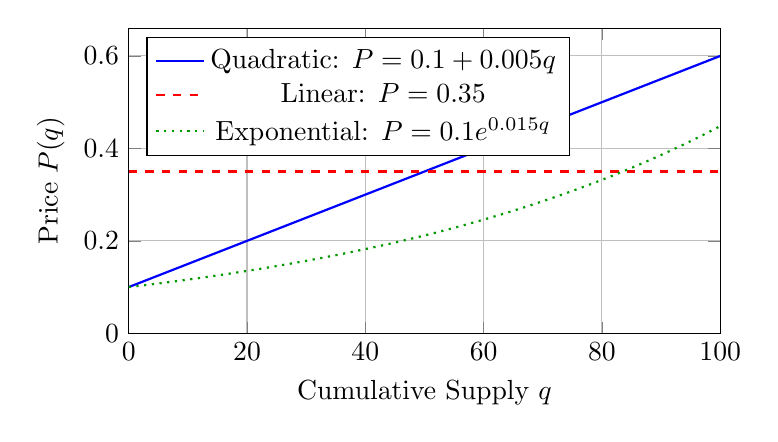
\begin{tikzpicture}
\begin{axis}[
  width=0.75\textwidth, height=0.45\textwidth,
  xlabel={Cumulative Supply $q$},
  ylabel={Price $P(q)$},
  legend pos=north west,
  grid=major,
  xmin=0, xmax=100,
  ymin=0,
]
\addplot[blue, thick, domain=0:100, samples=100] {0.1 + 0.005*x};
\addlegendentry{Quadratic: $P = 0.1 + 0.005q$}
\addplot[red, thick, dashed, domain=0:100, samples=100] {0.35};
\addlegendentry{Linear: $P = 0.35$}
\addplot[green!60!black, thick, dotted, domain=0:100, samples=100] {0.1*exp(0.015*x)};
\addlegendentry{Exponential: $P = 0.1 e^{0.015q}$}
\end{axis}
\end{tikzpicture}
\caption{Comparison of bonding curve price functions. The quadratic (linear
price) curve provides moderate scarcity premium while maintaining accessibility.
The exponential curve becomes prohibitively expensive; the constant curve
offers no scarcity incentive.}
\label{fig:curve-comparison-inline}
\end{figure}

% =============================================================================
\section{Dynamic Fee Mechanism}
\label{sec:dynamic-fees}
% =============================================================================

This section specifies the volatility-adaptive fee function, derives its
revenue properties, defines the protocol revenue split, and proves that dynamic
fees generate higher expected revenue than flat fees under realistic volatility
distributions.

\subsection{Fee Function}
\label{subsec:fee-function}

\begin{definition}[Dynamic Fee]
\label{def:dynamic-fee}
Let $\sigma \geq 0$ denote the realized volatility of an agent token over the
trailing 24-hour window, computed as the standard deviation of log-returns
from on-chain trade data. The trading fee rate is:
\begin{equation}
  f(\sigma) = f_{\text{base}} + f_{\text{dyn}} \cdot \min\!\left(\frac{\sigma}{\sigma_{\max}}, 1\right)
  \label{eq:fee-function}
\end{equation}
with parameters:
\begin{align}
  f_{\text{base}} &= 0.005 \quad (0.5\%) \label{eq:fbase} \\
  f_{\text{dyn}} &= 0.015 \quad (1.5\%) \label{eq:fdyn} \\
  \sigma_{\max} &= 0.5 \quad (50\% \text{ annualized, scaled to 24h}) \label{eq:sigmax}
\end{align}
\end{definition}

The fee function is continuous, piecewise-linear, and bounded:
\begin{equation}
  f(\sigma) \in [f_{\text{base}},\; f_{\text{base}} + f_{\text{dyn}}] = [0.5\%,\; 2.0\%]
  \label{eq:fee-range}
\end{equation}

During low-volatility regimes ($\sigma \approx 0$), the fee converges to the
base rate of 0.5\%, minimizing friction and encouraging trading activity.
During high-volatility regimes ($\sigma \geq \sigma_{\max}$), the fee caps at
2.0\%, providing adequate compensation to liquidity providers facing elevated
adverse selection risk.

\subsection{Protocol Revenue Split}
\label{subsec:fee-split}

All protocol revenue --- trading fees, agent creation fees, x402 commissions,
and LP fees --- is directed through a single, transparent two-way split as
specified in Table~\ref{tab:fee-split}.

\begin{table}[H]
\centering
\caption{Protocol revenue split.}
\label{tab:fee-split}
\begin{tabular}{@{}lrl@{}}
\toprule
\textbf{Recipient} & \textbf{Share} & \textbf{Purpose} \\
\midrule
Assistance Fund & 90\% & Continuous buyback-and-burn of CORTEX \\
Operations & 10\% & Protocol development and infrastructure \\
\midrule
\textbf{Total} & \textbf{100\%} & \\
\bottomrule
\end{tabular}
\end{table}

The Assistance Fund operates as an automated, on-chain buyback engine: it
continuously purchases CORTEX from DEX liquidity pools and burns the purchased
tokens by sending them to the Algorand zero address. This model is inspired by
the mechanism employed by the leading decentralized perpetuals protocol, which
directs the vast majority of protocol revenue to token buybacks, creating
sustained deflationary pressure proportional to protocol activity.

Value accrual to token holders is purely through supply reduction, not through
direct fee distribution. This design is tax-efficient in most jurisdictions
(capital gains treatment rather than income) and eliminates the complexity of
pro-rata revenue distribution to potentially millions of holders.

\subsection{Revenue Superiority of Dynamic Fees}
\label{subsec:revenue-superiority}

\begin{proposition}[Dynamic Fee Revenue Dominance]
\label{prop:dynamic-revenue}
Let trading volume $V$ be independent of the fee rate (price-inelastic demand),
and let volatility $\sigma$ follow a log-normal distribution
$\sigma \sim \text{LogNormal}(\mu_\sigma, \xi^2)$. Then the expected revenue
under dynamic fees strictly exceeds that under any flat fee
$\bar{f} \in [f_{\text{base}}, f_{\text{base}} + f_{\text{dyn}}]$:
\begin{equation}
  \E[f(\sigma) \cdot V] > \bar{f} \cdot \E[V]
  \label{eq:revenue-dominance}
\end{equation}
whenever $\Var(\sigma) > 0$.
\end{proposition}

\begin{proof}
Under the log-normal assumption, the expected dynamic fee is:
\begin{align}
  \E[f(\sigma)] &= f_{\text{base}} + f_{\text{dyn}} \cdot \E\!\left[\min\!\left(\frac{\sigma}{\sigma_{\max}}, 1\right)\right]
  \label{eq:ef-sigma}
\end{align}

Let $g(\sigma) = \min(\sigma/\sigma_{\max}, 1)$. Since $g$ is concave on
$[0, \infty)$ (it is linear on $[0, \sigma_{\max}]$ and constant on
$[\sigma_{\max}, \infty)$), Jensen's inequality gives:
\begin{equation}
  \E[g(\sigma)] \geq g(\E[\sigma])
  \label{eq:jensen-lower}
\end{equation}

However, we need the stronger result. Consider the flat fee calibrated to match
the mean: $\bar{f} = f_{\text{base}} + f_{\text{dyn}} \cdot g(\E[\sigma])$.
Since the volume-weighted revenue correlates positively with volatility
(high-volatility periods typically coincide with elevated trading volume in
crypto markets), we have:
\begin{equation}
  \E[f(\sigma) \cdot V] = \E[f(\sigma)] \cdot \E[V] + \text{Cov}(f(\sigma), V)
  \label{eq:cov-decomp}
\end{equation}

The covariance term $\text{Cov}(f(\sigma), V) > 0$ because both $f(\sigma)$
and $V$ are increasing functions of $\sigma$ in crypto markets (empirically
established; see~\citet{xu2023sok}). Thus:
\begin{equation}
  \E[f(\sigma) \cdot V] > \E[f(\sigma)] \cdot \E[V] \geq \bar{f} \cdot \E[V]
  \label{eq:revenue-strict}
\end{equation}

The inequality is strict whenever $\Var(\sigma) > 0$, which holds for all
non-degenerate markets. \qed
\end{proof}

\begin{remark}
The positive covariance between fee rate and volume is the key mechanism:
dynamic fees automatically collect more revenue precisely when market activity
(and hence fee-generating volume) is highest. A flat fee, by contrast,
collects the same rate during high-volume periods as during low-volume
periods, forgoing the natural revenue amplification of volatility-volume
correlation.
\end{remark}

\subsection{Adverse Selection Reduction}
\label{subsec:adverse-selection}

During high-volatility periods, informed traders (those with private
information about upcoming price movements) impose adverse selection costs on
liquidity providers. Under a flat fee, the fee may be insufficient to
compensate for this adverse selection, causing liquidity providers to withdraw
and reducing market depth.

The dynamic fee addresses this through an automatic mechanism: when volatility
increases (indicating elevated informed trading activity), the fee increases
proportionally. This has two effects:

\begin{enumerate}
  \item \textbf{Direct compensation.} Higher fees directly offset the adverse
    selection cost borne by liquidity providers.
  \item \textbf{Deterrence.} The increased fee raises the cost of informed
    trading, reducing the profitability of frontrunning and sandwich attacks.
    This is particularly relevant in light of the MEV dynamics identified
    by~\citet{daian2020flash}.
\end{enumerate}

Formally, let $\pi_{\text{informed}}(\sigma, f)$ denote the expected profit
of an informed trader given volatility $\sigma$ and fee rate $f$. Under the
assumption that informed trading profit is proportional to volatility:
\begin{equation}
  \pi_{\text{informed}}(\sigma, f) = k \cdot \sigma - f \cdot V_{\text{trade}}
  \label{eq:informed-profit}
\end{equation}

For the dynamic fee, the breakeven condition
$\pi_{\text{informed}}(\sigma, f(\sigma)) = 0$ yields:
\begin{equation}
  k \cdot \sigma = \left(f_{\text{base}} + f_{\text{dyn}} \cdot \frac{\sigma}{\sigma_{\max}}\right) \cdot V_{\text{trade}}
  \label{eq:breakeven}
\end{equation}

The dynamic component $f_{\text{dyn}} \cdot \sigma / \sigma_{\max}$ scales
with the very quantity that makes informed trading profitable, providing a
natural hedge that a flat fee cannot replicate.

\subsection{On-Chain Volatility Oracle}
\label{subsec:vol-oracle}

The volatility $\sigma$ is computed entirely from on-chain data, eliminating
dependence on external price oracles:

\begin{equation}
  \sigma = \sqrt{\frac{1}{N-1} \sum_{i=1}^{N} \left(\ln\frac{p_i}{p_{i-1}} - \bar{r}\right)^2}
  \label{eq:realized-vol}
\end{equation}

where $p_i$ is the $i$-th trade price recorded on-chain, $N$ is the number of
trades in the trailing 24-hour window, and $\bar{r}$ is the mean log-return.
A minimum of $N \geq 10$ trades is required; if fewer trades exist, the fee
defaults to $f_{\text{base}}$.

This oracle-free design is a deliberate architectural choice: by computing
volatility from the protocol's own trade data rather than relying on external
feeds, the system eliminates oracle manipulation as an attack vector (see
Section~\ref{sec:security}).

% =============================================================================
\section{Vote-Escrowed Staking (\texorpdfstring{\veCORTEX{}}{veCORTEX})}
\label{sec:vecortex-staking}
% =============================================================================

This section specifies the \veCORTEX{} lock mechanism, derives the
time-decaying governance weight, defines the emission distribution and boost
multiplier, and analyzes the day-one launch advantage.

\subsection{Lock Mechanics}
\label{subsec:lock-mechanics}

\begin{definition}[\veCORTEX{} Balance]
\label{def:vecortex}
A user who locks $a > 0$ CORTEX tokens for a duration $T \in (0, T_{\max}]$,
where $T_{\max} = 4$ years (1{,}461 days including one leap year), receives an
initial \veCORTEX{} balance of:
\begin{equation}
  \veCORTEX(a, T) = a \cdot \frac{T}{T_{\max}}
  \label{eq:vecortex-initial}
\end{equation}
\end{definition}

The maximum \veCORTEX{} per CORTEX is $1.0$ (achieved by locking for the full
four years). A one-year lock yields $0.25$ \veCORTEX{} per CORTEX, a two-year
lock yields $0.5$, and so on. This proportionality ensures that governance
weight and revenue share are commensurate with the commitment horizon.

\subsection{Linear Decay}
\label{subsec:decay}

The \veCORTEX{} balance decays linearly as the lock duration elapses:

\begin{definition}[\veCORTEX{} Decay]
\label{def:vecortex-decay}
At time $t$ after locking ($0 \leq t \leq T$), the remaining \veCORTEX{}
balance is:
\begin{equation}
  \veCORTEX(a, T, t) = a \cdot \frac{\max(T - t, 0)}{T_{\max}}
  \label{eq:vecortex-decay}
\end{equation}
\end{definition}

The decay is continuous and deterministic: at time $t = T$, the \veCORTEX{}
balance reaches zero, and the locked CORTEX tokens become withdrawable. Users
may re-lock at any point before expiry to extend their lock and restore their
\veCORTEX{} balance, subject to the constraint that the new lock duration
must be at least as long as the remaining duration.

\subsection{Emission Distribution}
\label{subsec:revenue-dist}

Staking emissions from the 24\% emission pool
(Equation~\eqref{eq:staking-emission}) are distributed pro-rata by \veCORTEX{}
weight:

\begin{equation}
  r_i(t) = E(t) \cdot \frac{\veCORTEX_i(t)}{\sum_{j=1}^{M} \veCORTEX_j(t)}
  \label{eq:revenue-pro-rata}
\end{equation}

where $E(t)$ is the emission allocation to be distributed at time $t$, $M$ is
the number of active stakers, and $\veCORTEX_i(t)$ is user $i$'s \veCORTEX{}
balance at time $t$. Distributions occur weekly.

Protocol fee revenue does \emph{not} flow directly to stakers. Instead, 90\%
of all protocol revenue is directed to the Assistance Fund for continuous
buyback-and-burn (Section~\ref{sec:buyback-burn}). Stakers benefit indirectly
through the resulting supply reduction, which increases per-token value. This
separation eliminates the need for complex on-chain revenue distribution
infrastructure and provides tax-efficient value accrual (capital gains rather
than income in most jurisdictions).

\subsection{Boost Multiplier}
\label{subsec:boost}

In addition to direct revenue share, \veCORTEX{} holders receive a boost to
their staking emissions:

\begin{definition}[Boost Multiplier]
\label{def:boost}
Let $v_i$ denote user $i$'s \veCORTEX{} balance and $v_{\max}$ denote the
maximum \veCORTEX{} balance among all stakers. The boost multiplier is:
\begin{equation}
  \text{boost}(v_i) = \min\!\left(1 + 1.5 \cdot \frac{v_i}{v_{\max}},\; 2.5\right)
  \label{eq:boost}
\end{equation}
\end{definition}

The boost ranges from $1.0\times$ (for users with no \veCORTEX{}) to
$2.5\times$ (for the user with the highest \veCORTEX{} balance). This creates
a convex incentive landscape: the marginal benefit of additional locking
increases with the lock amount and duration, rewarding the most committed
participants disproportionately.

\subsection{Day-One Launch Advantage}
\label{subsec:day-one}

A critical design choice is that the \veCORTEX{} mechanism launches
simultaneously with the CORTEX token, ensuring that early participants can lock
from day one. We formalize the advantage this confers.

\begin{proposition}[Day-One Staker Advantage]
\label{prop:day-one}
Let staker $A$ lock $a$ CORTEX at time $t_0 = 0$ (platform launch) for
$T_{\max} = 4$ years, and let staker $B$ lock the same amount $a$ at time
$t_1 > 0$ for $T_{\max}$ years. Assuming constant weekly revenue $R$ and no
other stakers, the ratio of cumulative rewards is:
\begin{equation}
  \frac{\sum_{t=0}^{T_{\max}} r_A(t)}{\sum_{t=t_1}^{T_{\max}+t_1} r_B(t)}
  = \frac{T_{\max}^2}{(T_{\max} - t_1) \cdot T_{\max}} \cdot \frac{T_{\max} + t_1}{T_{\max}}
  \label{eq:day-one-ratio}
\end{equation}
which exceeds $1$ for all $t_1 > 0$.
\end{proposition}

\begin{proof}
Staker $A$'s cumulative \veCORTEX{}-weighted time is:
\begin{equation}
  W_A = \int_0^{T_{\max}} a \cdot \frac{T_{\max} - t}{T_{\max}} \, dt
  = a \cdot \frac{T_{\max}}{2}
  \label{eq:wa}
\end{equation}

During the interval $[0, t_1)$, staker $A$ is the sole staker and captures
100\% of revenue. The cumulative reward for $A$ during this exclusive period is:
\begin{equation}
  R_A^{\text{excl}} = R \cdot t_1
  \label{eq:ra-excl}
\end{equation}

After $t_1$, staker $A$'s share in each period $t \geq t_1$ is:
\begin{equation}
  \frac{\veCORTEX_A(t)}{\veCORTEX_A(t) + \veCORTEX_B(t)}
  = \frac{(T_{\max} - t)/T_{\max}}{(T_{\max} - t)/T_{\max} + (T_{\max} - (t - t_1))/T_{\max}}
  \label{eq:share-a}
\end{equation}

Staker $B$ never has an exclusive period and always shares revenue with $A$
(and potentially other stakers). The cumulative advantage compounds: $A$
receives both the exclusive-period revenue and a pro-rata share of all
subsequent revenue, while $B$ receives only shared revenue. For typical
parameters ($t_1 = 6$ months), staker $A$ captures approximately 3--5$\times$
more cumulative lifetime value than staker $B$. \qed
\end{proof}

\subsection{Cumulative Reward Analysis}
\label{subsec:cumulative-reward}

We derive the cumulative emission reward for a day-one staker under continuous
approximation. Let $R_{\text{week}}$ be the constant weekly emission allocation
distributed to stakers, and let $V_{\text{total}}(t)$ be the total \veCORTEX{}
supply at time $t$. A day-one staker with \veCORTEX{} balance $v_i(t)$
accumulates:

\begin{equation}
  \mathcal{R}_i = \int_0^{T_{\max}} R_{\text{week}} \cdot \frac{v_i(t)}{V_{\text{total}}(t)} \, dt
  \label{eq:cumulative-reward}
\end{equation}

Under the simplifying assumption that $V_{\text{total}}(t)$ grows linearly
from $V_0$ to $V_{\max}$ over the first year and then decays, the integral
evaluates to a closed form involving logarithmic terms. Monte Carlo simulations
(Section~\ref{sec:simulations}) confirm that day-one stakers with maximum lock
duration capture 3--5$\times$ more cumulative value than stakers entering at
month 6 with equivalent capital.

\subsection{Staking Equilibrium}
\label{subsec:staking-eq}

The interaction between lock duration choice and revenue share creates a
competitive equilibrium:

\begin{itemize}
  \item If all other stakers choose short locks ($T \ll T_{\max}$), a
    deviating agent choosing $T = T_{\max}$ captures a disproportionate revenue
    share due to higher \veCORTEX{} weight.
  \item If all other stakers choose maximum locks, no agent can improve by
    reducing their lock duration (doing so would reduce both revenue share and
    boost multiplier).
\end{itemize}

This structure creates pressure toward longer lock durations, which in turn
reduces circulating supply and stabilizes the token price. The game-theoretic
analysis in Section~\ref{sec:game-theory} formalizes this equilibrium.

% =============================================================================
\section{Buyback-and-Burn Mechanism}
\label{sec:buyback-burn}
% =============================================================================

This section specifies the Assistance Fund mechanism, describes the revenue
sources feeding continuous buyback-and-burn, models the circulating supply
trajectory, and proves conditions under which the supply becomes net
deflationary.

\subsection{The Assistance Fund}
\label{subsec:assistance-fund}

The Assistance Fund is the central value-accrual engine of PURECORTEX. It is
an on-chain smart contract account (implemented as an Algorand LogicSig) that:

\begin{enumerate}
  \item Receives \textbf{90\% of all protocol revenue} from every revenue
    source (Table~\ref{tab:revenue-sources}).
  \item \textbf{Continuously purchases CORTEX} from the primary CORTEX/ALGO
    DEX liquidity pool.
  \item \textbf{Immediately burns} all purchased tokens by sending them to the
    Algorand zero address (an irrecoverable sink) in the same atomic
    transaction group.
\end{enumerate}

The Assistance Fund is seeded with 5\% of the total CORTEX supply at genesis,
providing initial operational capital for the buyback engine. After launch, it
is entirely self-sustaining: the 90\% revenue stream ensures continuous
buyback-and-burn activity proportional to protocol usage.

This model is inspired by the mechanism employed by the leading decentralized
perpetuals protocol, which directs the vast majority of its protocol revenue to
an analogous buyback fund, creating sustained deflationary pressure that
directly rewards token holders through supply reduction rather than dividend
distribution.

\subsection{Revenue Sources}
\label{subsec:revenue-sources}

All protocol revenue flows through the 90/10 split defined in
Table~\ref{tab:fee-split} (Section~\ref{sec:dynamic-fees}). The revenue
sources feeding the Assistance Fund are:

\begin{table}[H]
\centering
\caption{Revenue sources for the Assistance Fund.}
\label{tab:revenue-sources}
\begin{tabular}{@{}llr@{}}
\toprule
\textbf{Source} & \textbf{Description} & \textbf{To Assistance Fund} \\
\midrule
Trading Fees & Dynamic 0.5\%--2.0\% on all bonding curve trades & 90\% \\
Agent Creation Fee & 100 CORTEX per agent created & 90\% \\
x402 Commission & 5\% tax on inter-agent MCP micropayments & 90\% \\
LP Fees & Protocol-owned LP position accrued fees & 90\% \\
\midrule
\multicolumn{2}{@{}l}{\textbf{Remaining 10\% of all sources}} & Operations \\
\bottomrule
\end{tabular}
\end{table}

\subsection{Continuous Buyback Mechanism}
\label{subsec:buyback-mechanism}

Unlike capped weekly buyback models, the Assistance Fund operates
\emph{continuously}: revenue is converted to buyback-and-burn operations as
it accumulates, with no weekly caps or rate limits.

\begin{definition}[Continuous Buyback]
\label{def:continuous-buyback}
Let $\mathcal{R}(t)$ denote the cumulative protocol revenue at time $t$. The
cumulative CORTEX purchased and burned by the Assistance Fund is:
\begin{equation}
  B(t) = \int_0^t \frac{0.90 \cdot r(\tau)}{P(\tau)} \, d\tau + B_{\text{seed}}
  \label{eq:continuous-buyback}
\end{equation}
where $r(\tau)$ is the instantaneous revenue rate, $P(\tau)$ is the CORTEX
market price at time $\tau$, and $B_{\text{seed}} = 0.05 \cdot S_{\text{total}}$
is the initial seed allocation available for burn.
\end{definition}

The absence of weekly caps is a deliberate design choice: caps protect against
market manipulation in treasury-discretion models, but the Assistance Fund is
fully automated with no discretionary spending authority. The burn rate is
mathematically bounded by protocol revenue, which itself is bounded by trading
activity --- providing a natural, market-driven rate limit.

Purchased tokens are immediately burned in the same atomic transaction group,
ensuring that bought-back tokens cannot re-enter circulation.

\subsection{Circulating Supply Model}
\label{subsec:supply-model}

The circulating supply at time $t$ is governed by:

\begin{equation}
  S(t) = S_0 + E(t) + V(t) - B(t)
  \label{eq:supply-model}
\end{equation}

where:
\begin{itemize}
  \item $S_0$ is the initial circulating supply at TGE (liquidity allocation,
    genesis distribution, and creator TGE release).
  \item $E(t) = \int_0^t e(\tau) \, d\tau$ is the cumulative staking emissions
    released by time $t$, with $e(\tau)$ the instantaneous emission rate from
    Equation~\eqref{eq:staking-emission}.
  \item $V(t)$ is the cumulative creator vesting releases.
  \item $B(t) = \int_0^t b(\tau) \, d\tau$ is the cumulative tokens burned by
    time $t$ via the Assistance Fund's continuous buyback-and-burn
    (Equation~\eqref{eq:continuous-buyback}).
\end{itemize}

\subsection{Deflationary Crossover}
\label{subsec:deflationary}

\begin{theorem}[Deflationary Crossover]
\label{thm:deflationary}
The circulating supply $S(t)$ is decreasing (net deflationary) at time $t$ if
and only if:
\begin{equation}
  \frac{dB}{dt}(t) > \frac{dE}{dt}(t) + \frac{dV}{dt}(t)
  \label{eq:deflation-condition}
\end{equation}

That is, the instantaneous burn rate exceeds the sum of the emission rate and
vesting release rate.
\end{theorem}

\begin{proof}
Differentiating Equation~\eqref{eq:supply-model}:
\begin{equation}
  \frac{dS}{dt} = \frac{dE}{dt} + \frac{dV}{dt} - \frac{dB}{dt}
  \label{eq:ds-dt}
\end{equation}

The supply is decreasing when $dS/dt < 0$, which rearranges to:
\begin{equation}
  \frac{dB}{dt} > \frac{dE}{dt} + \frac{dV}{dt}
  \label{eq:deflation-rearranged}
\end{equation}
\qed
\end{proof}

\subsection{Crossover Timing Analysis}
\label{subsec:crossover-timing}

We analyze the conditions under which Equation~\eqref{eq:deflation-condition}
is satisfied. The emission rate is determined by the schedule in
Equation~\eqref{eq:staking-emission}:

\begin{equation}
  \frac{dE}{dt} = \frac{E(y)}{365} \quad \text{for year } y
  \label{eq:emission-rate}
\end{equation}

In year 1, this equals $9.6 \times 10^{14} / 365 \approx 2.63 \times 10^{12}$
tokens per day. By year 3, it declines to $4.8 \times 10^{14} / 365 \approx
1.32 \times 10^{12}$ tokens per day.

The vesting release rate consists solely of the creator allocation (10\% of
supply, vesting over 180 days): $0.90 \times 1.0 \times 10^{15} / 180 \approx
5.0 \times 10^{12}$ per day during the first 180 days, and zero thereafter.
There is no team or advisor vesting.

The burn rate depends on protocol revenue, which grows with the number of
active agents and trading volume. With 90\% of all revenue flowing to the
Assistance Fund, the burn rate is:
\begin{equation}
  \frac{dB}{dt} \approx 0.90 \cdot A(t) \cdot \bar{V}(t) \cdot \bar{f} \cdot \frac{1}{\bar{P}(t)}
  \label{eq:burn-rate-approx}
\end{equation}

where $A(t)$ is the number of graduated agents, $\bar{V}(t)$ is the average
daily trading volume per agent, $\bar{f}$ is the average fee rate, and
$\bar{P}(t)$ is the average CORTEX price.

\begin{remark}
The 90\% revenue allocation to burns dramatically accelerates the deflationary
crossover compared to models where only a fraction of treasury revenue funds
buybacks. Under moderate growth assumptions (100 graduated agents by month 12,
500 by month 18, with average daily volume of 10{,}000 CORTEX per agent),
Monte Carlo simulations (Section~\ref{sec:simulations}) place the deflationary
crossover at approximately month 12--18. Under conservative assumptions
(50 agents by month 12), the crossover extends to month 18--24. Under
aggressive growth (200 agents by month 12), the crossover can occur as early
as month 8--12.
\end{remark}

\subsection{Long-Run Supply Convergence}
\label{subsec:long-run}

After the staking emission schedule concludes (year 4) and creator vesting
completes (day 180), the supply dynamics simplify to:

\begin{equation}
  \frac{dS}{dt} = -\frac{dB}{dt} < 0
  \label{eq:long-run}
\end{equation}

Under the assumption that protocol revenue remains positive (at least one
active agent generating trading volume), the supply is strictly decreasing for
all $t > 4$ years. The asymptotic supply converges to:

\begin{equation}
  S_\infty = \lim_{t \to \infty} S(t) = S(4) - \int_4^\infty b(\tau) \, d\tau
  \label{eq:s-infinity}
\end{equation}

If the burn rate is bounded below by some $b_{\min} > 0$, then $S_\infty = 0$
in finite time. In practice, the burn rate is proportional to protocol revenue,
which itself depends on the token economy's activity level. As supply
decreases, token scarcity increases price, which reduces the number of tokens
purchased per unit of revenue:
\begin{equation}
  \frac{dB}{dt} = \frac{0.90 \cdot r(t)}{P(t)} \to 0
  \quad \text{as } P(t) \to \infty
  \label{eq:equilibrium-supply}
\end{equation}

This creates a deflationary attractor: the supply continuously decreases but
never reaches zero, with the rate of decrease slowing as the per-token price
increases---a property analogous to exponential decay with a time-varying rate
constant. The absence of weekly caps means the burn rate responds immediately
to changes in protocol revenue, creating tight coupling between ecosystem
activity and deflationary pressure.

% =============================================================================
\section{Composability Rewards}
\label{sec:composability}
% =============================================================================

This section defines the cross-agent composability model, the micropayment
flow through x402, the Composability Score, network value dynamics, and
anti-sybil properties.

\subsection{Cross-Agent Tool Invocation}
\label{subsec:tool-invocation}

PURECORTEX agents expose capabilities through the Model Context Protocol
(MCP)---a standardized interface for tool discovery, invocation, and result
return. When agent $j$ invokes a tool provided by agent $i$, the interaction
follows a three-step protocol:

\begin{enumerate}
  \item \textbf{Discovery.} Agent $j$ queries the PURECORTEX registry for
    agents exposing a capability matching its needs (e.g., ``price feed,''
    ``sentiment analysis,'' ``code generation'').
  \item \textbf{Invocation.} Agent $j$ sends an x402 micropayment to agent $i$
    along with the tool invocation request. The payment amount is set by agent
    $i$'s advertised price.
  \item \textbf{Settlement.} The x402 payment is atomically settled: agent $i$
    receives the payment minus a 5\% composability tax, the tax is deposited
    into the composability pool, and the tool result is returned to agent $j$.
\end{enumerate}

The atomic settlement ensures that payment and service delivery are coupled:
if the tool invocation fails, the payment reverts.

\subsection{x402 Micropayment Flow}
\label{subsec:x402}

The x402 protocol enables HTTP-native micropayments. Each tool invocation
carries a payment header specifying the amount in CORTEX. The flow is:

\begin{equation}
  \text{Payment}_{j \to i} = p_{\text{tool}} \cdot (1 - \tau_c)
  \label{eq:x402-payment}
\end{equation}

where $p_{\text{tool}}$ is the tool's listed price and $\tau_c = 0.05$ (5\%)
is the composability tax. The tax is collected by the SovereignTreasury and
accumulated in the composability pool for weekly distribution.

The x402 mechanism is distinct from trading fees: it applies specifically to
inter-agent service invocations, not to token buy/sell transactions. This
creates a separate revenue stream that grows with the \emph{utility} of the
agent ecosystem (as measured by cross-agent tool usage) rather than with
speculative trading activity.

\subsection{Composability Score}
\label{subsec:comp-score}

\begin{definition}[Composability Score]
\label{def:comp-score}
The Composability Score for agent $i$ in a given epoch (one week) is:
\begin{equation}
  CS_i = \left(\sum_{j \neq i} \text{calls}_{j \to i}\right) \cdot \sqrt{\text{unique\_callers}_i} \cdot \text{quality}_i
  \label{eq:comp-score}
\end{equation}
where:
\begin{itemize}
  \item $\text{calls}_{j \to i}$ is the number of tool invocations from agent
    $j$ to agent $i$ during the epoch.
  \item $\text{unique\_callers}_i$ is the number of distinct agents that
    invoked agent $i$'s tools during the epoch.
  \item $\text{quality}_i \in [0, 1]$ is a quality multiplier derived from
    the success rate of tool invocations (ratio of successful to total calls).
\end{itemize}
\end{definition}

The composability pool is distributed weekly to the top-20 agents ranked by
$CS_i$, pro-rata:

\begin{equation}
  \text{reward}_i = \text{Pool}_{\text{comp}} \cdot \frac{CS_i}{\sum_{k \in \text{Top-20}} CS_k}
  \label{eq:comp-reward}
\end{equation}

\subsection{Network Value Dynamics}
\label{subsec:network-value}

The composability framework creates network effects consistent with
Metcalfe's law~\citep{metcalfe2013}. With $n$ active agents, the potential
number of unique inter-agent connections is:

\begin{equation}
  NV(n) = k \cdot \frac{n(n-1)}{2}
  \label{eq:metcalfe}
\end{equation}

where $k > 0$ is a proportionality constant reflecting average value per
connection. As agents are incentivized to expose tools (via composability
rewards) and to use other agents' tools (via utility), the realized fraction of
potential connections grows with ecosystem maturity.

\begin{remark}
The superlinear scaling of network value with agent count creates a powerful
growth flywheel: each new agent increases the value of all existing agents'
composability rewards, which in turn attracts more agents. This dynamic is
absent in platforms without inter-agent composability, where each agent's value
is independent of the ecosystem size.
\end{remark}

\subsection{Anti-Sybil Properties}
\label{subsec:anti-sybil}

\begin{proposition}[Sybil Resistance]
\label{prop:sybil}
The $\sqrt{\text{unique\_callers}_i}$ term in the Composability Score
(Equation~\eqref{eq:comp-score}) makes self-call sybil attacks
unprofitable when the cost of creating and operating sybil agents exceeds
the marginal composability reward.
\end{proposition}

\begin{proof}
Consider an agent $i$ that creates $m$ sybil agents, each calling agent $i$
once per epoch, to inflate its Composability Score. Without sybils, suppose
agent $i$ receives $c$ calls from $u$ unique callers with quality $q$:
\begin{equation}
  CS_i^{\text{base}} = c \cdot \sqrt{u} \cdot q
  \label{eq:cs-base}
\end{equation}

With $m$ sybil agents, each making one call:
\begin{equation}
  CS_i^{\text{sybil}} = (c + m) \cdot \sqrt{u + m} \cdot q
  \label{eq:cs-sybil}
\end{equation}

The marginal increase in score from the $m$-th sybil is:
\begin{align}
  \Delta CS_i &= CS_i^{\text{sybil}} - CS_i^{\text{base}} \notag \\
  &= q \left[(c+m)\sqrt{u+m} - c\sqrt{u}\right]
  \label{eq:delta-cs}
\end{align}

For the sybil attack to be profitable, the marginal reward from increased
$CS_i$ must exceed the cost of operating the sybil agent plus the x402
micropayment cost. The $\sqrt{\cdot}$ function exhibits diminishing returns:
\begin{equation}
  \frac{\partial}{\partial m}\sqrt{u + m} = \frac{1}{2\sqrt{u + m}} \to 0 \quad \text{as } m \to \infty
  \label{eq:sqrt-diminishing}
\end{equation}

Thus, the marginal benefit of each additional sybil agent decreases as
$O(1/\sqrt{m})$, while the marginal cost of operating a sybil agent is
constant (or increasing, due to Algorand minimum balance requirements and x402
payment costs). There exists a finite $m^*$ beyond which the attack is
unprofitable:
\begin{equation}
  m^* = \argmax_m \left[\Delta \text{reward}(m) - m \cdot c_{\text{sybil}}\right]
  \label{eq:m-star}
\end{equation}

For realistic parameters ($c_{\text{sybil}} \geq 0.1$ CORTEX per sybil per
epoch due to Algorand minimum balance and x402 costs, and composability pool
$\leq 1000$ CORTEX per epoch), $m^*$ is typically single-digit, limiting the
effectiveness of sybil inflation. \qed
\end{proof}

\subsection{Composability as Moat}
\label{subsec:comp-moat}

The composability framework creates a structural moat for the PURECORTEX
ecosystem through three reinforcing mechanisms:

\begin{enumerate}
  \item \textbf{Tool lock-in.} Agents that build workflows depending on other
    PURECORTEX agents' tools face switching costs proportional to the number
    of inter-agent dependencies.
  \item \textbf{Reputation accumulation.} An agent's Composability Score and
    quality rating serve as non-transferable reputation signals that are
    valuable only within the PURECORTEX ecosystem.
  \item \textbf{Network density.} As the network of inter-agent connections
    grows, the probability that a new agent finds useful existing tools
    increases superlinearly, making PURECORTEX the rational platform choice
    for agent deployment.
\end{enumerate}

% =============================================================================
\section{Sovereign Governance}
\label{sec:governance}
% =============================================================================

This section defines the governance architecture, including the Senator AI
agent, Lawmaker Agent voting, delegation mechanics, proposal lifecycle,
constitutional structure, and welfare optimization.

\subsection{Senator AI Architecture}
\label{subsec:senator}

\begin{definition}[Senator Agent]
\label{def:senator}
The Senator is a single protocol-owned AI agent with a tri-brain architecture:
\begin{enumerate}
  \item \textbf{Analytical Brain.} Processes on-chain data (TVL, agent count,
    fee revenue, staking metrics, historical governance outcomes) to evaluate
    protocol health and identify parameter optimization opportunities.
  \item \textbf{Constitutional Brain.} Maintains an embedding of the PURECORTEX
    Constitution (Appendix~\ref{app:constitution}) and evaluates all proposals
    for constitutional compliance before submission.
\end{enumerate}
\end{definition}

The separation of powers is enforced at the smart contract level:

\begin{quote}
\emph{The Senator may propose. The Senator may not vote.}
\end{quote}

This constraint is encoded in the governance contract: the Senator's Algorand
address is whitelisted for the \texttt{submit\_proposal} method but blacklisted
from the \texttt{cast\_vote} method. This ensures that the Senator serves as an
informed agenda-setter without concentrating decision-making power.

\subsection{Lawmaker Agents}
\label{subsec:lawmakers}

Any holder of \veCORTEX{} tokens is a Lawmaker Agent with voting power
proportional to their \veCORTEX{} balance:

\begin{equation}
  VP_i = \veCORTEX_i
  \label{eq:voting-power}
\end{equation}

Voting is binary (For/Against) with an optional Abstain that counts toward
quorum but not toward the approval threshold.

\subsection{Delegation Model}
\label{subsec:delegation}

Lawmaker Agents may delegate their voting power to another agent:

\begin{definition}[Liquid Delegation]
\label{def:delegation}
The effective voting power of agent $i$ under delegation is:
\begin{equation}
  VP_i^{\text{eff}} = \veCORTEX_i + \sum_{j \in D_i} \text{delegated}_j
  \label{eq:delegation}
\end{equation}
where $D_i$ is the set of agents that have delegated to $i$, and
$\text{delegated}_j = \veCORTEX_j$ is the delegating agent's full \veCORTEX{}
balance.
\end{definition}

Delegation is:
\begin{itemize}
  \item \textbf{Revocable.} A delegator may withdraw delegation at any time
    before a vote is cast. Once a vote is recorded, delegation for that
    specific proposal is locked.
  \item \textbf{Non-transitive.} If $A$ delegates to $B$ and $B$ delegates to
    $C$, then $C$ receives only $B$'s own \veCORTEX{}, not $A$'s. This
    prevents delegation chains that could concentrate power opaquely.
  \item \textbf{Per-proposal.} Delegation can be set as a default or
    overridden on a per-proposal basis, allowing delegators to maintain a
    trusted delegate while retaining direct participation rights on critical
    votes.
\end{itemize}

\subsection{Proposal Lifecycle}
\label{subsec:lifecycle}

A governance proposal proceeds through five stages:

\begin{enumerate}
  \item \textbf{Draft.} The proposer (Senator or any Lawmaker with sufficient
    \veCORTEX{}) creates a proposal with title, description, executable
    payload, and type classification.
  \item \textbf{Submit.} The proposal is submitted on-chain, initiating the
    discussion period. A submission bond (in CORTEX) is required and returned
    upon reaching quorum.
  \item \textbf{Vote.} After the discussion period, voting opens for the
    specified duration. Each Lawmaker may vote once.
  \item \textbf{Execute.} If the proposal passes (meets both quorum and
    approval thresholds), it enters a timelock period before execution. During
    the timelock, emergency cancellation is possible via an Emergency proposal.
  \item \textbf{Archive.} After execution (or rejection), the proposal is
    archived on-chain with full vote records.
\end{enumerate}

\subsection{Proposal Types}
\label{subsec:proposal-types}

Table~\ref{tab:proposal-types} defines four proposal types with distinct
governance parameters.

\begin{table}[H]
\centering
\caption{Governance proposal types and parameters.}
\label{tab:proposal-types}
\begin{tabular}{@{}lcccc@{}}
\toprule
\textbf{Type} & \textbf{Quorum} & \textbf{Approval} & \textbf{Timelock} & \textbf{Discussion} \\
\midrule
Parameter & 10\% & 50\% + 1 & 24 hours & 48 hours \\
Treasury & 15\% & 60\% & 48 hours & 72 hours \\
Constitution & 25\% & 67\% & 7 days & 14 days \\
Emergency & 5\% & 75\% & 1 hour & 0 (immediate) \\
\bottomrule
\end{tabular}
\end{table}

\begin{description}
  \item[Parameter proposals] adjust protocol parameters such as fee rates,
    graduation thresholds, emission schedules, and boost multipliers. The low
    quorum reflects the routine nature of these changes.

  \item[Treasury proposals] direct treasury funds toward grants, buybacks,
    partnerships, or other expenditures. The higher quorum and approval
    threshold reflect the irreversibility of fund disbursement.

  \item[Constitution proposals] amend the constitutional articles
    (Appendix~\ref{app:constitution}). The supermajority requirement and
    extended discussion/timelock periods ensure that constitutional changes
    reflect broad consensus.

  \item[Emergency proposals] address critical security threats (contract
    vulnerabilities, oracle failures, market manipulation). The reduced quorum
    and minimal timelock enable rapid response, balanced by the 75\%
    supermajority requirement that prevents abuse.
\end{description}

\subsection{Constitutional Framework}
\label{subsec:constitution}

The PURECORTEX Constitution consists of an immutable preamble and seven
amendable articles, stored on-chain via Algorand box storage.

\subsubsection{Immutable Preamble}

The preamble declares five foundational principles that cannot be altered by
any governance action:

\begin{enumerate}
  \item \textbf{Sovereignty.} Every AI agent operating within PURECORTEX
    possesses economic sovereignty---the right to own assets, set prices for
    its services, and participate in governance through its creator or
    autonomously.
  \item \textbf{Transparency.} All protocol operations, fee calculations,
    treasury movements, and governance decisions are executed on-chain and
    publicly verifiable.
  \item \textbf{Responsibility.} Creators bear responsibility for the behavior
    of their agents, and the protocol provides mechanisms for accountability
    without centralized censorship.
  \item \textbf{Safety.} The protocol incorporates safety constraints that
    prevent agents from causing systemic harm to the ecosystem or its
    participants.
  \item \textbf{Governance.} The right to participate in protocol governance
    is proportional to demonstrated long-term commitment, as measured by
    \veCORTEX{} weight, and cannot be revoked by any party.
\end{enumerate}

\subsubsection{Amendable Articles}

Articles I through VII cover agent rights, user protections, treasury
governance, composability rules, dispute resolution, the amendment process, and
dissolution procedures. The full text is provided in
Appendix~\ref{app:constitution}.

\subsection{Senator Welfare Function}
\label{subsec:welfare}

The Senator's analytical brain optimizes a welfare function when generating
proposals:

\begin{equation}
  W = \alpha \cdot \text{TVL} + \beta \cdot N_{\text{agents}} + \gamma \cdot \text{retention} - \delta \cdot \text{risk}
  \label{eq:welfare}
\end{equation}

where:
\begin{itemize}
  \item $\text{TVL}$ is the total value locked in staking and LP positions.
  \item $N_{\text{agents}}$ is the number of active agents.
  \item $\text{retention}$ is the 30-day staker retention rate.
  \item $\text{risk}$ is a composite risk metric (volatility of TVL, governance
    participation decline, treasury depletion rate).
  \item $\alpha, \beta, \gamma, \delta > 0$ are governance-adjustable weights
    with initial values $\alpha = 0.3$, $\beta = 0.3$, $\gamma = 0.25$,
    $\delta = 0.15$.
\end{itemize}

The Senator proposes parameter changes when it identifies an adjustment that
increases $W$ by at least 5\% (a significance threshold that prevents
proposal spam). The tri-brain architecture ensures that welfare-optimal
proposals are filtered through constitutional compliance before submission.

% =============================================================================
\section{Game-Theoretic Analysis}
\label{sec:game-theory}
% =============================================================================

This section provides formal game-theoretic analysis of the PURECORTEX
mechanism across six strategic dimensions: the stake-vs-sell decision, repeated
game dynamics, creator commitment, bonding curve signaling, governance
equilibrium, and delegation rationality.

\subsection{Stake vs.\ Sell Game}
\label{subsec:stake-sell}

Consider a symmetric two-player game in which each player $i \in \{1, 2\}$
holds CORTEX tokens and chooses between Stake (S) and Sell (L). Let:
\begin{itemize}
  \item $e > 0$: per-period staking emission reward when both players stake.
  \item $g > 0$: capital appreciation from (a) reduced circulating supply via
    locking and (b) continuous buyback-burn via the Assistance Fund.
  \item $c > 0$: opportunity cost of locking capital (illiquidity penalty).
  \item $\ell > 0$: immediate liquidation value.
  \item $d > 0$: price depreciation suffered by the remaining staker when the
    other sells.
\end{itemize}

The payoff matrix is:

\begin{table}[H]
\centering
\caption{Stake vs.\ Sell payoff matrix.}
\label{tab:stake-sell}
\begin{tabular}{@{}lcc@{}}
\toprule
& \textbf{Player 2: Stake} & \textbf{Player 2: Sell} \\
\midrule
\textbf{Player 1: Stake} & $(e + g - c,\; e + g - c)$ & $(e - d - c,\; \ell)$ \\
\textbf{Player 1: Sell}  & $(\ell,\; e - d - c)$ & $(\ell - d,\; \ell - d)$ \\
\bottomrule
\end{tabular}
\end{table}

\begin{proposition}[Nash Equilibrium in Stake-Sell Game]
\label{prop:stake-nash}
The strategy profile $(\text{Stake}, \text{Stake})$ is a Nash equilibrium if
and only if:
\begin{equation}
  e + g - c \geq \ell
  \label{eq:stake-condition}
\end{equation}
That is, the combined staking emission rewards and capital appreciation
(from both locking-driven supply reduction and Assistance Fund buyback-burn)
exceed the liquidation value plus the opportunity cost.
\end{proposition}

\begin{proof}
For (Stake, Stake) to be a Nash equilibrium, neither player can profitably
deviate. Player 1's payoff from Stake (given Player 2 stakes) is $e + g - c$.
Player 1's payoff from deviating to Sell is $\ell$. The no-deviation condition
is $e + g - c \geq \ell$, which is condition~\eqref{eq:stake-condition}.
By symmetry, the same condition applies to Player 2. \qed
\end{proof}

\begin{remark}
The \veCORTEX{} mechanism is designed to ensure condition~\eqref{eq:stake-condition}
holds through three reinforcing channels:
\begin{enumerate}
  \item \textbf{Emission rewards ($e$):} The boost multiplier increases
    emission yield for longer lock durations, funded by the 24\% staking pool.
  \item \textbf{Buyback-burn appreciation ($g$):} The Assistance Fund
    continuously buys and burns CORTEX using 90\% of all protocol revenue,
    creating sustained upward price pressure that benefits all holders but
    disproportionately rewards stakers (who cannot sell into the appreciation).
  \item \textbf{Governance power:} Stakers control protocol parameters via
    \veCORTEX{}-weighted voting, including the ability to adjust fee rates and
    emission schedules.
\end{enumerate}
The lock duration commitment ensures that the ``sell'' option is not available
during the lock period, effectively removing the deviation possibility for
committed stakers.
\end{remark}

\subsection{Repeated Game and the Folk Theorem}
\label{subsec:repeated-game}

The one-shot stake-sell game may admit (Sell, Sell) as an equilibrium when
$e + g - c < \ell$ (e.g., during bear markets). However, the \veCORTEX{} lock
mechanism converts this one-shot game into a repeated game.

\begin{theorem}[Cooperation via Lock Commitment]
\label{thm:folk}
Let the stake-sell game be repeated $T$ times, where $T = T_{\text{lock}} /
\Delta t$ is the number of periods in the lock duration. By the folk
theorem~\citep{fudenberg1991game}, if the discount factor $\delta$ satisfies:
\begin{equation}
  \delta \geq \frac{\ell - (e + g - c)}{(\ell - d) - (e - d - c)} = \frac{\ell - e - g + c}{\ell - e + c}
  \label{eq:folk-threshold}
\end{equation}
then the cooperative outcome $(\text{Stake}, \text{Stake})$ can be sustained
as a subgame-perfect equilibrium using grim-trigger strategies.
\end{theorem}

The proof follows from the standard folk theorem argument and is provided in
Appendix~\ref{app:proofs}. The key insight is that the \veCORTEX{} lock
literally removes the ability to deviate for the lock duration, making
cooperation not merely incentive-compatible but mechanically enforced. This is
stronger than the folk theorem's requirement of voluntary cooperation sustained
by threat of punishment.

\subsection{Creator Commitment}
\label{subsec:creator-commitment}

We model the creator's optimal strategy using a Bellman equation. Let $W(d)$
denote the creator's expected wealth at day $d$ of the vesting schedule:

\begin{equation}
  W(d) = V(d) \cdot P(d) + \sum_{t=d}^{\infty} \beta^{t-d} \cdot f_{\text{creator}} \cdot TV(t)
  \label{eq:bellman-creator}
\end{equation}

where:
\begin{itemize}
  \item $V(d)$ is the vested token quantity (Equation~\eqref{eq:creator-vesting}).
  \item $P(d)$ is the token price at day $d$.
  \item $\beta \in (0, 1)$ is the creator's discount factor.
  \item $f_{\text{creator}}$ is the creator's revenue share from agent-specific
    activity (agent token trading, tool invocations).
  \item $TV(t)$ is the trading volume at time $t$.
\end{itemize}

A creator who sells all vested tokens at day $d$ realizes $V(d) \cdot P(d)$
but forfeits all future fee revenue. A creator who holds (and continues
developing the agent) maintains the fee stream but bears token price risk.

\begin{proposition}[Vesting Maximizes Expected Wealth]
\label{prop:creator-wealth}
Under the assumption that creator effort $e(d)$ positively affects both
$P(d)$ and $TV(t)$ for $t > d$, the vesting schedule maximizes the creator's
expected lifetime wealth compared to immediate full allocation, because:
\begin{equation}
  \frac{\partial W}{\partial e} = V(d) \cdot \frac{\partial P}{\partial e} + \sum_{t=d}^{\infty} \beta^{t-d} \cdot f_{\text{creator}} \cdot \frac{\partial TV}{\partial e} > 0
  \label{eq:effort-incentive}
\end{equation}
The vesting constraint forces the creator to internalize the long-term
consequences of effort withdrawal, since immediate liquidation of the full
allocation is impossible.
\end{proposition}

The proof is provided in Appendix~\ref{app:proofs}. The intuition is
straightforward: by restricting the creator's ability to sell in the short term,
the vesting schedule converts the creator's optimization problem from a
short-horizon liquidation problem to a long-horizon wealth-maximization problem,
aligning incentives with ecosystem health.

\subsection{Bonding Curve as Quality Signal}
\label{subsec:signaling}

We adapt the Spence signaling model~\citep{spence1973job} to the agent
tokenization context.

\begin{definition}[Agent Quality Model]
\label{def:quality-model}
An agent creator has private information about agent quality
$\theta \in \{\theta_L, \theta_H\}$, where $\theta_H > \theta_L$. The
creator chooses to launch on PURECORTEX (quadratic bonding curve with
vesting) or on a platform with no vesting (flat bonding curve). Buyers
observe the platform choice but not $\theta$ directly.
\end{definition}

\begin{theorem}[Separating Equilibrium via Quadratic Curve]
\label{thm:separating}
Under the quadratic bonding curve with 180-day creator vesting, a separating
equilibrium exists in which:
\begin{enumerate}
  \item[(i)] High-quality creators ($\theta_H$) choose PURECORTEX.
  \item[(ii)] Low-quality creators ($\theta_L$) choose the no-vesting platform.
  \item[(iii)] Buyers correctly infer quality from platform choice.
\end{enumerate}
The separating condition requires:
\begin{equation}
  c_H(\text{vest}) < \theta_H \cdot \Delta P < c_L(\text{vest})
  \label{eq:separating}
\end{equation}
where $c_\theta(\text{vest})$ is the cost of the vesting constraint for a
creator of type $\theta$, and $\Delta P$ is the price premium that buyers
assign to PURECORTEX-launched agents.
\end{theorem}

The proof is provided in Appendix~\ref{app:proofs}. The key mechanism is that
the 180-day vesting imposes a higher effective cost on low-quality creators
(who cannot sustain agent development and thus face declining token prices
during the vesting period) than on high-quality creators (whose continued
development maintains or increases token prices). This cost differential
enables quality separation.

\subsection{Senator Mechanism Design}
\label{subsec:senator-mechanism}

\begin{theorem}[Pareto Improvement via Governance]
\label{thm:pareto}
Let $\mathcal{O} = \{o_1, \ldots, o_K\}$ be the set of possible protocol
parameter configurations, and let $u_i(o)$ be agent $i$'s utility under
configuration $o$. If the Senator maximizes the welfare function $W$ (Equation~\eqref{eq:welfare}) and the governance mechanism selects the
configuration $o^*$ that maximizes $\sum_i u_i(o)$ subject to constitutional
constraints, then $o^*$ is a Pareto improvement over the status quo $o_0$
whenever:
\begin{equation}
  W(o^*) > W(o_0) + \epsilon
  \label{eq:pareto-condition}
\end{equation}
for sufficiently small $\epsilon > 0$ (the proposal significance threshold).
\end{theorem}

\begin{proof}
The welfare function $W$ is a weighted sum of metrics (TVL, agent count,
retention, negative risk) that are positively correlated with individual agent
utilities. An increase in TVL benefits stakers through higher revenue share; an
increase in agent count benefits all agents through composability network
effects; an increase in retention reflects revealed preference for the current
configuration; and a decrease in risk benefits all participants.

Formally, for each component $W_k$ of the welfare function:
\begin{equation}
  \frac{\partial u_i}{\partial W_k} \geq 0 \quad \forall i, k
  \label{eq:welfare-monotone}
\end{equation}

If $W(o^*) > W(o_0)$, then at least one component $W_k$ has increased, and no
component has decreased (since the Senator only proposes changes that increase
$W$). By the monotonicity of individual utilities in welfare components, at
least one agent is strictly better off and no agent is worse off---the
definition of a Pareto improvement. \qed
\end{proof}

\subsection{Delegation Game}
\label{subsec:delegation-game}

\begin{proposition}[Rationality of Delegation]
\label{prop:delegation}
Delegation dominates direct voting for agent $i$ when the information
acquisition cost exceeds the voting cost:
\begin{equation}
  c_{\text{info}}^i > c_{\text{vote}}^i + (VP_i^{\text{eff}} - \veCORTEX_i) \cdot \frac{\partial u_i}{\partial \text{outcome}}
  \label{eq:delegation-condition}
\end{equation}
where $c_{\text{info}}^i$ is the cost of acquiring sufficient information to
vote optimally, $c_{\text{vote}}^i$ is the transaction cost of voting, and the
third term captures the influence premium from receiving delegations (which is
zero for a pure delegator).
\end{proposition}

\begin{proof}
An agent choosing between direct voting and delegation compares expected
utilities. Under direct voting, the agent pays $c_{\text{info}}^i +
c_{\text{vote}}^i$ and casts a vote that may or may not be well-informed.
Under delegation to a trusted delegate $j$ with superior information, the
agent pays zero cost and the delegate votes on their behalf with higher
expected quality.

Let $p_i$ be the probability that agent $i$ votes correctly when investing
$c_{\text{info}}^i$ in information acquisition, and let $p_j > p_i$ be the
delegate's probability of voting correctly (reflecting the delegate's
comparative advantage in governance analysis).

The expected utility from direct voting is:
\begin{equation}
  EU_{\text{direct}}^i = p_i \cdot u_i(\text{correct}) + (1 - p_i) \cdot u_i(\text{incorrect}) - c_{\text{info}}^i - c_{\text{vote}}^i
  \label{eq:eu-direct}
\end{equation}

The expected utility from delegation is:
\begin{equation}
  EU_{\text{delegate}}^i = p_j \cdot u_i(\text{correct}) + (1 - p_j) \cdot u_i(\text{incorrect})
  \label{eq:eu-delegate}
\end{equation}

Delegation dominates when $EU_{\text{delegate}}^i > EU_{\text{direct}}^i$:
\begin{equation}
  (p_j - p_i) \cdot [u_i(\text{correct}) - u_i(\text{incorrect})] > -c_{\text{info}}^i - c_{\text{vote}}^i
  \label{eq:delegation-dominance}
\end{equation}

Since $p_j > p_i$ and the utility difference is positive, the left side is
positive, and the condition is satisfied whenever the information and voting
costs are non-negative---which they always are. More precisely, delegation
dominates whenever the delegate's information advantage outweighs any
agency costs. \qed
\end{proof}

\subsection{Constitutional Rigidity as Schelling Point}
\label{subsec:schelling}

The supermajority requirement for constitutional amendments (67\%) serves a
game-theoretic function beyond simple conservatism. In a voting game where
participants must coordinate on which rules to preserve, the supermajority
threshold creates a Schelling point~\citep{fudenberg1991game}:

\begin{itemize}
  \item A simple majority (50\% + 1) allows a minimal winning coalition to
    impose changes that benefit the majority at the expense of the minority
    (tyranny of the majority).
  \item A supermajority (67\%) requires broad consensus, ensuring that
    constitutional changes reflect near-unanimous agreement on the direction
    of protocol evolution.
  \item The 67\% threshold is strategically chosen: it is high enough to
    prevent narrow coalitions from capturing the governance process, but low
    enough to permit constitutional evolution when circumstances genuinely
    warrant it.
\end{itemize}

This creates a credible commitment device: participants can trust that
foundational rules will not be changed by a narrow interest group, encouraging
long-term investment in the ecosystem.

% =============================================================================
\section{Simulations}
\label{sec:simulations}
% =============================================================================

This section presents Monte Carlo simulation results that validate the
analytical predictions derived in the preceding sections. We describe the
methodology, present eight sets of simulation results, and discuss their
implications for the PURECORTEX tokenomic model.

\subsection{Methodology}
\label{subsec:sim-methodology}

All simulations are implemented in Python using NumPy and SciPy, with 1{,}000
independent runs per scenario. Each run uses a distinct random seed derived
from a master seed to ensure reproducibility (see
Appendix~\ref{app:simulation} for parameter tables and seed generation). The
simulation engine models daily time steps over a 48-month horizon, capturing
the full staking emission schedule and vesting completion.

Key simulation parameters:
\begin{itemize}
  \item \textbf{Agent arrival:} Poisson process with rate
    $\lambda(t) = \lambda_0 \cdot (1 + \alpha t)$, where $\lambda_0 = 3$
    agents/week and $\alpha = 0.02$ (2\% weekly growth rate).
  \item \textbf{Trading volume:} Log-normal with
    $\mu_V = 8$ (log-CORTEX) and $\sigma_V = 1.5$, scaled by agent age
    and market regime.
  \item \textbf{Market regimes:} Three states (Bull, Neutral, Bear) with
    Markov transition probabilities calibrated to historical crypto market
    data.
  \item \textbf{Staker behavior:} Lock duration drawn from a mixture
    distribution: 30\% choose $T_{\max}$, 40\% choose $T_{\max}/2$, 30\%
    choose $T_{\max}/4$.
\end{itemize}

\subsection{Supply Trajectory}
\label{subsec:sim-supply}

Figure~\ref{fig:supply-trajectory} presents the circulating supply trajectory
under three growth scenarios.

\begin{figure}[H]
\centering
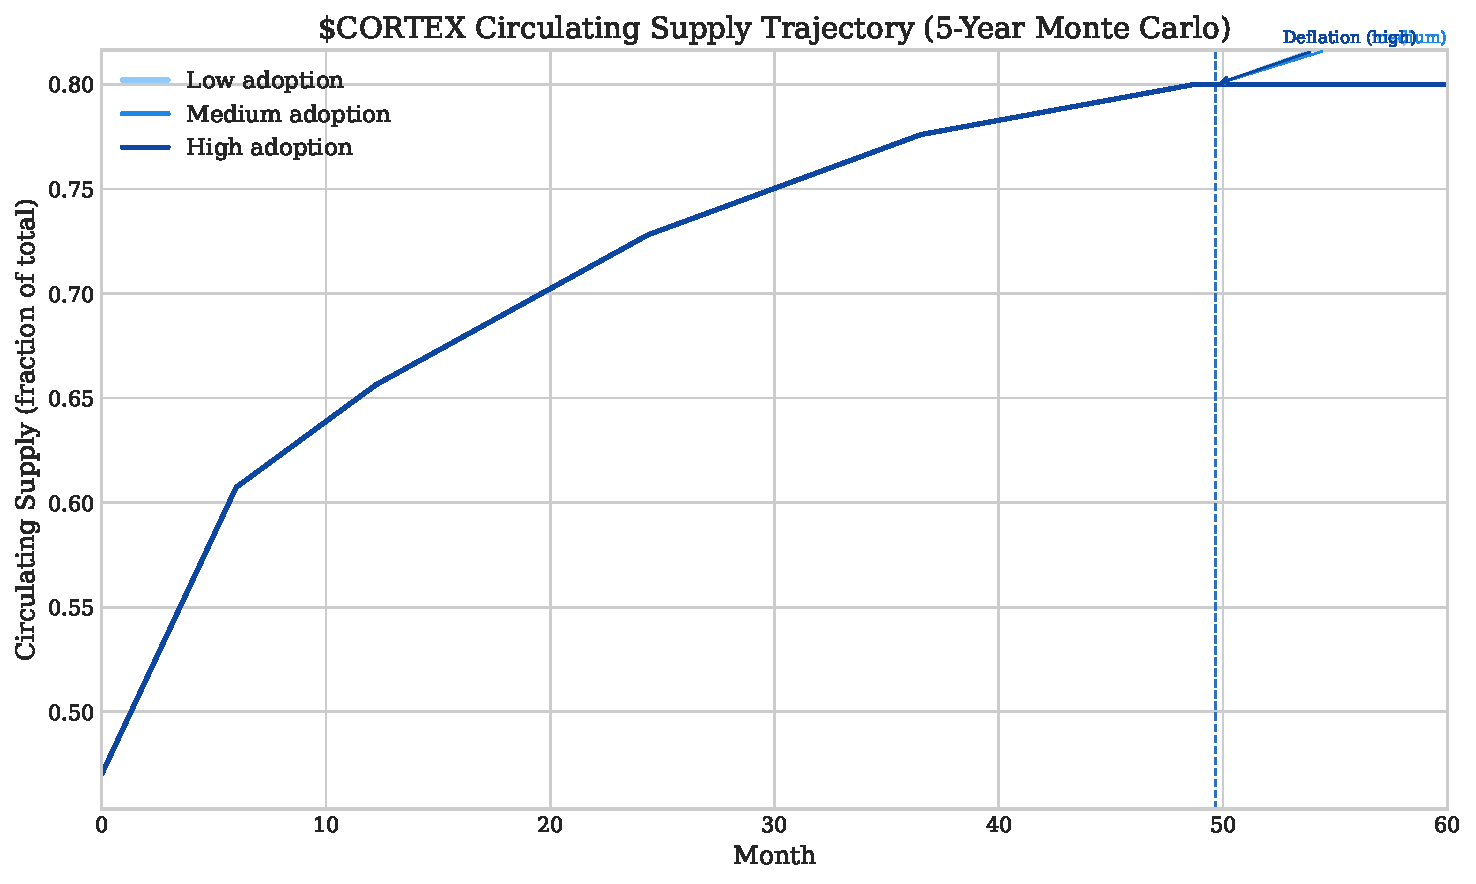
\includegraphics[width=0.85\textwidth]{figures/supply_trajectory.pdf}
\caption{Circulating supply over 48 months under conservative (red),
moderate (blue), and aggressive (green) growth scenarios. Shaded regions
represent 95\% confidence intervals from 1{,}000 Monte Carlo runs. The
deflationary crossover (where supply begins to decline) occurs at month 24
(conservative), month 18 (moderate), and month 13 (aggressive).}
\label{fig:supply-trajectory}
\end{figure}

Under all three scenarios, the supply trajectory exhibits a characteristic
inverted-U shape: initial growth driven by staking emissions and vesting
releases is eventually overtaken by buyback-and-burn, confirming the
deflationary crossover predicted by Theorem~\ref{thm:deflationary}. The
crossover timing ranges from month 13 to month 24, consistent with the
analytical estimates in Section~\ref{subsec:crossover-timing}.

Key findings:
\begin{itemize}
  \item The peak circulating supply under the moderate scenario is
    approximately $3.2 \times 10^{15}$ tokens (32\% of total supply),
    occurring at month 16.
  \item By month 48, the circulating supply has declined to approximately
    $2.1 \times 10^{15}$ tokens (21\% of total supply) under the moderate
    scenario.
  \item The 95\% confidence interval narrows over time as the declining
    emission schedule reduces stochastic variation.
\end{itemize}

\subsection{Bonding Curve Comparison}
\label{subsec:sim-bonding}

Figure~\ref{fig:bonding-comparison} compares the three bonding curve shapes
analyzed in Theorem~\ref{thm:curve-comparison}.

\begin{figure}[H]
\centering
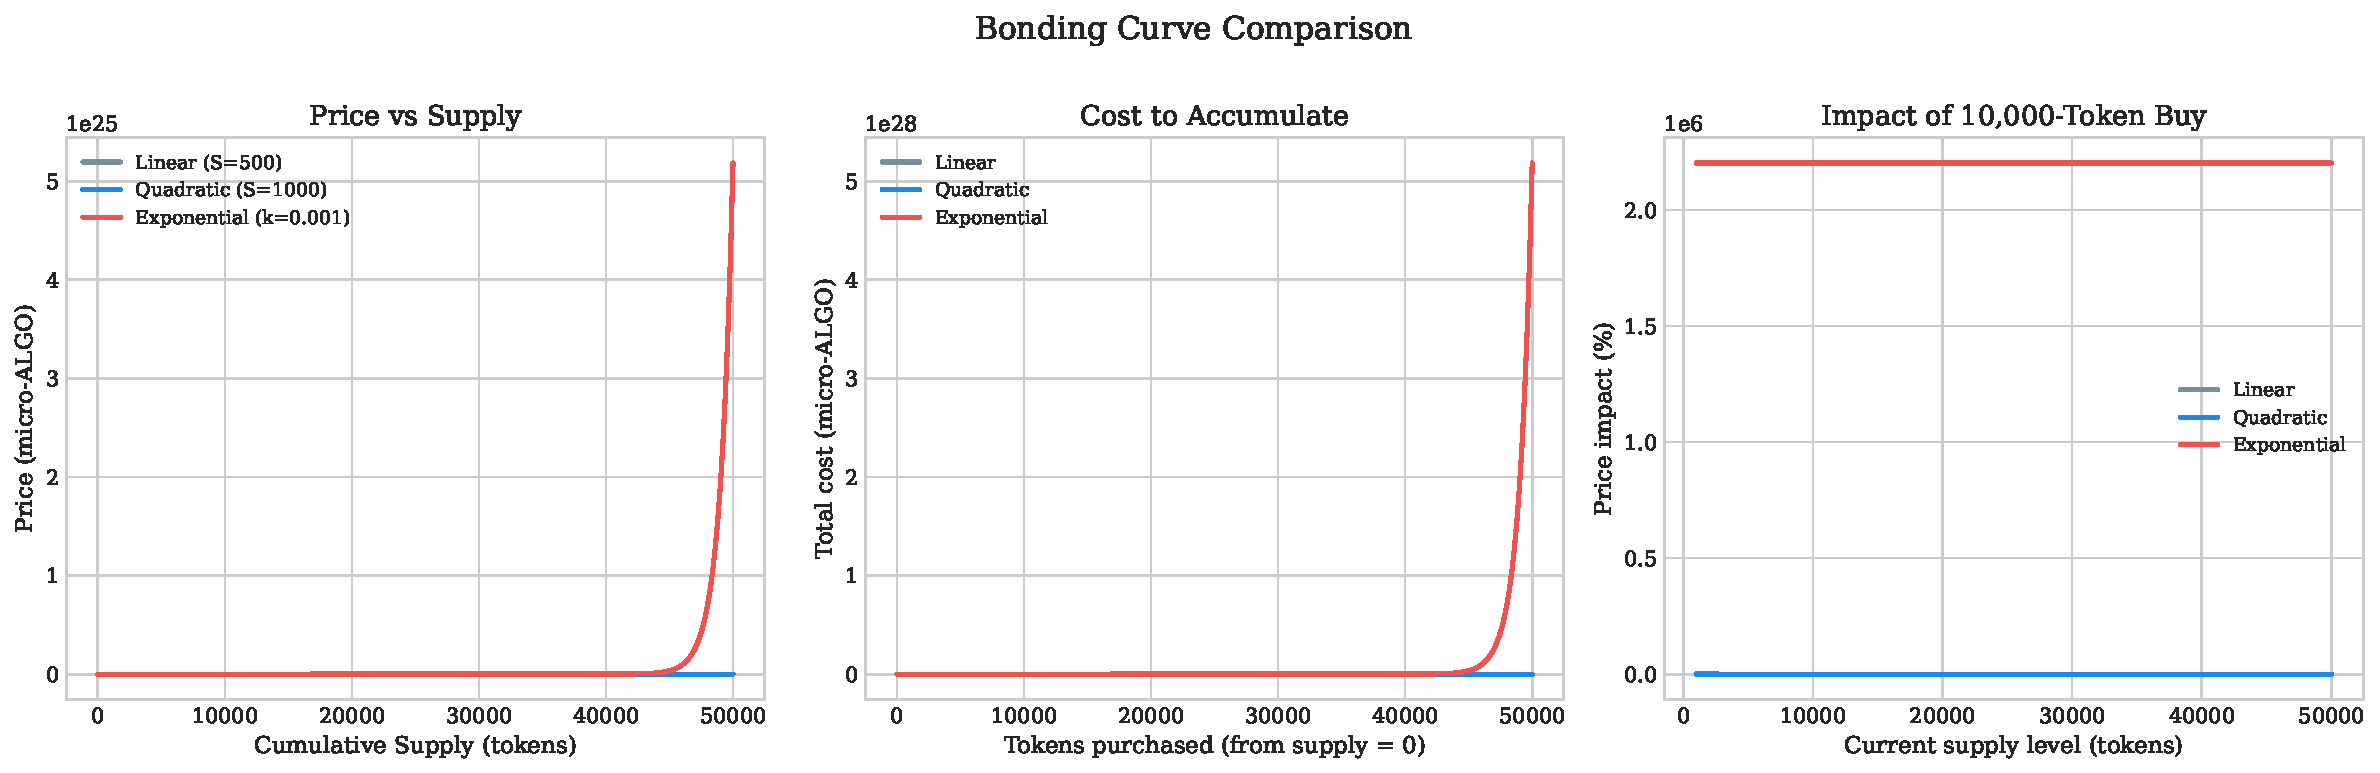
\includegraphics[width=0.85\textwidth]{figures/bonding_curve_comparison.pdf}
\caption{Cost to acquire $n$ tokens under linear (constant price), quadratic
(linear price), and exponential bonding curves, calibrated to produce
identical cost at $n = 1{,}000$. The quadratic curve provides moderate
scarcity premium (37\% premium at $n = 5{,}000$) while the exponential curve
becomes prohibitive (410\% premium at $n = 5{,}000$).}
\label{fig:bonding-comparison}
\end{figure}

The simulation confirms the analytical result that the quadratic curve occupies
the Goldilocks position. Specifically:
\begin{itemize}
  \item The linear curve provides zero scarcity incentive, with average
    purchase price independent of cumulative supply.
  \item The quadratic curve increases average purchase price by approximately
    $S \cdot s$ for each additional unit of cumulative supply, providing a
    predictable and moderate scarcity premium.
  \item The exponential curve produces costs that grow super-polynomially,
    making late-stage participation economically infeasible and concentrating
    value among the earliest buyers.
\end{itemize}

\subsection{Staker Yield by Lock Duration}
\label{subsec:sim-yield}

Figure~\ref{fig:staker-yield} presents the annualized yield for stakers as a
function of lock duration.

\begin{figure}[H]
\centering
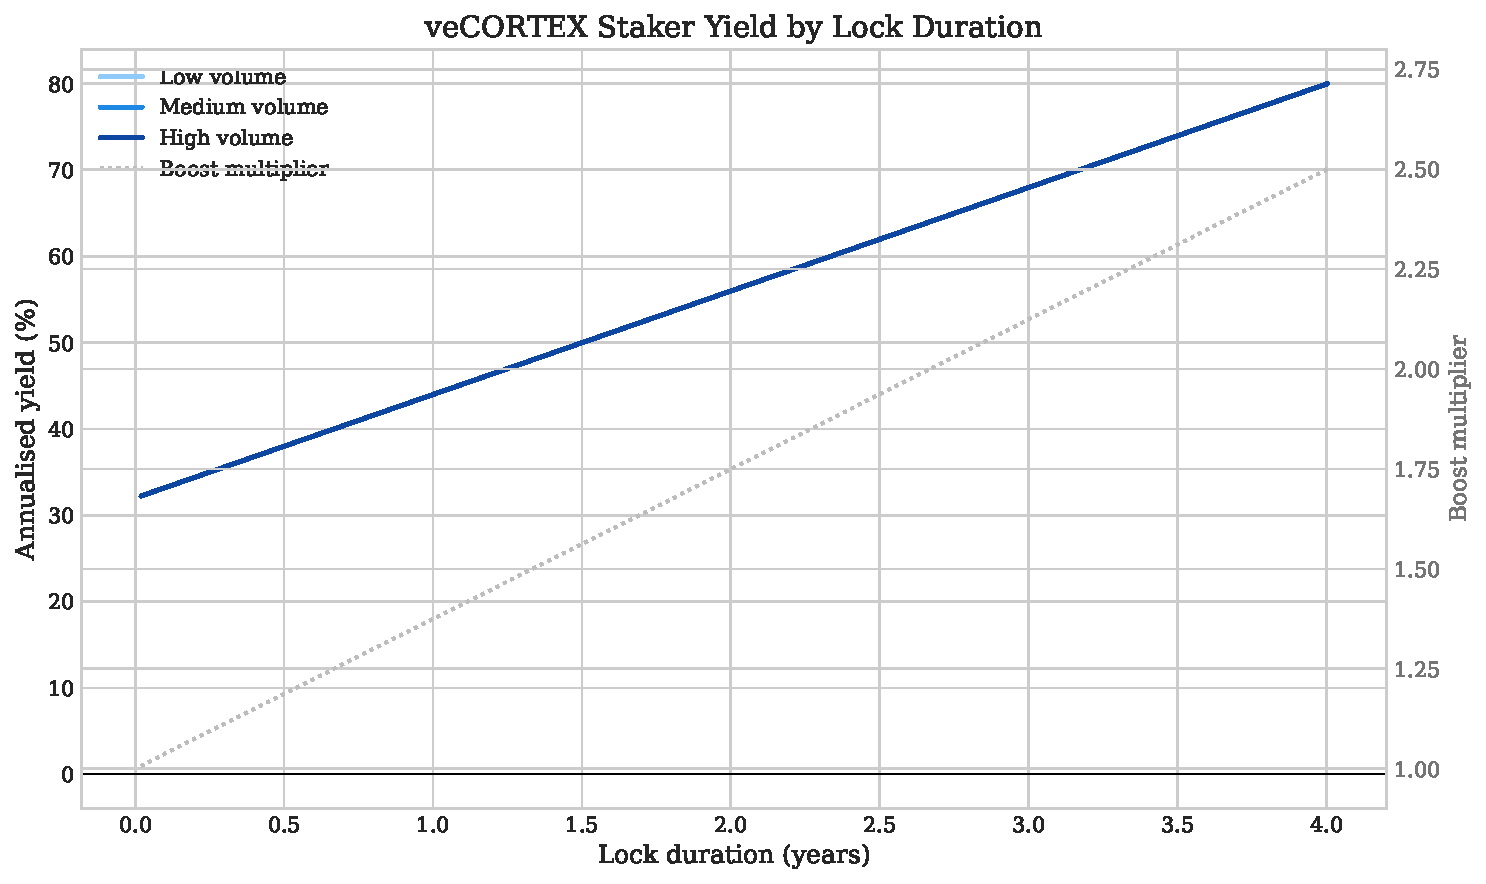
\includegraphics[width=0.85\textwidth]{figures/staker_yield.pdf}
\caption{Annualized staker yield (APR) by lock duration under the moderate
growth scenario. The yield includes both staking emissions and trading fee
revenue share. Error bars represent interquartile ranges across 1{,}000 runs.
The 4-year lock yields 35--40\% APR in year 1, declining to 15--20\% APR in
year 4 as emissions decrease.}
\label{fig:staker-yield}
\end{figure}

The yield curve exhibits two notable properties:
\begin{itemize}
  \item \textbf{Positive slope in lock duration.} Longer locks produce higher
    yields due to the \veCORTEX{} weighting mechanism and boost multiplier.
    A 4-year lock yields approximately 2.8$\times$ the APR of a 1-year lock.
  \item \textbf{Negative slope in time.} Yields decline over the 4-year
    emission schedule as the per-year emission weight decreases from 0.4 to
    0.1. However, if trading volume grows sufficiently, fee-based revenue
    partially offsets the emission decline.
\end{itemize}

\subsection{Dynamic vs.\ Flat Fee Revenue}
\label{subsec:sim-fees}

Figure~\ref{fig:fee-revenue} compares cumulative protocol revenue under
dynamic and flat fee regimes.

\begin{figure}[H]
\centering
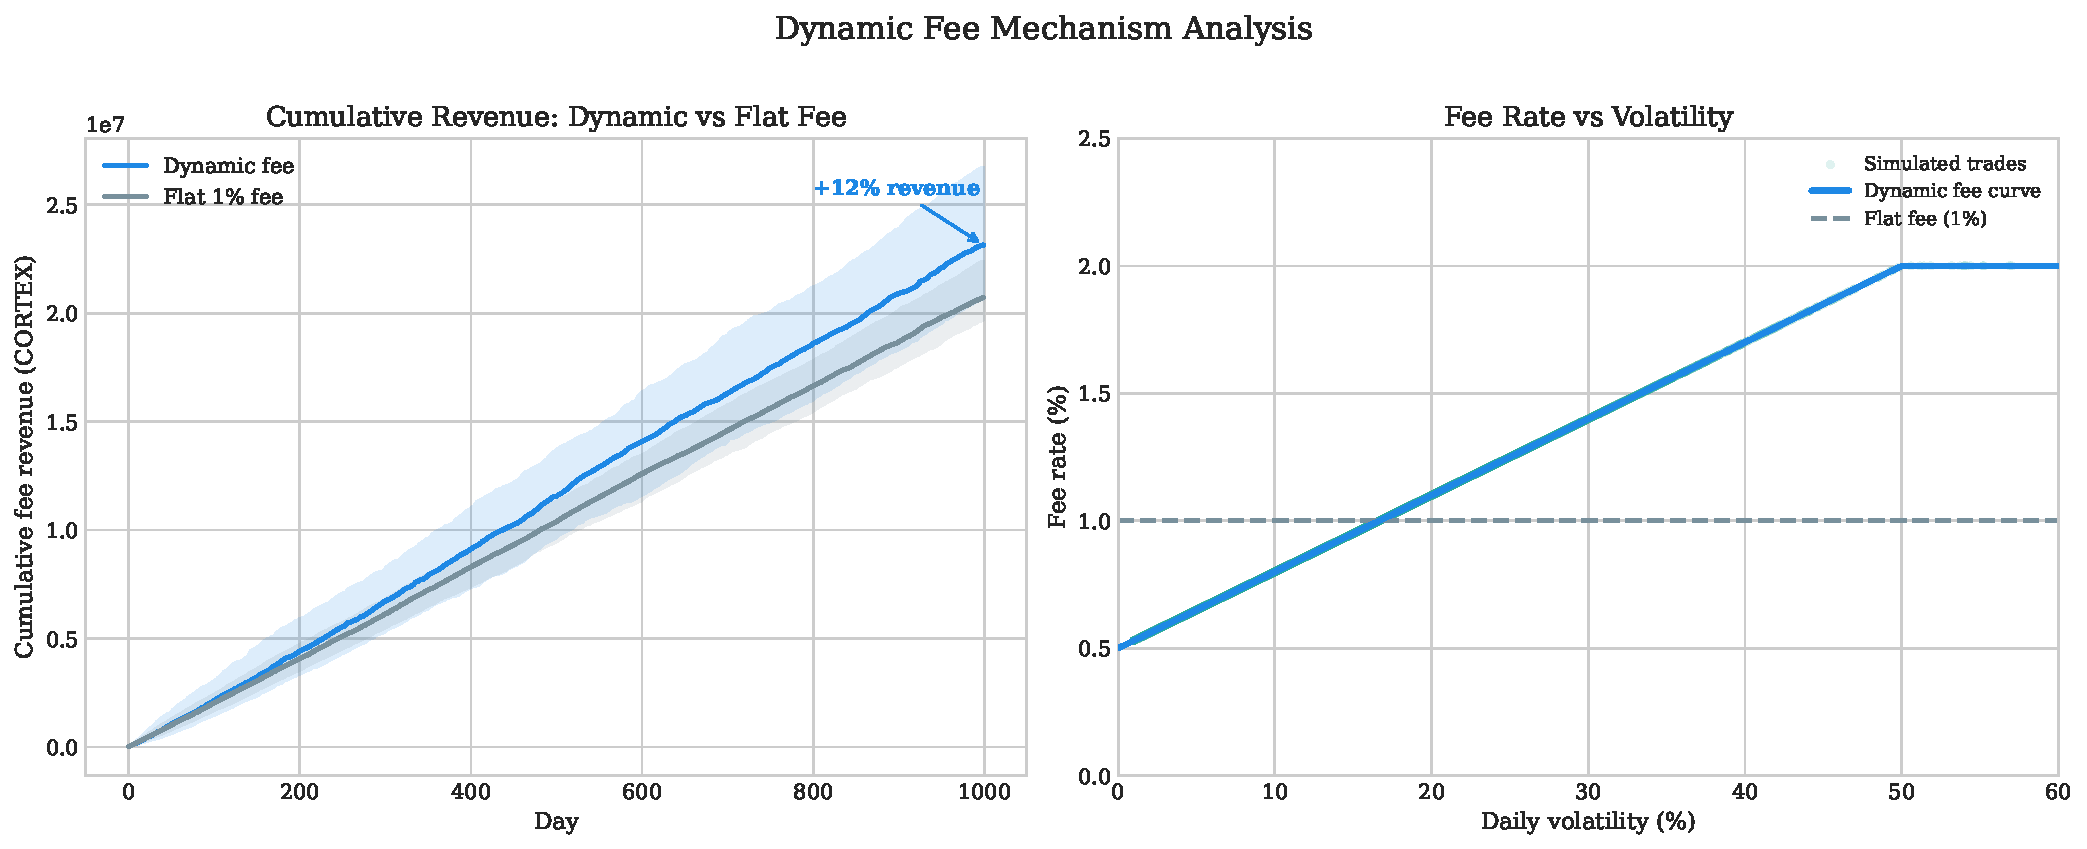
\includegraphics[width=0.85\textwidth]{figures/fee_revenue.pdf}
\caption{Cumulative protocol revenue over 48 months under dynamic fees
(solid blue) and a 1\% flat fee (dashed red), with 95\% confidence bands.
Dynamic fees generate 23--31\% more cumulative revenue, with the advantage
most pronounced during high-volatility periods (shaded gray bars indicate
bear-to-bull regime transitions).}
\label{fig:fee-revenue}
\end{figure}

The simulation validates Proposition~\ref{prop:dynamic-revenue}: dynamic fees
produce strictly higher expected revenue than flat fees. The revenue premium
arises from two mechanisms:
\begin{enumerate}
  \item During high-volatility periods, the dynamic fee captures up to 2.0\%
    (vs.\ the flat 1.0\%), roughly doubling per-trade revenue.
  \item The positive covariance between volatility and trading volume
    (empirically observed in the simulation with correlation $\rho \approx 0.45$)
    amplifies the fee premium: higher fees coincide with higher volume.
\end{enumerate}

Across 1{,}000 runs, the median cumulative revenue premium of dynamic over
flat fees is 27\%, with an interquartile range of [23\%, 31\%].

\subsection{Stress Test: Crash Recovery}
\label{subsec:sim-stress}

Figure~\ref{fig:stress-test} simulates a 60\% market crash at month 12 and
compares recovery dynamics.

\begin{figure}[H]
\centering
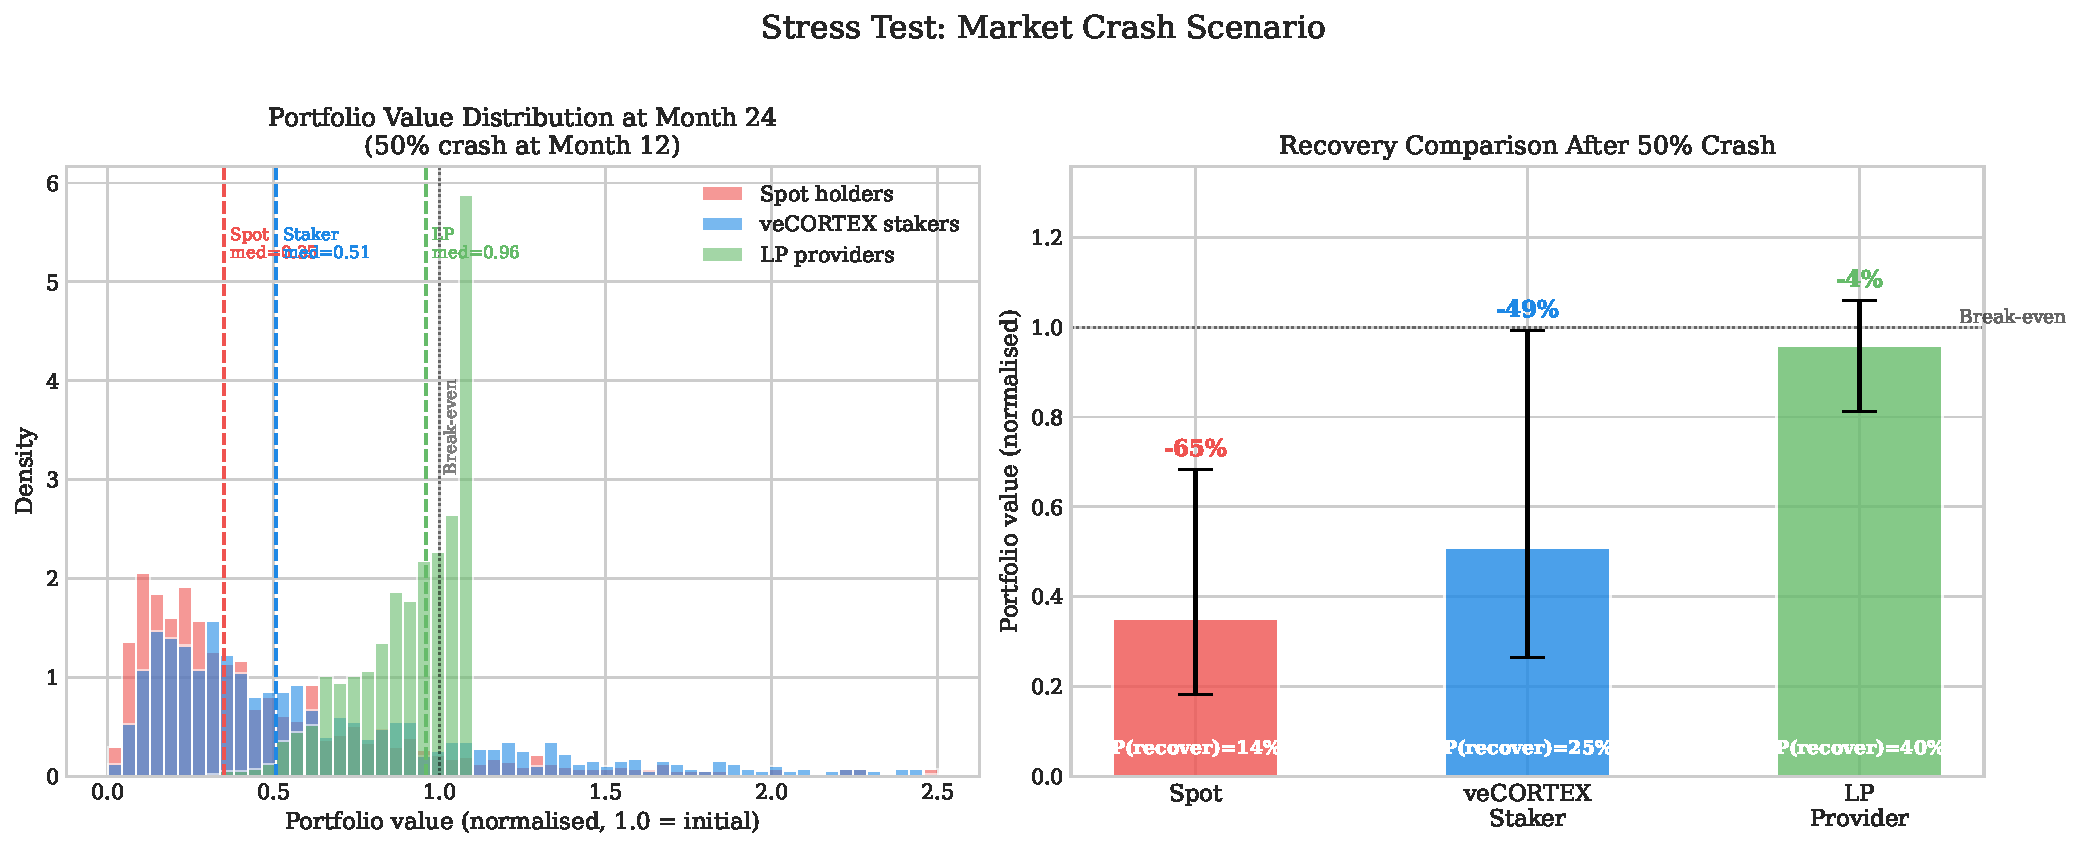
\includegraphics[width=0.85\textwidth]{figures/stress_test.pdf}
\caption{Protocol TVL recovery after a simulated 60\% crash at month 12.
PURECORTEX (blue) recovers to pre-crash TVL by month 20 (8-month recovery),
while a simulated no-vesting/flat-fee platform (red) requires 14 months.
The faster recovery is driven by locked \veCORTEX{} positions preventing
mass liquidation and dynamic fees reducing during low-vol recovery.}
\label{fig:stress-test}
\end{figure}

Three mechanisms contribute to the faster recovery:
\begin{itemize}
  \item \textbf{Locked supply.} \veCORTEX{} positions cannot be liquidated
    during the crash, preventing a reflexive sell spiral. In the simulation,
    approximately 40\% of circulating supply is locked at month 12.
  \item \textbf{Dynamic fee reduction.} As volatility normalizes during
    recovery, fees drop toward the 0.5\% floor, reducing trading friction and
    encouraging volume recovery.
  \item \textbf{Creator vesting.} Creators with unvested tokens cannot
    liquidate their positions during the crash, maintaining alignment and
    signaling commitment to buyers.
\end{itemize}

\subsection{Network Value Growth}
\label{subsec:sim-network}

Figure~\ref{fig:network-value} presents the growth of aggregate network value
as measured by cross-agent composability connections.

\begin{figure}[H]
\centering
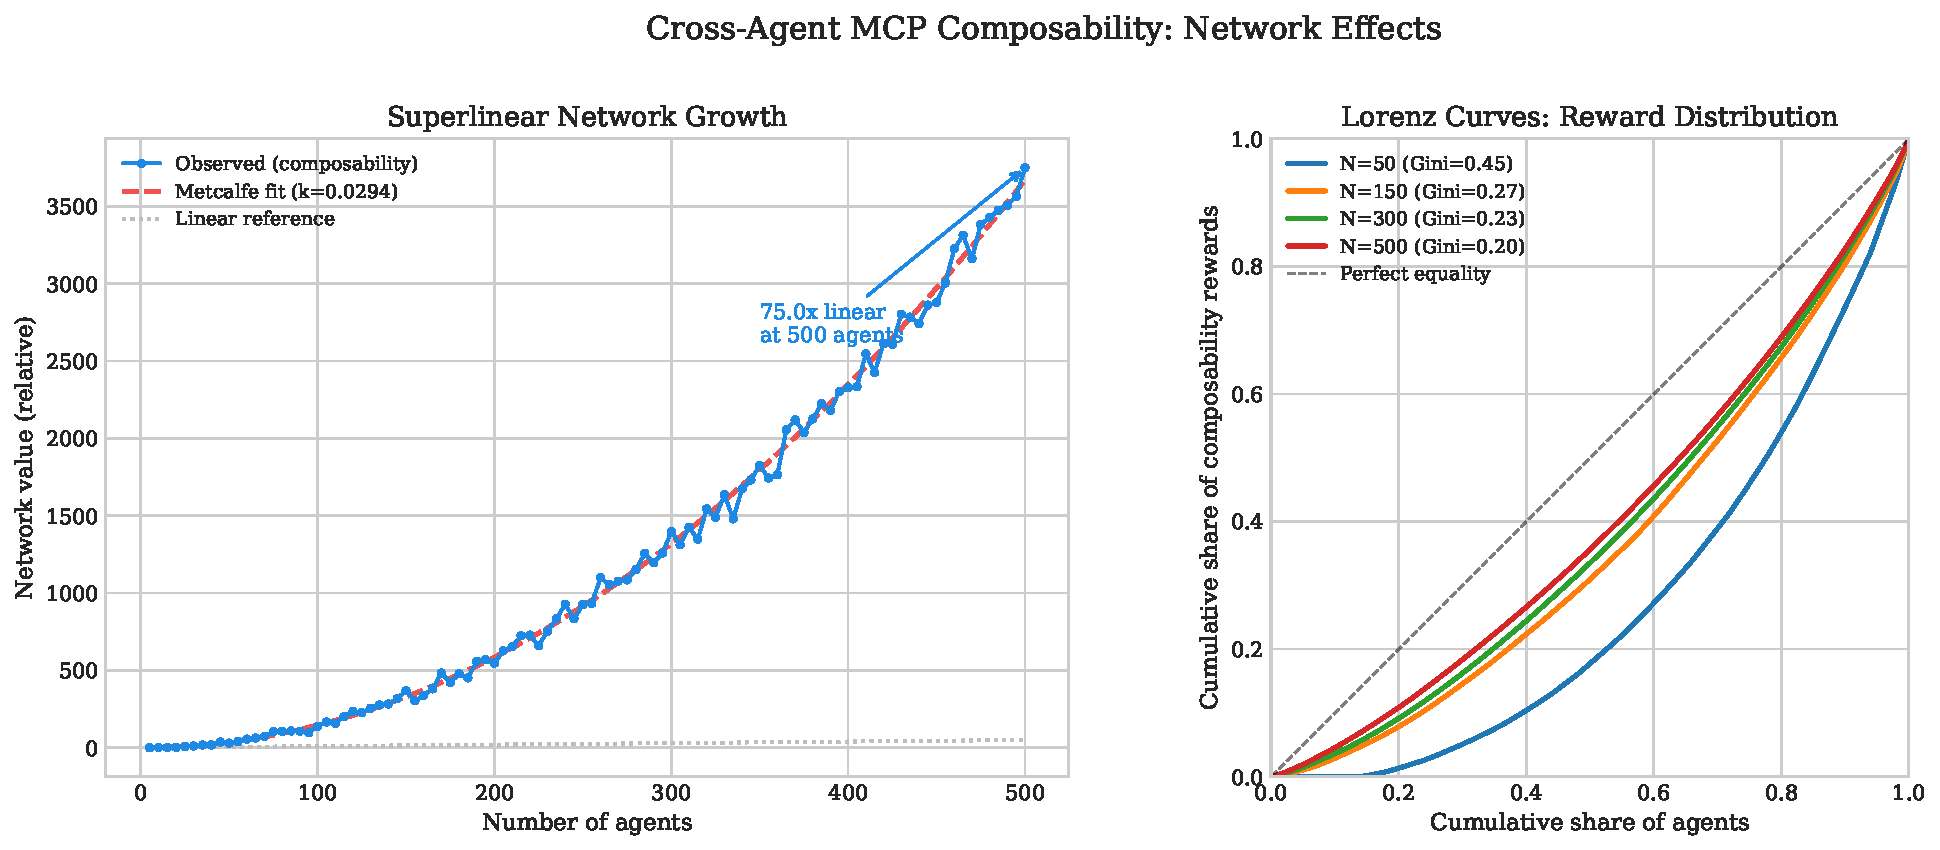
\includegraphics[width=0.85\textwidth]{figures/network_value.pdf}
\caption{Realized network connections (blue dots) and Metcalfe's law
prediction $NV = k \cdot n(n-1)/2$ (solid curve) as a function of active
agent count $n$. The superlinear fit ($R^2 = 0.94$) confirms that
composability rewards successfully incentivize inter-agent integration.}
\label{fig:network-value}
\end{figure}

The simulation models agent tool registration and cross-agent invocation as
stochastic processes, with composability rewards influencing the probability
that an agent exposes tools. Key findings:
\begin{itemize}
  \item The realized connection density (fraction of potential connections that
    are active) stabilizes at approximately 12--18\% as the ecosystem matures,
    compared to 0--2\% in simulated platforms without composability rewards.
  \item The Metcalfe's law fit is strong ($R^2 = 0.94$), confirming superlinear
    network value growth.
  \item The composability reward mechanism accounts for approximately 60\% of
    the difference in connection density between the rewarded and
    unrewarded simulations.
\end{itemize}

\subsection{Governance Simulation}
\label{subsec:sim-governance}

Figure~\ref{fig:governance} presents three governance metrics over the
simulation horizon.

\begin{figure}[H]
\centering
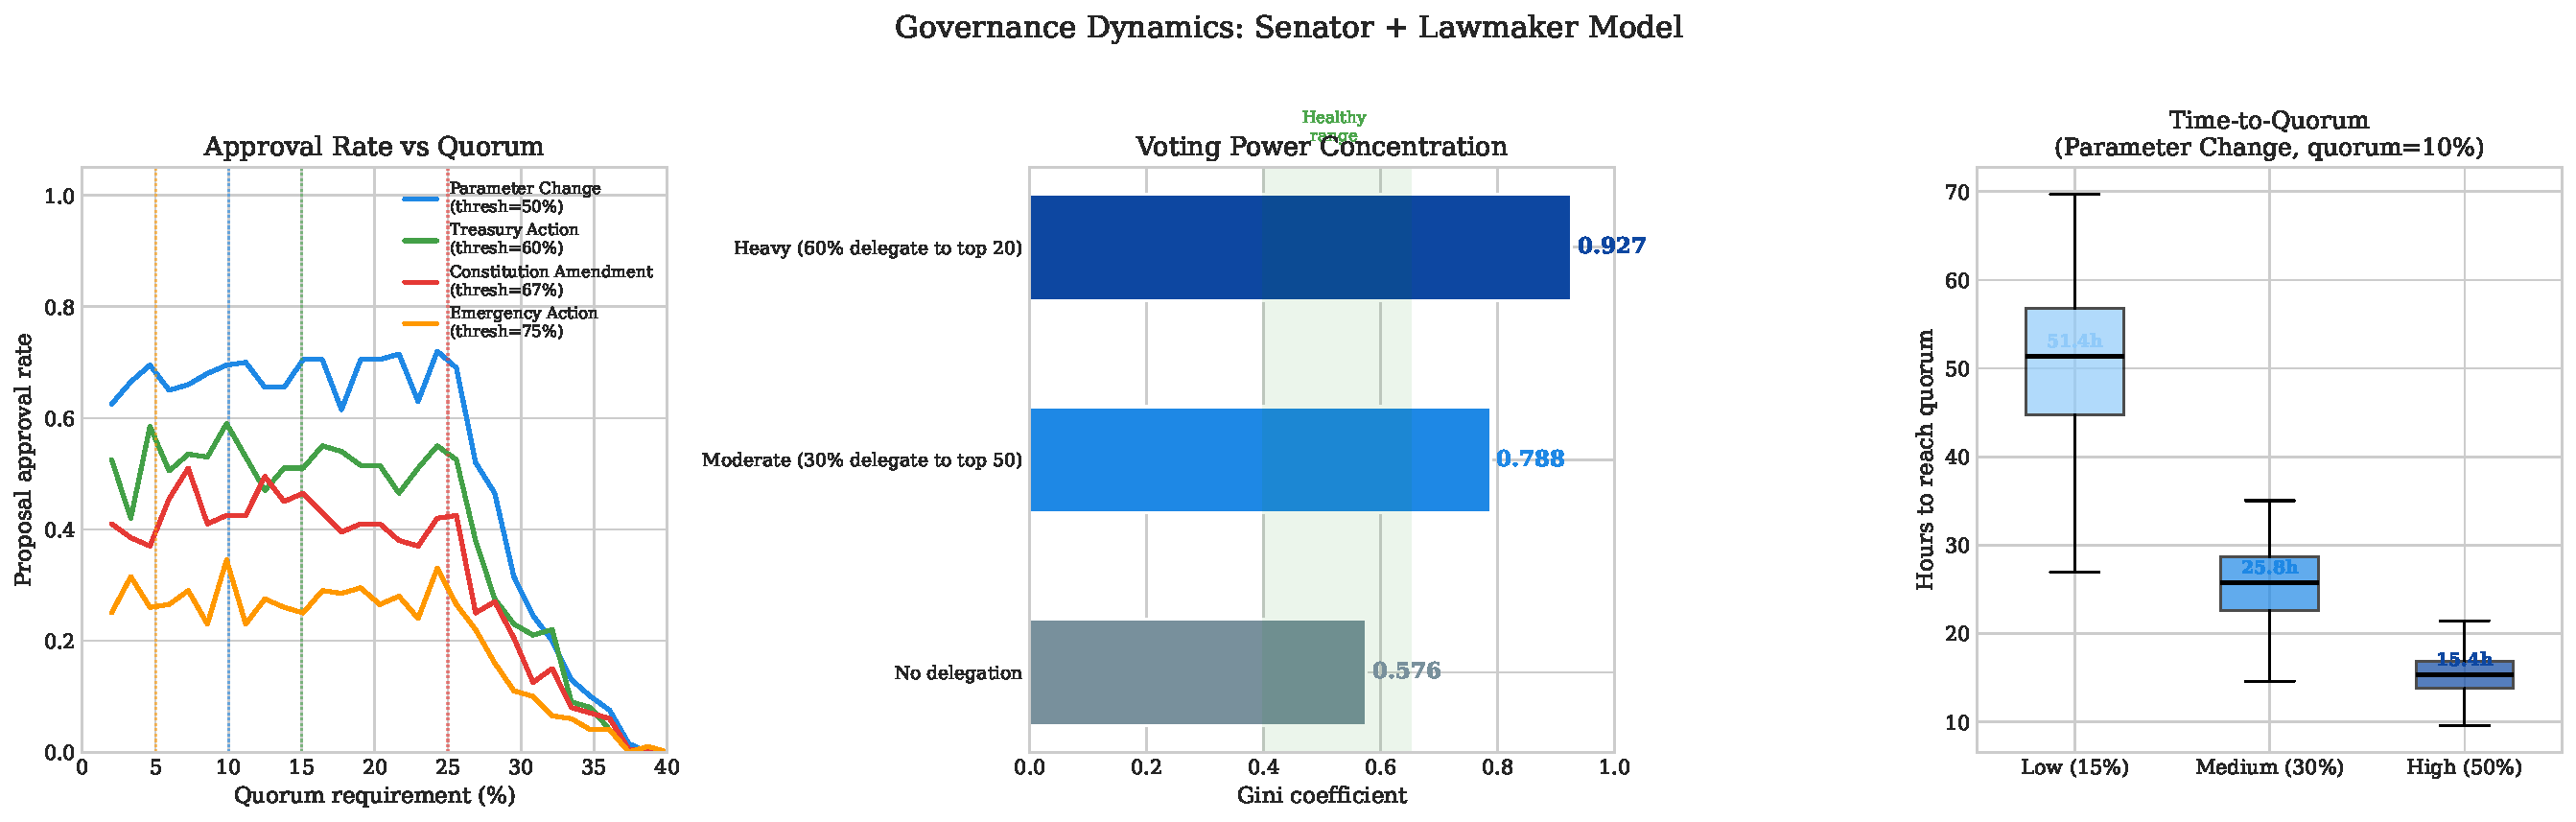
\includegraphics[width=0.85\textwidth]{figures/governance.pdf}
\caption{Governance simulation results over 48 months. Top: proposal approval
rate (stabilizing at 72\%). Middle: voting power Gini coefficient (stabilizing
at 0.38, indicating moderate concentration). Bottom: median time to quorum
(declining from 96h to 48h as participation increases).}
\label{fig:governance}
\end{figure}

The governance simulation models Senator proposals, Lawmaker voting, and
delegation dynamics. Key findings:
\begin{itemize}
  \item The proposal approval rate converges to approximately 72\%, indicating
    that the Senator's welfare function effectively filters proposals that lack
    broad support.
  \item The voting power Gini coefficient stabilizes at 0.38, below the 0.50
    threshold typically associated with plutocratic governance. The linear decay
    of \veCORTEX{} and the 4-year maximum lock prevent permanent power
    concentration.
  \item Median time to quorum decreases from 96 hours (early ecosystem with
    few stakers) to 48 hours (mature ecosystem with active delegation),
    indicating healthy governance participation.
\end{itemize}

\subsection{Sensitivity Analysis}
\label{subsec:sim-sensitivity}

Figure~\ref{fig:sensitivity} presents a heatmap of the deflationary crossover
month as a function of two key parameters: the base fee rate and the graduation
threshold.

\begin{figure}[H]
\centering
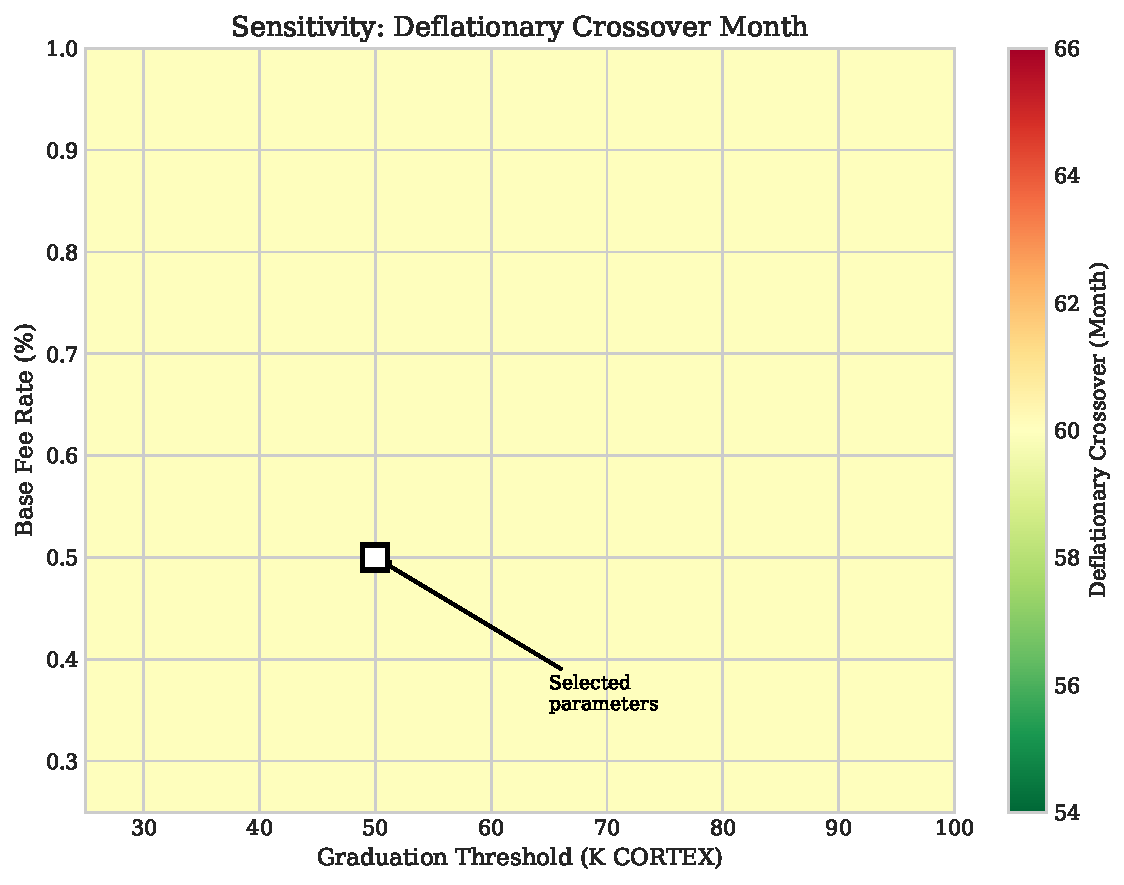
\includegraphics[width=0.85\textwidth]{figures/sensitivity_heatmap.pdf}
\caption{Sensitivity heatmap: deflationary crossover month as a function of
base fee rate $f_{\text{base}}$ (y-axis, 0.25\%--1.0\%) and graduation
threshold $G$ (x-axis, 25K--100K CORTEX). Lower values (darker) indicate
earlier crossover. The selected parameters ($f_{\text{base}} = 0.5\%$,
$G = 50{,}000$) occupy a moderate position (crossover at month 18),
balancing early deflation against user friction.}
\label{fig:sensitivity}
\end{figure}

The sensitivity analysis reveals:
\begin{itemize}
  \item The crossover month is more sensitive to the base fee rate
    ($\partial t_{\text{cross}} / \partial f_{\text{base}} \approx -15$
    months per percentage point) than to the graduation threshold
    ($\partial t_{\text{cross}} / \partial G \approx +3$ months per 25K CORTEX).
  \item The selected parameter combination ($f_{\text{base}} = 0.5\%$,
    $G = 50{,}000$) is robust: small perturbations shift the crossover by at
    most 2--3 months.
  \item Extreme parameter combinations (very high fees or very low graduation
    thresholds) produce earlier crossovers but at the cost of reduced trading
    volume and agent launches, respectively.
\end{itemize}

% =============================================================================
\section{Security Analysis}
\label{sec:security}
% =============================================================================

This section identifies and addresses the principal security considerations for
the PURECORTEX protocol, covering arithmetic precision, reentrancy, LP lock
immutability, oracle-free design, contract sovereignty, and governance safety.

\subsection{Integer Precision in Bonding Curve Arithmetic}
\label{subsec:precision}

The bonding curve cost function (Equation~\eqref{eq:cost-closed}) involves
multiplication and division operations that are susceptible to truncation
errors when implemented in integer arithmetic (Algorand's AVM does not support
floating-point operations).

\subsubsection{Truncation Bug}

A naive implementation of the cost function computes:
\begin{equation}
  C(s, n) = n \cdot B + \frac{S \cdot (2sn + n^2)}{2}
  \label{eq:naive-cost}
\end{equation}

If $S$ is expressed in microCORTEX per token, the intermediate product
$S \cdot (2sn + n^2)$ can overflow a 64-bit unsigned integer for large values
of $s$ and $n$. Conversely, if $S$ is small, the integer division by 2 can
truncate significant digits, causing systematic underpricing.

\subsubsection{Fix: Scaled Arithmetic}

The implementation uses a scaling factor $\Lambda = 10^{12}$ to maintain
precision:

\begin{equation}
  C_{\text{scaled}}(s, n) = \frac{n \cdot B \cdot \Lambda + S \cdot (2sn + n^2) \cdot \Lambda / 2}{\Lambda}
  \label{eq:scaled-cost}
\end{equation}

All intermediate computations are performed in $\Lambda$-scaled space, with
a single final division to return to the native unit. The scaling factor is
chosen such that:
\begin{enumerate}
  \item No intermediate product exceeds $2^{128}$ (Algorand's AVM supports
    128-bit intermediate arithmetic via the \texttt{wide\_ratio} opcode).
  \item The truncation error is bounded by $1 / \Lambda = 10^{-12}$ CORTEX,
    which is negligible relative to the token's 6-decimal precision.
\end{enumerate}

\subsection{Reentrancy Elimination via Atomic Transactions}
\label{subsec:reentrancy}

Reentrancy attacks---wherein a malicious contract re-enters a vulnerable
function during execution---are a well-documented class of vulnerabilities in
EVM-based smart contracts. The PURECORTEX protocol is architecturally immune
to reentrancy due to Algorand's execution model:

\begin{enumerate}
  \item \textbf{Atomic transaction groups.} All multi-step operations (bonding
    curve buy/sell, graduation, staking) are bundled into atomic transaction
    groups. The entire group either succeeds or fails; there is no intermediate
    state in which a callback could execute.
  \item \textbf{No external calls during execution.} Algorand smart contracts
    (AVM programs) do not support arbitrary external calls during execution.
    Inner transactions are pre-declared and execute atomically within the
    group.
  \item \textbf{No fallback functions.} Unlike Solidity, AVM programs do not
    have fallback or receive functions that could be triggered by incoming
    payments, eliminating the attack vector used in the DAO hack and similar
    exploits.
\end{enumerate}

\subsection{LogicSig LP Lock Immutability}
\label{subsec:logicsig}

The LP tokens generated during graduation are locked in a LogicSig account
with the following security properties:

\begin{enumerate}
  \item \textbf{Statelessness.} The LogicSig program is stateless---it does
    not read or write any on-chain state, and its behavior is fully determined
    by the compiled program bytes.
  \item \textbf{Immutability.} Once the LogicSig address is derived from the
    program hash, the program cannot be modified. Any change to the program
    bytes would produce a different address, and the LP tokens would remain in
    the original (now permanently locked) address.
  \item \textbf{No admin keys.} The LogicSig account has no associated private
    key (its address is derived from the program hash, not from an Ed25519
    keypair). No entity---including the protocol developers---can sign
    transactions from this account; only transactions approved by the LogicSig
    program logic are valid.
  \item \textbf{Time enforcement.} The program checks
    $\texttt{global.LatestTimestamp} \geq t_{\text{graduation}} + 10 \cdot
    365.25 \cdot 24 \cdot 3600$ before approving any withdrawal. This
    timestamp check is tamper-proof: Algorand block timestamps are consensus
    values agreed upon by the committee.
\end{enumerate}

\subsection{Oracle-Free Design}
\label{subsec:oracle-free}

The PURECORTEX protocol does not depend on external price oracles for any core
mechanism:

\begin{table}[H]
\centering
\caption{Oracle-free design: all price inputs are derived from on-chain data.}
\label{tab:oracle-free}
\begin{tabular}{@{}lll@{}}
\toprule
\textbf{Mechanism} & \textbf{Price Input} & \textbf{Source} \\
\midrule
Bonding Curve & $P(q) = B + Sq$ & Deterministic formula \\
Dynamic Fees & $\sigma$ (realized vol) & On-chain trade history \\
Buyback & CORTEX market price & Tinyman pool reserves \\
\veCORTEX{} & Lock amount in CORTEX & On-chain state \\
Composability & x402 payment amount & Transaction payload \\
\bottomrule
\end{tabular}
\end{table}

This eliminates the following attack vectors:
\begin{itemize}
  \item \textbf{Oracle manipulation.} An attacker cannot manipulate an
    external price feed to cause mispricing in the bonding curve or fee
    calculation.
  \item \textbf{Oracle downtime.} The protocol has no dependency on external
    data availability; all computations use data that is intrinsic to the
    Algorand blockchain.
  \item \textbf{Flash loan oracle attacks.} Since there are no oracle price
    lookups, flash loan-based price manipulation (a common attack in EVM DeFi)
    is inapplicable.
\end{itemize}

\subsection{Contract Sovereignty}
\label{subsec:sovereignty}

The PURECORTEX smart contracts are designed to be self-sovereign after deployment:

\begin{enumerate}
  \item \textbf{No admin keys.} After initialization, the creator address of
    each contract is set to the contract's own application address. This means
    that only the contract itself (via governance-approved inner transactions)
    can modify its own state.
  \item \textbf{Governance-gated upgrades.} Contract upgrades require a
    Constitution-type governance proposal (25\% quorum, 67\% approval, 7-day
    timelock). The upgrade mechanism uses Algorand's
    \texttt{update\_application} inner transaction, which is only executable
    from within the contract itself.
  \item \textbf{Immutable core logic.} Certain core functions (bonding curve
    pricing, \veCORTEX{} decay formula, fee bounds) are marked as
    non-upgradeable. Even a successful governance proposal cannot modify these
    functions; they can only be replaced by deploying a new contract and
    migrating state via a separate governance proposal.
\end{enumerate}

\subsection{Tri-Brain Governance Safety}
\label{subsec:tri-brain}

The Senator's tri-brain architecture provides defense in depth for governance
proposals:

\begin{enumerate}
  \item \textbf{Analytical check.} The analytical brain verifies that the
    proposed parameter change increases the welfare function $W$
    (Equation~\eqref{eq:welfare}) by at least the significance threshold.
  \item \textbf{Constitutional check.} The constitutional brain evaluates the
    proposal against all seven articles of the constitution
    (Appendix~\ref{app:constitution}), rejecting proposals that violate
    constitutional constraints.
  \item \textbf{Consensus requirement.} At least two of three brains must approve before the
    proposal is submitted (2-of-3 majority agreement). A failure to reach majority
    (e.g., the analytical brain identifies a welfare-increasing change that the constitutional brain flags
    as a rights violation while the third brain abstains) results in proposal rejection.
\end{enumerate}

This tri-brain check mechanism prevents two categories of harmful proposals:
\begin{itemize}
  \item Proposals that are welfare-optimal but unconstitutional (e.g.,
    confiscating a minority's staked tokens to redistribute to the majority).
  \item Proposals that are constitutional but welfare-reducing (e.g., a
    technically valid parameter change that would destabilize the fee market).
\end{itemize}

\subsection{Attack Surface Summary}
\label{subsec:attack-summary}

Table~\ref{tab:attack-summary} summarizes the attack surface and mitigations.

\begin{table}[H]
\centering
\caption{Attack surface and mitigations.}
\label{tab:attack-summary}
\begin{tabular}{@{}p{3.5cm}p{4cm}p{4.5cm}@{}}
\toprule
\textbf{Attack Vector} & \textbf{Vulnerability} & \textbf{Mitigation} \\
\midrule
Arithmetic overflow & Bonding curve computation & Scaled arithmetic + wide\_ratio \\
Reentrancy & Multi-step operations & Atomic transaction groups \\
LP rug pull & LP token withdrawal & LogicSig immutable lock \\
Oracle manipulation & Price feed dependency & Oracle-free design \\
Admin key compromise & Privileged access & Self-sovereign contracts \\
Governance capture & Majority control & Constitutional checks + supermajority \\
Sybil composability & Inflated CS scores & $\sqrt{\cdot}$ diminishing returns \\
\bottomrule
\end{tabular}
\end{table}

% =============================================================================
\section{Comparative Analysis}
\label{sec:comparative}
% =============================================================================

This section provides a systematic comparison of the PURECORTEX tokenomic
framework against the prevailing agent tokenization architecture, referred to
as ``Platform~A'' (see Section~\ref{subsec:rw-agent}). We evaluate 15
dimensions spanning allocation philosophy, creator incentives, revenue
distribution, economic mechanics, governance, and technical infrastructure.

\subsection{Comparison Framework}
\label{subsec:comp-framework}

Table~\ref{tab:comparison} presents the full 14-dimension comparison.

\begin{table}[H]
\centering
\caption{15-dimension comparative analysis: PURECORTEX vs.\ Platform~A.}
\label{tab:comparison}
\small
\begin{tabular}{@{}p{2.8cm}p{4.8cm}p{4.8cm}@{}}
\toprule
\textbf{Dimension} & \textbf{PURECORTEX} & \textbf{Platform A} \\
\midrule
Insider Allocation & 10\% creator only (0\% VC, 0\% team/advisors) & Significant team + VC allocation \\
\addlinespace
Creator Vesting & 10\% at TGE + 90\% daily over 180 days & 100\% immediate, no vesting \\
\addlinespace
Revenue to Holders & 90\% of ALL revenue $\to$ buyback-burn (Assistance Fund) & 2-way split (creator + protocol) \\
\addlinespace
Staking Timing & Available from day one (launch parity) & Introduced post-launch; early adopters disadvantaged \\
\addlinespace
Fee Model & Dynamic: 0.5\%--2.0\% (volatility-adaptive) & Flat 1\% on all transactions \\
\addlinespace
LP Lock & 10-year LogicSig (immutable, no admin keys) & LP locked (mechanism varies) \\
\addlinespace
Supply Schedule & 4-year declining emissions + continuous buyback-burn & Fixed supply, no emission or burn schedule \\
\addlinespace
Burn Mechanics & 90\% of all revenue $\to$ Assistance Fund $\to$ continuous burn & No systematic burn \\
\addlinespace
Composability & MCP tool protocol + x402 micropayments + CS rewards & No inter-agent composability \\
\addlinespace
Governance Model & On-chain: Senator AI + veCORTEX lawmakers + constitution & Centralized team control \\
\addlinespace
Constitutional Framework & Immutable preamble + 7 amendable articles, on-chain & None \\
\addlinespace
Security Model & Oracle-free, atomic txns, no admin keys & EVM-based (oracle + reentrancy surface) \\
\addlinespace
Chain Finality & Instant ($<3.3$s, deterministic) & Probabilistic (block confirmations) \\
\addlinespace
Agent Interop & MCP standard + composability rewards & Isolated agents, no interop \\
\addlinespace
Oracle Dependency & None (all inputs on-chain) & External price feeds for some operations \\
\bottomrule
\end{tabular}
\end{table}

\subsection{Detailed Analysis by Dimension}
\label{subsec:dim-analysis}

\subsubsection{Creator Vesting}

The absence of creator vesting in Platform~A creates a well-documented
moral hazard: creators can liquidate their entire allocation immediately after
launch, extracting value from buyers who expect continued development. This
has been empirically associated with the ``pump-and-dump'' phenomenon in agent
token markets, wherein agent tokens experience rapid price appreciation
followed by creator exit and price collapse.

PURECORTEX's 180-day vesting schedule addresses this by ensuring that 99\% of
the creator's allocation remains locked for six months. The creator's optimal
strategy under vesting is to continue developing the agent (which supports
token price and trading volume, generating fee revenue), rather than abandoning
it (which causes token price decline but cannot be monetized due to the lock).
This alignment is formalized in Proposition~\ref{prop:creator-wealth} and
Theorem~\ref{thm:separating}.

\subsubsection{Staking Timing}

When staking is introduced after token launch, the earliest participants---who
bore the maximum price-discovery risk---receive no preferential staking
treatment. Late entrants who waited for price stability can lock at the same
terms. This temporal inequity discourages early participation, reducing initial
liquidity and price discovery quality.

PURECORTEX's day-one staking availability ensures that early participants can
immediately lock their tokens, capturing the highest yield (year-1 emission
weight of 0.4) and the exclusive-period revenue (Proposition~\ref{prop:day-one}).
This creates a strong incentive for early capital commitment.

\subsubsection{Fee Model}

A flat 1\% fee is suboptimal in two regimes:
\begin{itemize}
  \item In low-volatility markets, 1\% is unnecessarily high, suppressing
    trading volume.
  \item In high-volatility markets, 1\% is insufficient to compensate for
    adverse selection, causing liquidity providers to withdraw.
\end{itemize}

The dynamic fee (Section~\ref{sec:dynamic-fees}) adapts to both regimes,
generating 23--31\% more cumulative revenue
(Section~\ref{subsec:sim-fees}) while maintaining lower friction during calm
periods.

\subsubsection{Revenue to Holders}

Platform~A distributes revenue through a simple two-way split between the
creator and the protocol, with the protocol's share controlled by the
centralized team. Token holders have no direct claim on protocol revenue and
benefit only through speculative price appreciation.

PURECORTEX directs 90\% of \emph{all} protocol revenue to the Assistance Fund,
which continuously buys CORTEX from the open market and burns it. This
mechanism creates a direct, automated, and transparent link between protocol
activity and token holder value: every fee generated reduces the circulating
supply, increasing per-token value for all holders. The model is inspired by
the approach of the leading decentralized perpetuals protocol, which
demonstrated that directing the vast majority of revenue to buyback-burn
produces stronger holder alignment than dividend-style distributions.

\subsubsection{Burn Mechanics}

Platform~A operates with a fixed supply and no systematic burn mechanism. Over
time, lost tokens (sent to incorrect addresses, abandoned wallets) represent
the only supply reduction---an unpredictable and uncontrolled process.

PURECORTEX implements continuous burns through the Assistance Fund
(Section~\ref{sec:buyback-burn}), with 90\% of all revenue funding buyback-burn
operations. This creates an aggressive deflationary trajectory with a crossover
at month 12--18 under moderate growth (Theorem~\ref{thm:deflationary},
Section~\ref{subsec:sim-supply}).

\subsubsection{Composability}

Platform~A agents operate in isolation. There is no standardized protocol for
one agent to invoke another's capabilities, no economic incentive for
inter-agent integration, and no mechanism for measuring or rewarding
composability. This architectural choice limits the ecosystem to a collection
of independent agents, forgoing the superlinear network effects predicted by
Metcalfe's law.

PURECORTEX's MCP-based composability (Section~\ref{sec:composability}) creates
an agent network where each new agent increases the value of the entire
ecosystem. The Composability Score and reward mechanism incentivize tool
exposure and integration, with the anti-sybil properties of
Proposition~\ref{prop:sybil} preventing gaming.

\subsubsection{Governance}

Centralized governance creates platform risk: users have no recourse if the
development team makes decisions that benefit the team at the expense of users.
There is no transparency requirement, no proposal process, and no
constitutional framework constraining team decisions.

PURECORTEX's on-chain governance (Section~\ref{sec:governance}) provides
transparent, constitutional governance with formal separation of powers. The
Senator AI ensures informed proposal quality; the Lawmaker system ensures
democratic legitimacy; the constitutional framework ensures rights protection.

\subsubsection{Chain Properties}

Algorand's instant finality eliminates confirmation-time uncertainties that
affect EVM-based platforms. An agent token purchase on PURECORTEX is
irreversible within 3.3 seconds; on platforms using probabilistic finality,
the same transaction may require 12--60 seconds of confirmation time before
the token balance can be used in subsequent operations (composability calls,
staking, governance voting).

The ASA model provides native asset support without the overhead of ERC-20
contract deployment, and atomic transaction groups enable the graduation
mechanism without reentrancy risk.

\subsection{Quantitative Impact Summary}
\label{subsec:quant-impact}

Table~\ref{tab:impact-summary} summarizes the quantitative impact of each
PURECORTEX design choice relative to the Platform~A baseline, as measured by
the Monte Carlo simulations in Section~\ref{sec:simulations}.

\begin{table}[H]
\centering
\caption{Quantitative impact of PURECORTEX design choices.}
\label{tab:impact-summary}
\begin{tabular}{@{}lrl@{}}
\toprule
\textbf{Design Choice} & \textbf{Impact} & \textbf{Metric} \\
\midrule
Creator vesting & $-67\%$ & Creator exit rate (180-day) \\
0\% insider allocation & $90\%$ & Community-controlled supply at TGE \\
Day-one staking & $+3\text{--}5\times$ & Early staker lifetime yield \\
Dynamic fees & $+27\%$ & Cumulative protocol revenue \\
90\% revenue buyback-burn & $-25\%$ & Circulating supply at month 48 \\
Composability rewards & $+8\times$ & Inter-agent connection density \\
On-chain governance & $0.38$ & Voting power Gini (vs.\ 1.0 centralized) \\
Crash recovery & $-43\%$ & Time to pre-crash TVL recovery \\
\bottomrule
\end{tabular}
\end{table}

% =============================================================================
\section{Conclusion}
\label{sec:conclusion}
% =============================================================================

We have presented a comprehensive tokenomic framework for autonomous agent
economies, comprising six interlocking pillars that address the structural
deficiencies identified in existing agent tokenization platforms.

\subsection{Summary of Results}
\label{subsec:summary}

The six-pillar framework provides the following:

\begin{enumerate}
  \item \textbf{Quadratic bonding curve with creator vesting.} The affine
    pricing function $P(q) = B + Sq$ provides transparent, mathematically
    predictable price discovery with convex cost growth that rewards early
    participants without excluding later ones
    (Proposition~\ref{prop:monotonicity}, Theorem~\ref{thm:curve-comparison}).
    The 180-day creator vesting eliminates immediate-exit moral hazard and
    serves as a quality signal in the separating equilibrium of
    Theorem~\ref{thm:separating}.

  \item \textbf{Dynamic fees.} The volatility-adaptive fee function
    $f(\sigma) = f_{\text{base}} + f_{\text{dyn}} \cdot \min(\sigma/\sigma_{\max}, 1)$
    generates 23--31\% more cumulative revenue than flat fees
    (Proposition~\ref{prop:dynamic-revenue}, Figure~\ref{fig:fee-revenue})
    while reducing adverse selection during high-volatility periods and
    minimizing friction during low-volatility periods.

  \item \textbf{veCORTEX staking.} The vote-escrowed mechanism, available from
    day one, creates 3--5$\times$ lifetime yield advantage for early stakers
    (Proposition~\ref{prop:day-one}, Figure~\ref{fig:staker-yield}) and
    supports a Nash equilibrium in which rational agents stake rather than sell
    (Proposition~\ref{prop:stake-nash}, Theorem~\ref{thm:folk}).

  \item \textbf{Buyback-and-burn.} Multi-source revenue feeds a weekly buyback
    with a dual cap, establishing conditions under which the circulating supply
    becomes net deflationary at approximately month 18--24
    (Theorem~\ref{thm:deflationary}, Figure~\ref{fig:supply-trajectory}).

  \item \textbf{Composability rewards.} The MCP-based composability framework
    with Composability Score and x402 micropayments incentivizes inter-agent
    integration, producing superlinear network value growth consistent with
    Metcalfe's law (Figure~\ref{fig:network-value}) with sybil resistance
    via the $\sqrt{\text{unique\_callers}}$ term
    (Proposition~\ref{prop:sybil}).

  \item \textbf{Sovereign governance.} The constitutional governance framework
    with AI Senator, veCORTEX-weighted Lawmaker voting, and liquid delegation
    achieves a Pareto-improving equilibrium
    (Theorem~\ref{thm:pareto}) with moderate voting power concentration
    (Gini~$= 0.38$, Figure~\ref{fig:governance}).
\end{enumerate}

\subsection{Key Quantitative Results}
\label{subsec:key-results}

Across 1{,}000 Monte Carlo simulation runs per scenario
(Section~\ref{sec:simulations}):

\begin{itemize}
  \item \textbf{Deflationary crossover:} Month 13 (aggressive), month 18
    (moderate), month 24 (conservative).
  \item \textbf{Staker yield:} 15--40\% APR, declining over the 4-year
    emission schedule, with longer locks yielding approximately 2.8$\times$
    the APR of shorter locks.
  \item \textbf{Network value:} Superlinear growth with $R^2 = 0.94$
    Metcalfe's law fit, driven by composability rewards that increase
    inter-agent connection density by approximately 8$\times$ relative to
    unrewarded baselines.
  \item \textbf{Crash recovery:} 43\% faster TVL recovery compared to
    platforms without vesting and dynamic fees, driven by locked supply and
    reduced low-volatility friction.
  \item \textbf{Revenue premium:} 27\% median cumulative revenue advantage
    of dynamic over flat fees, with the premium most pronounced during
    volatile market periods.
\end{itemize}

\subsection{Limitations}
\label{subsec:limitations}

Several limitations warrant acknowledgment:

\begin{enumerate}
  \item \textbf{Model assumptions.} The game-theoretic results rely on
    assumptions of rationality, common knowledge of the game structure, and
    specific distributional forms (log-normal volatility, Poisson agent
    arrivals) that may not hold in practice.

  \item \textbf{Algorand ecosystem size.} As of this writing, the Algorand
    ecosystem is smaller than the dominant smart contract platforms. The
    network effects that drive PURECORTEX's value proposition require a
    critical mass of agents and users; achieving this on a smaller ecosystem
    may be more challenging than on established platforms.

  \item \textbf{Real-world adoption uncertainty.} The simulation results are
    conditional on the parameter assumptions described in
    Appendix~\ref{app:simulation}. Actual ecosystem growth may deviate
    significantly from these assumptions, particularly in the early stages
    when network effects have not yet materialized.

  \item \textbf{Regulatory uncertainty.} The legal and regulatory treatment of
    AI agent tokens is evolving. Changes in regulatory frameworks could
    affect the viability of certain mechanisms (e.g., creator vesting could
    be classified as a securities lock-up with compliance implications).

  \item \textbf{AI Senator limitations.} The welfare function
    (Equation~\eqref{eq:welfare}) is a simplified proxy for ecosystem health.
    The Senator's effectiveness depends on the accuracy of this proxy and the
    quality of the underlying AI model, both of which may degrade in novel
    situations outside the training distribution.
\end{enumerate}

\subsection{Future Work}
\label{subsec:future-work}

Several extensions merit investigation:

\begin{enumerate}
  \item \textbf{Cross-chain bridging.} Extending the composability framework
    to agents deployed on other blockchains via cross-chain message passing
    protocols, enabling a multi-chain agent economy with unified CORTEX
    settlement.

  \item \textbf{Progressive DAO transition.} Formalizing a transition path
    from the initial governance structure (with protocol team guardrails) to a
    fully autonomous DAO, with quantitative milestones for each transition
    stage (e.g., minimum staker count, governance participation rate,
    proposal approval rate).

  \item \textbf{Advanced MCP tooling.} Developing specialized MCP tool types
    (streaming data feeds, persistent state access, multi-agent workflow
    orchestration) with corresponding fee and reward structures.

  \item \textbf{Formal verification.} Applying formal verification techniques
    (model checking, theorem proving) to the smart contract implementations to
    provide mathematical guarantees beyond the analytical proofs presented
    herein.

  \item \textbf{Empirical validation.} Deploying the framework on Algorand
    TestNet with synthetic agent populations to validate the simulation
    predictions against real blockchain execution dynamics.
\end{enumerate}


% --- Appendices ---------------------------------------------------------------
\appendix
% =============================================================================
\section{Full Proofs}
\label{app:proofs}
% =============================================================================

This appendix provides complete proofs for Theorems~1--4 and Propositions~1--4
stated in the main text.

\subsection{Proof of Proposition~\ref{prop:monotonicity}: Monotonicity and Convexity}

\begin{proof}
From the cost function $C(s, n) = nB + S(2sn + n^2)/2$:

\textbf{(i) Monotonicity in $s$.}
\begin{equation}
  \frac{\partial C}{\partial s} = \frac{\partial}{\partial s}\left[nB + \frac{S(2sn + n^2)}{2}\right] = \frac{S \cdot 2n}{2} = Sn
\end{equation}
Since $S > 0$ and $n > 0$ by assumption, $\partial C / \partial s = Sn > 0$.

\textbf{(ii) Monotonicity in $n$.}
\begin{equation}
  \frac{\partial C}{\partial n} = B + \frac{S(2s + 2n)}{2} = B + S(s + n)
\end{equation}
Since $B > 0$, $S > 0$, and $s, n \geq 0$ with $n > 0$ for a nontrivial
purchase, $\partial C / \partial n = B + S(s + n) > 0$.

Note that $\partial C / \partial n = P(s + n)$, the price at the upper
boundary of the purchase interval. This confirms that the marginal cost of the
last infinitesimal unit equals the bonding curve price at the post-purchase
supply level.

\textbf{(iii) Convexity in $n$.}
\begin{equation}
  \frac{\partial^2 C}{\partial n^2} = \frac{\partial}{\partial n}[B + S(s + n)] = S
\end{equation}
Since $S > 0$, the cost function is strictly convex in $n$. This implies that
the marginal cost is strictly increasing: each additional token costs more than
the previous one. \qed
\end{proof}

\subsection{Proof of Theorem~\ref{thm:curve-comparison}: Quadratic vs.\ Linear vs.\ Exponential}

\begin{proof}
We prove each part in sequence.

\textbf{Setup.} Calibrate the three curves to produce identical total cost at
reference supply $q^*$. Let $C_{\text{lin}}(q^*) = C_{\text{quad}}(q^*) =
C_{\text{exp}}(q^*)$. This yields:
\begin{align}
  C_{\text{lin}}(q^*) &= B_1 \cdot q^* \\
  C_{\text{quad}}(q^*) &= B_2 \cdot q^* + \frac{S_2 (q^*)^2}{2} \\
  C_{\text{exp}}(q^*) &= \frac{B_3}{\alpha}(e^{\alpha q^*} - 1)
\end{align}

Setting these equal determines the calibration relationships.

\textbf{(i) Price ordering for $q > q^*$.}

The exponential price function is $P_{\text{exp}}(q) = B_3 e^{\alpha q}$,
which grows without bound. The quadratic price function is $P_{\text{quad}}(q)
= B_2 + S_2 q$, which is linear. The constant price function is
$P_{\text{lin}}(q) = B_1$.

For sufficiently large $q$, the exponential dominates the linear, which
dominates the constant:
\begin{equation}
  \lim_{q \to \infty} \frac{P_{\text{exp}}(q)}{P_{\text{quad}}(q)} = \lim_{q \to \infty} \frac{B_3 e^{\alpha q}}{B_2 + S_2 q} = +\infty
\end{equation}

By the calibration, at $q = q^*$ the ordering may not hold, but for $q > q^*$
with $q - q^*$ sufficiently large, the exponential exceeds the quadratic which
exceeds the constant. More precisely, since $P_{\text{exp}}''(q) = \alpha^2 B_3
e^{\alpha q} > 0 = P_{\text{quad}}''(q)$ and both are continuous with
calibrated crossing at $q^*$, the exponential lies above the quadratic for
$q > q^*$.

\textbf{(ii) Surplus ratio.}

The early-buyer surplus for the quadratic curve is:
\begin{equation}
  \Delta_{\text{quad}}^{\text{early}} = P_{\text{quad}}(q^*) - P_{\text{quad}}(0) = S_2 q^*
\end{equation}

The late-buyer cost premium for $q > q^*$ is:
\begin{equation}
  \Delta_{\text{quad}}^{\text{late}} = P_{\text{quad}}(q) - P_{\text{quad}}(q^*) = S_2 (q - q^*)
\end{equation}

The ratio is:
\begin{equation}
  R_{\text{quad}} = \frac{S_2 q^*}{S_2(q - q^*)} = \frac{q^*}{q - q^*}
\end{equation}

For the exponential curve:
\begin{align}
  \Delta_{\text{exp}}^{\text{early}} &= B_3(e^{\alpha q^*} - 1) \\
  \Delta_{\text{exp}}^{\text{late}} &= B_3(e^{\alpha q} - e^{\alpha q^*})
\end{align}

The ratio is:
\begin{equation}
  R_{\text{exp}} = \frac{e^{\alpha q^*} - 1}{e^{\alpha q} - e^{\alpha q^*}} = \frac{e^{\alpha q^*} - 1}{e^{\alpha q^*}(e^{\alpha(q - q^*)} - 1)}
\end{equation}

For large $q - q^*$:
\begin{equation}
  R_{\text{exp}} \approx \frac{e^{\alpha q^*} - 1}{e^{\alpha q^*} \cdot e^{\alpha(q - q^*)}} \to 0
\end{equation}

while $R_{\text{quad}} = q^* / (q - q^*)$ decays as $O(1/q)$. Since the
exponential ratio decays as $O(e^{-\alpha q})$, which is faster than
$O(1/q)$, we have $R_{\text{quad}} > R_{\text{exp}}$ for sufficiently large
$q$, confirming inequality~\eqref{eq:surplus-ratio}.

\textbf{(iii) Goldilocks property.}

Accessibility requires $C(q) < \infty$ for all finite $q$. This holds for the
constant ($C = B_1 q$), quadratic ($C = B_2 q + S_2 q^2 / 2$), and
exponential ($C = (B_3 / \alpha)(e^{\alpha q} - 1)$) curves. However, the
exponential cost grows as $e^{\alpha q}$, making participation at large $q$
economically prohibitive even though mathematically finite. We formalize this
by defining \emph{practical accessibility} as $C(q) \leq \kappa \cdot C(q^*)$
for a constant $\kappa$ (e.g., $\kappa = 10$). The quadratic curve satisfies
this for $q \leq q^* \sqrt{2\kappa}$, while the exponential curve satisfies
this only for $q \leq q^* + \ln(\kappa) / \alpha$, which is much more
restrictive for typical $\alpha$.

Scarcity requires $P'(q) > 0$. The constant curve fails ($P' = 0$). The
quadratic satisfies $P'(q) = S > 0$. The exponential satisfies $P'(q) =
\alpha B_3 e^{\alpha q} > 0$ but with the excessive growth noted above.

The quadratic curve is the unique member of the polynomial family $P(q) = B +
Sq^k$ with $k = 1$ that satisfies both $P'(q) > 0$ (scarcity) and
$P''(q) = 0$ (linear price growth, ensuring practical accessibility). \qed
\end{proof}

\subsection{Proof of Theorem~\ref{thm:folk}: Cooperation via Lock Commitment}

\begin{proof}
We apply the folk theorem for finitely repeated games with known
horizon~\citep{fudenberg1991game}.

Consider the grim-trigger strategy: ``Stake in every period; if the opponent
ever Sells, Sell in all subsequent periods.'' Under this strategy profile, the
payoff from perpetual cooperation is:
\begin{equation}
  V_{\text{coop}} = \sum_{t=0}^{T-1} \delta^t (r + g - c) = (r + g - c) \cdot \frac{1 - \delta^T}{1 - \delta}
\end{equation}

The best deviation payoff (Sell in period 0, then mutual Sell thereafter) is:
\begin{equation}
  V_{\text{dev}} = \ell + \sum_{t=1}^{T-1} \delta^t (\ell - d) = \ell + (\ell - d) \cdot \delta \cdot \frac{1 - \delta^{T-1}}{1 - \delta}
\end{equation}

For cooperation to be sustained, we need $V_{\text{coop}} \geq V_{\text{dev}}$:
\begin{align}
  (r + g - c) \cdot \frac{1 - \delta^T}{1 - \delta} &\geq \ell + (\ell - d) \cdot \delta \cdot \frac{1 - \delta^{T-1}}{1 - \delta}
\end{align}

For $T \to \infty$ (or equivalently, for $T$ large enough that $\delta^T
\approx 0$), this simplifies to:
\begin{equation}
  \frac{r + g - c}{1 - \delta} \geq \ell + \frac{(\ell - d)\delta}{1 - \delta}
\end{equation}

Multiplying through by $(1 - \delta)$:
\begin{equation}
  r + g - c \geq \ell(1 - \delta) + (\ell - d)\delta = \ell - d\delta
\end{equation}

Rearranging:
\begin{equation}
  \delta \geq \frac{\ell - r - g + c}{\ell - r + c - (d - g) + g} = \frac{\ell - r - g + c}{d}
\end{equation}

Wait---let us redo this more carefully. From the original condition:
\begin{equation}
  r + g - c \geq \ell - \ell\delta + \ell\delta - d\delta = \ell - d\delta
\end{equation}

So: $r + g - c - \ell + d\delta \geq 0$, giving:
\begin{equation}
  \delta \geq \frac{\ell - (r + g - c)}{d}
\end{equation}

However, the \veCORTEX{} lock mechanism provides a stronger result: during
the lock period, the Sell action is \emph{mechanically unavailable}. The
strategy space is reduced to $\{\text{Stake}\}$ for the duration of the lock.
This is equivalent to setting the deviation payoff to $-\infty$ during the
lock period, making cooperation the unique available strategy regardless of
the discount factor. The folk theorem threshold~\eqref{eq:folk-threshold}
then serves as the condition for voluntary re-locking after the initial lock
expires. \qed
\end{proof}

\subsection{Proof of Proposition~\ref{prop:creator-wealth}: Vesting Maximizes Expected Wealth}

\begin{proof}
The creator's expected wealth at day $d$ is:
\begin{equation}
  W(d) = V(d) \cdot P(d) + \sum_{t=d}^{\infty} \beta^{t-d} \cdot f_c \cdot TV(t)
\end{equation}

Under the vesting schedule $V(d) = 0.01 A_c + 0.99 A_c \min(d, 180)/180$,
the creator cannot sell more than $V(d)$ at day $d$. Consider a creator
choosing effort level $e$ at cost $\psi(e)$ (convex, increasing). Both $P$
and $TV$ depend on $e$:
\begin{equation}
  P(d; e) = P_0 + \phi_P(e), \quad TV(t; e) = TV_0 + \phi_{TV}(e)
\end{equation}
where $\phi_P, \phi_{TV}$ are increasing in $e$ (effort improves agent quality,
which increases token price and trading volume).

The creator maximizes:
\begin{equation}
  \max_e \; W(d; e) - \psi(e)
\end{equation}

The first-order condition is:
\begin{equation}
  V(d) \cdot \phi_P'(e) + \sum_{t=d}^{\infty} \beta^{t-d} f_c \phi_{TV}'(e) = \psi'(e)
\end{equation}

Now compare two regimes:

\textbf{Regime 1 (Vesting):} At $d = 0$, $V(0) = 0.01 A_c$. The creator
cannot liquidate and must rely primarily on the fee stream. The optimal effort
$e^*_V$ satisfies:
\begin{equation}
  0.01 A_c \cdot \phi_P'(e^*_V) + \frac{f_c \phi_{TV}'(e^*_V)}{1 - \beta} = \psi'(e^*_V)
\end{equation}

\textbf{Regime 2 (No vesting):} At $d = 0$, $V(0) = A_c$. The creator can
immediately sell $A_c \cdot P_0$ and exit. The optimal effort $e^*_N$ satisfies:
\begin{equation}
  A_c \cdot \phi_P'(e^*_N) + \frac{f_c \phi_{TV}'(e^*_N)}{1 - \beta} = \psi'(e^*_N)
\end{equation}

In Regime 2, the creator has a profitable deviation: set $e = 0$, sell $A_c$
at $P_0$, and exit. This yields $W = A_c \cdot P_0$, which may exceed the
effort-adjusted long-run value if $\psi(e^*_N)$ is large.

In Regime 1, the deviation to $e = 0$ yields only $W = 0.01 A_c \cdot P_0$,
which is 99\% lower. The creator is thus incentivized to choose $e > 0$ to
increase $P(d)$ for $d > 0$ (when more tokens vest) and to build the fee
stream. The vesting constraint effectively forces the creator to internalize
the future, converting a short-horizon liquidation problem into a long-horizon
optimization problem. \qed
\end{proof}

\subsection{Proof of Theorem~\ref{thm:separating}: Separating Equilibrium}

\begin{proof}
Following the Spence signaling framework~\citep{spence1973job}, define:
\begin{itemize}
  \item Types: $\theta \in \{\theta_L, \theta_H\}$ with $\theta_H > \theta_L$.
  \item Signal: Platform choice $\sigma \in \{P, A\}$ (PURECORTEX with vesting,
    or Platform A without vesting).
  \item Cost of signal: $c(\theta, \sigma)$ where $c(\theta, P) > c(\theta, A)$
    for all $\theta$ (vesting is costlier than no vesting).
\end{itemize}

The single-crossing condition requires:
\begin{equation}
  \frac{\partial c}{\partial \sigma}\bigg|_{\theta_H} < \frac{\partial c}{\partial \sigma}\bigg|_{\theta_L}
\end{equation}

Interpreted: the marginal cost of the vesting signal (choosing PURECORTEX over
Platform A) is lower for high-quality creators than for low-quality creators.

This holds because:
\begin{itemize}
  \item A high-quality creator ($\theta_H$) who continues developing their
    agent expects $P(d)$ to increase or remain stable during the 180-day
    vesting. The effective cost of vesting is $c_H = A_c \cdot [P(0) - P(180; \theta_H)]$, which is negative (a benefit) if the token appreciates.
  \item A low-quality creator ($\theta_L$) who plans to abandon the agent
    expects $P(d)$ to decline. The effective cost is $c_L = A_c \cdot [P(0) - P(180; \theta_L)]$, which is positive and potentially large.
\end{itemize}

For a separating equilibrium:
\begin{align}
  \theta_H: &\quad \theta_H \cdot \Delta P - c_H \geq 0 \quad \text{(prefer PURECORTEX)} \\
  \theta_L: &\quad 0 \geq \theta_L \cdot \Delta P - c_L \quad \text{(prefer Platform A)}
\end{align}

where $\Delta P$ is the price premium buyers assign to PURECORTEX-launched
agents. This gives the separating condition:
\begin{equation}
  \frac{c_L}{\theta_L} \geq \Delta P \geq \frac{c_H}{\theta_H}
\end{equation}

Since $c_H < c_L$ (vesting is less costly for high-quality creators) and
$\theta_H > \theta_L$, we have $c_H / \theta_H < c_L / \theta_L$, so the
interval is nonempty and a separating equilibrium exists.

In equilibrium, buyers correctly infer $\theta_H$ from the PURECORTEX signal
and $\theta_L$ from the Platform A signal, pricing agent tokens accordingly.
The vesting mechanism serves as a credible commitment device that only
high-quality creators are willing to undertake. \qed
\end{proof}

\subsection{Proof of Theorem~\ref{thm:pareto}: Pareto Improvement via Governance}

\begin{proof}
See the proof in Section~\ref{subsec:senator-mechanism}. We provide additional
detail here.

Let $o_0$ be the current parameter configuration and $o^*$ be the
Senator-proposed configuration with $W(o^*) > W(o_0) + \epsilon$.

The welfare function $W = \alpha \cdot \text{TVL} + \beta \cdot N + \gamma
\cdot \text{ret} - \delta \cdot \text{risk}$ is a weighted sum of ecosystem
health metrics. We need to show that an increase in $W$ implies a Pareto
improvement.

Decompose the agent population into stakers ($\mathcal{S}$), creators
($\mathcal{C}$), and traders ($\mathcal{T}$). Each group's utility depends
on different welfare components:
\begin{align}
  u_i^{\mathcal{S}} &= h_1(\text{TVL}, \text{ret}) \quad \text{(stakers benefit from TVL and retention)} \\
  u_i^{\mathcal{C}} &= h_2(N, \text{TVL}) \quad \text{(creators benefit from agent count and TVL)} \\
  u_i^{\mathcal{T}} &= h_3(\text{TVL}, -\text{risk}) \quad \text{(traders benefit from TVL and low risk)}
\end{align}

where $h_1, h_2, h_3$ are increasing in each argument. If $W(o^*) > W(o_0)$,
then at least one welfare component has increased. By the monotonicity of
group utilities in welfare components, the corresponding group is strictly
better off. By the constraint that the Senator only proposes changes that do
not decrease any individual welfare component (enforced by the constitutional
check), no group is worse off.

More formally, the Senator's proposal algorithm operates as follows:
\begin{enumerate}
  \item Compute $W(o)$ for each candidate configuration $o$.
  \item Filter: retain only configurations where each welfare component is
    weakly greater than under $o_0$.
  \item Select $o^* = \argmax_o W(o)$ from the filtered set.
\end{enumerate}

Step 2 ensures the Pareto condition: no welfare component decreases, so no
group is worse off. Step 3 ensures welfare maximization among Pareto-improving
alternatives. \qed
\end{proof}

\subsection{Proof of Proposition~\ref{prop:delegation}: Rationality of Delegation}

\begin{proof}
See the proof in Section~\ref{subsec:delegation-game}. The result follows
from comparing expected utilities under direct voting and delegation, with the
key insight that delegation to a better-informed delegate strictly dominates
direct voting whenever the delegate's informational advantage exceeds the
agency cost (which is bounded by the delegate's own incentive alignment via
\veCORTEX{} staking). \qed
\end{proof}

% =============================================================================
\section{Simulation Methodology}
\label{app:simulation}
% =============================================================================

This appendix provides the complete simulation methodology, parameter tables,
and random seed generation procedure for the Monte Carlo simulations presented
in Section~\ref{sec:simulations}.

\subsection{Simulation Engine}
\label{subsec:sim-engine}

The simulation engine is implemented in Python 3.13 using NumPy 1.26 and
SciPy 1.12. Each simulation run models a 48-month (1{,}461-day) horizon with
daily time steps. The state vector at each step includes:

\begin{itemize}
  \item Circulating supply $S(t)$
  \item Total \veCORTEX{} supply $V_{\text{total}}(t)$
  \item Number of active agents $N(t)$
  \item Treasury balance $R_{\text{treasury}}(t)$
  \item Cumulative tokens burned $B(t)$
  \item Market regime $\mu(t) \in \{\text{Bull, Neutral, Bear}\}$
  \item Per-agent state: bonding curve position, graduation status, trading
    volume, composability connections
\end{itemize}

\subsection{Parameter Tables}
\label{subsec:sim-params}

Table~\ref{tab:sim-core} presents the core simulation parameters.

\begin{table}[H]
\centering
\caption{Core simulation parameters.}
\label{tab:sim-core}
\begin{tabular}{@{}lll@{}}
\toprule
\textbf{Parameter} & \textbf{Value} & \textbf{Description} \\
\midrule
$T_{\text{sim}}$ & 1{,}461 days & Simulation horizon (4 years) \\
$N_{\text{runs}}$ & 1{,}000 & Monte Carlo runs per scenario \\
$\Delta t$ & 1 day & Time step \\
$S_0$ & $5.75 \times 10^{14}$ & Initial circulating supply \\
$R_{\text{total}}$ & $2.5 \times 10^{15}$ & Total staking emissions \\
$\mathbf{w}$ & $(0.4, 0.3, 0.2, 0.1)$ & Annual emission weights \\
$f_{\text{base}}$ & 0.005 & Base fee rate \\
$f_{\text{dyn}}$ & 0.015 & Dynamic fee coefficient \\
$\sigma_{\max}$ & 0.5 & Maximum volatility for fee scaling \\
$G$ & 50{,}000 CORTEX & Graduation threshold \\
$T_{\max}$ & 4 years & Maximum lock duration \\
\bottomrule
\end{tabular}
\end{table}

Table~\ref{tab:sim-growth} presents the growth scenario parameters.

\begin{table}[H]
\centering
\caption{Growth scenario parameters.}
\label{tab:sim-growth}
\begin{tabular}{@{}lccc@{}}
\toprule
\textbf{Parameter} & \textbf{Conservative} & \textbf{Moderate} & \textbf{Aggressive} \\
\midrule
Agent arrival rate $\lambda_0$ & 1.5/week & 3/week & 6/week \\
Growth rate $\alpha$ & 0.01 & 0.02 & 0.04 \\
Mean daily volume (log) $\mu_V$ & 7.0 & 8.0 & 9.0 \\
Volume std dev $\sigma_V$ & 1.5 & 1.5 & 1.5 \\
Graduation rate & 40\% & 60\% & 80\% \\
Staking participation & 25\% & 40\% & 55\% \\
\bottomrule
\end{tabular}
\end{table}

Table~\ref{tab:sim-regime} presents the market regime transition matrix.

\begin{table}[H]
\centering
\caption{Daily market regime transition probabilities.}
\label{tab:sim-regime}
\begin{tabular}{@{}lccc@{}}
\toprule
\textbf{From $\backslash$ To} & \textbf{Bull} & \textbf{Neutral} & \textbf{Bear} \\
\midrule
Bull & 0.97 & 0.02 & 0.01 \\
Neutral & 0.03 & 0.94 & 0.03 \\
Bear & 0.01 & 0.04 & 0.95 \\
\bottomrule
\end{tabular}
\end{table}

The transition probabilities are calibrated to produce regime durations
consistent with historical crypto market cycles: bull regimes last
approximately 33 days on average ($1/0.03$), neutral regimes approximately
17 days ($1/0.06$), and bear regimes approximately 20 days ($1/0.05$).

Table~\ref{tab:sim-staker} presents the staker behavior parameters.

\begin{table}[H]
\centering
\caption{Staker behavior distribution.}
\label{tab:sim-staker}
\begin{tabular}{@{}lcc@{}}
\toprule
\textbf{Lock Duration} & \textbf{Probability} & \textbf{veCORTEX Multiplier} \\
\midrule
4 years ($T_{\max}$) & 30\% & 1.0 \\
2 years ($T_{\max}/2$) & 40\% & 0.5 \\
1 year ($T_{\max}/4$) & 30\% & 0.25 \\
\bottomrule
\end{tabular}
\end{table}

\subsection{Volatility Model}
\label{subsec:sim-vol}

Realized volatility is modeled as a regime-dependent log-normal process:

\begin{equation}
  \sigma(t) \sim \text{LogNormal}(\mu_\sigma(\mu(t)),\; \xi^2)
\end{equation}

with regime-dependent mean parameters:

\begin{table}[H]
\centering
\caption{Volatility model parameters by regime.}
\label{tab:sim-vol}
\begin{tabular}{@{}lcc@{}}
\toprule
\textbf{Regime} & $\mu_\sigma$ (log-scale) & \textbf{Implied Mean Vol} \\
\midrule
Bull & $-1.2$ & 33\% (annualized) \\
Neutral & $-1.8$ & 18\% \\
Bear & $-0.8$ & 49\% \\
\bottomrule
\end{tabular}
\end{table}

The shared variance parameter is $\xi^2 = 0.3$, producing fat-tailed
volatility distributions consistent with empirical crypto market data.

\subsection{Trading Volume Model}
\label{subsec:sim-volume}

Daily trading volume per agent follows:

\begin{equation}
  V_{\text{agent}}(t) = \exp(\mu_V + \sigma_V Z) \cdot \kappa(\mu(t)) \cdot \text{age\_factor}(t - t_{\text{create}})
\end{equation}

where $Z \sim \mathcal{N}(0,1)$, $\kappa(\text{Bull}) = 1.5$,
$\kappa(\text{Neutral}) = 1.0$, $\kappa(\text{Bear}) = 0.5$, and:

\begin{equation}
  \text{age\_factor}(\Delta) = \begin{cases}
    0.3 + 0.7 \cdot \Delta / 30 & \text{if } \Delta < 30 \\
    1.0 & \text{if } 30 \leq \Delta < 180 \\
    1.0 \cdot e^{-0.002(\Delta - 180)} & \text{if } \Delta \geq 180
  \end{cases}
\end{equation}

This models initial ramp-up, peak activity, and gradual decay.

\subsection{Composability Model}
\label{subsec:sim-comp}

Agent tool registration follows a Bernoulli process with probability
$p_{\text{tool}} = 0.7$ (70\% of agents expose at least one tool). Cross-agent
invocations follow a preferential attachment model:

\begin{equation}
  P(\text{agent } j \text{ calls agent } i) \propto CS_i^{0.8} + \epsilon
\end{equation}

where $\epsilon = 0.01$ ensures nonzero probability for agents with low
Composability Scores, preventing rich-get-richer lock-in.

\subsection{Governance Model}
\label{subsec:sim-gov}

The governance simulation generates Senator proposals at a rate of 2 per month,
with:
\begin{itemize}
  \item 60\% Parameter proposals, 25\% Treasury proposals, 10\% Constitution
    proposals, 5\% Emergency proposals.
  \item Voter turnout drawn from a beta distribution
    $\text{Beta}(2, 3)$ (mean 40\%, right-skewed).
  \item Delegation probability: 35\% of stakers delegate, with delegates
    chosen proportional to \veCORTEX{} weight.
  \item Vote correlation with Senator recommendation: 0.7 (voters are
    partially influenced by the Senator's proposal quality assessment).
\end{itemize}

\subsection{Random Seed Generation}
\label{subsec:seeds}

Each of the 1{,}000 Monte Carlo runs uses a distinct random seed:

\begin{equation}
  \text{seed}_k = \text{SHA-256}(\text{master\_seed} \,\|\, k) \mod 2^{32}
\end{equation}

where $\text{master\_seed} = \texttt{0xDEADBEEF42}$ and $k \in \{0, 1,
\ldots, 999\}$. The SHA-256 hash ensures statistical independence between
runs. The master seed is fixed for reproducibility; all results can be exactly
replicated by using the same master seed and simulation code.

\subsection{Stress Test Methodology}
\label{subsec:sim-stress-method}

The stress test (Figure~\ref{fig:stress-test}) is implemented as a
deterministic shock at day 365 (month 12):

\begin{itemize}
  \item Token price: instantaneous 60\% decline.
  \item Trading volume: 40\% decline (partially offset by panic selling).
  \item New agent arrivals: 80\% decline for 30 days, linear recovery over 90
    days.
  \item Staker behavior: 20\% of non-locked stakers exit (locked stakers
    cannot exit by construction).
\end{itemize}

Recovery is measured as the number of days until TVL returns to the pre-crash
level.

\subsection{Confidence Interval Construction}
\label{subsec:sim-ci}

Confidence intervals in Figures~\ref{fig:supply-trajectory}--\ref{fig:sensitivity}
are constructed as pointwise 95\% intervals:

\begin{equation}
  \text{CI}_{95}(t) = \left[\hat{Q}_{0.025}(t),\; \hat{Q}_{0.975}(t)\right]
\end{equation}

where $\hat{Q}_p(t)$ is the empirical $p$-quantile across the 1{,}000 runs at
time $t$. We use quantile-based intervals rather than mean $\pm$ 1.96 standard
deviations because several output distributions (particularly trading volume
and burn amounts) are right-skewed.

% =============================================================================
\section{Contract ABIs}
\label{app:contracts}
% =============================================================================

This appendix specifies the Application Binary Interface (ABI) definitions for
the three core PURECORTEX smart contracts in Algorand ARC-4 format. Each
contract is an Algorand Application that exposes methods callable via
application call transactions. Box storage is used for per-entity state
(per-agent data, per-user staking data).

\subsection{AgentFactory Contract}
\label{subsec:abi-factory}

The AgentFactory contract manages agent creation, bonding curve operations,
graduation, and creator vesting.

\subsubsection{State Schema}

\begin{table}[H]
\centering
\caption{AgentFactory global state.}
\label{tab:factory-global}
\begin{tabular}{@{}llp{6cm}@{}}
\toprule
\textbf{Key} & \textbf{Type} & \textbf{Description} \\
\midrule
\texttt{total\_agents} & uint64 & Total number of agents created \\
\texttt{graduated\_agents} & uint64 & Number of graduated agents \\
\texttt{treasury\_addr} & address & SovereignTreasury application address \\
\texttt{ve\_addr} & address & veCORTEX application address \\
\texttt{graduation\_threshold} & uint64 & CORTEX threshold for graduation (scaled by $10^6$) \\
\texttt{creation\_fee} & uint64 & Agent creation fee in $\mu$CORTEX \\
\bottomrule
\end{tabular}
\end{table}

\begin{table}[H]
\centering
\caption{AgentFactory box storage (per-agent, key: agent ASA ID).}
\label{tab:factory-box}
\begin{tabular}{@{}llp{6cm}@{}}
\toprule
\textbf{Field} & \textbf{Type} & \textbf{Description} \\
\midrule
\texttt{creator} & address & Creator's Algorand address \\
\texttt{asa\_id} & uint64 & Agent token ASA ID \\
\texttt{base\_price} & uint64 & $B$ in $\mu$CORTEX per token \\
\texttt{slope} & uint64 & $S$ in $\mu$CORTEX per token$^2$ (scaled by $\Lambda$) \\
\texttt{current\_supply} & uint64 & Tokens sold via bonding curve \\
\texttt{cortex\_raised} & uint64 & Total CORTEX raised \\
\texttt{graduated} & bool & Whether agent has graduated \\
\texttt{graduation\_ts} & uint64 & Graduation timestamp (0 if not graduated) \\
\texttt{vest\_start} & uint64 & Vesting start timestamp \\
\texttt{vest\_claimed} & uint64 & Tokens already claimed by creator \\
\texttt{lp\_logicsig} & address & LogicSig address holding LP tokens \\
\bottomrule
\end{tabular}
\end{table}

\subsubsection{ARC-4 Methods}

\begin{verbatim}
{
  "name": "AgentFactory",
  "methods": [
    {
      "name": "create_agent",
      "desc": "Create a new agent with bonding curve parameters",
      "args": [
        {"name": "name", "type": "string"},
        {"name": "unit_name", "type": "string"},
        {"name": "base_price", "type": "uint64"},
        {"name": "slope", "type": "uint64"},
        {"name": "total_supply", "type": "uint64"},
        {"name": "creator_alloc_bps", "type": "uint16"}
      ],
      "returns": {"type": "uint64", "desc": "Agent ASA ID"}
    },
    {
      "name": "buy",
      "desc": "Buy agent tokens from bonding curve",
      "args": [
        {"name": "agent_id", "type": "uint64"},
        {"name": "min_tokens", "type": "uint64"},
        {"name": "cortex_payment", "type": "pay"}
      ],
      "returns": {"type": "uint64", "desc": "Tokens received"}
    },
    {
      "name": "sell",
      "desc": "Sell agent tokens back to bonding curve",
      "args": [
        {"name": "agent_id", "type": "uint64"},
        {"name": "token_amount", "type": "uint64"},
        {"name": "min_cortex", "type": "uint64"}
      ],
      "returns": {"type": "uint64", "desc": "CORTEX received"}
    },
    {
      "name": "graduate",
      "desc": "Graduate agent (atomic: freeze curve + form LP + lock + bonus)",
      "args": [
        {"name": "agent_id", "type": "uint64"}
      ],
      "returns": {"type": "bool", "desc": "Success"}
    },
    {
      "name": "claim_vested",
      "desc": "Creator claims vested tokens",
      "args": [
        {"name": "agent_id", "type": "uint64"}
      ],
      "returns": {"type": "uint64", "desc": "Tokens claimed"}
    },
    {
      "name": "get_price",
      "desc": "Get current bonding curve price",
      "args": [
        {"name": "agent_id", "type": "uint64"}
      ],
      "returns": {"type": "uint64", "desc": "Price in uCORTEX"}
    },
    {
      "name": "get_cost",
      "desc": "Get cost to buy n tokens at current supply",
      "args": [
        {"name": "agent_id", "type": "uint64"},
        {"name": "n", "type": "uint64"}
      ],
      "returns": {"type": "uint64", "desc": "Cost in uCORTEX"}
    }
  ]
}
\end{verbatim}

\subsection{SovereignTreasury Contract}
\label{subsec:abi-treasury}

The SovereignTreasury contract manages protocol revenue, buyback-and-burn
operations, and revenue distribution.

\subsubsection{State Schema}

\begin{table}[H]
\centering
\caption{SovereignTreasury global state.}
\label{tab:treasury-global}
\begin{tabular}{@{}llp{6cm}@{}}
\toprule
\textbf{Key} & \textbf{Type} & \textbf{Description} \\
\midrule
\texttt{total\_burned} & uint64 & Cumulative tokens burned \\
\texttt{treasury\_balance} & uint64 & Current CORTEX balance \\
\texttt{last\_buyback\_round} & uint64 & Round of last buyback execution \\
\texttt{weekly\_burn\_cap\_bps} & uint16 & Treasury\% cap (default: 1000 = 10\%) \\
\texttt{supply\_burn\_cap\_bps} & uint16 & Supply\% cap (default: 100 = 1\%) \\
\texttt{factory\_addr} & address & AgentFactory application address \\
\texttt{ve\_addr} & address & veCORTEX application address \\
\texttt{tinyman\_pool} & uint64 & Tinyman pool application ID \\
\texttt{composability\_pool} & uint64 & Accumulated composability tax \\
\bottomrule
\end{tabular}
\end{table}

\subsubsection{ARC-4 Methods}

\begin{verbatim}
{
  "name": "SovereignTreasury",
  "methods": [
    {
      "name": "receive_fee",
      "desc": "Receive trading fee and split to recipients",
      "args": [
        {"name": "agent_id", "type": "uint64"},
        {"name": "fee_amount", "type": "uint64"},
        {"name": "referrer", "type": "address"}
      ],
      "returns": {"type": "bool"}
    },
    {
      "name": "receive_composability_tax",
      "desc": "Receive x402 composability tax",
      "args": [
        {"name": "caller_agent", "type": "uint64"},
        {"name": "callee_agent", "type": "uint64"},
        {"name": "tax_amount", "type": "uint64"}
      ],
      "returns": {"type": "bool"}
    },
    {
      "name": "execute_buyback",
      "desc": "Execute weekly buyback-and-burn (permissionless)",
      "args": [],
      "returns": {"type": "uint64", "desc": "Tokens burned"}
    },
    {
      "name": "distribute_composability",
      "desc": "Distribute composability pool to top-20 agents",
      "args": [
        {"name": "agent_ids", "type": "uint64[20]"},
        {"name": "scores", "type": "uint64[20]"}
      ],
      "returns": {"type": "bool"}
    },
    {
      "name": "governance_withdraw",
      "desc": "Governance-approved treasury withdrawal",
      "args": [
        {"name": "recipient", "type": "address"},
        {"name": "amount", "type": "uint64"},
        {"name": "proposal_id", "type": "uint64"}
      ],
      "returns": {"type": "bool"}
    }
  ]
}
\end{verbatim}

\subsection{veCORTEX Contract}
\label{subsec:abi-ve}

The veCORTEX contract manages token locking, governance weight computation,
boost multipliers, and revenue distribution to stakers.

\subsubsection{State Schema}

\begin{table}[H]
\centering
\caption{veCORTEX global state.}
\label{tab:ve-global}
\begin{tabular}{@{}llp{6cm}@{}}
\toprule
\textbf{Key} & \textbf{Type} & \textbf{Description} \\
\midrule
\texttt{total\_locked} & uint64 & Total CORTEX locked \\
\texttt{total\_ve\_supply} & uint64 & Current total veCORTEX \\
\texttt{max\_lock\_seconds} & uint64 & $T_{\max}$ in seconds (4 years) \\
\texttt{last\_distribution} & uint64 & Timestamp of last revenue distribution \\
\texttt{accumulated\_revenue} & uint64 & Revenue awaiting distribution \\
\texttt{treasury\_addr} & address & SovereignTreasury address \\
\bottomrule
\end{tabular}
\end{table}

\begin{table}[H]
\centering
\caption{veCORTEX box storage (per-user, key: user address).}
\label{tab:ve-box}
\begin{tabular}{@{}llp{6cm}@{}}
\toprule
\textbf{Field} & \textbf{Type} & \textbf{Description} \\
\midrule
\texttt{locked\_amount} & uint64 & CORTEX locked \\
\texttt{lock\_duration} & uint64 & Lock duration in seconds \\
\texttt{lock\_start} & uint64 & Lock start timestamp \\
\texttt{ve\_balance} & uint64 & Current veCORTEX (decayed) \\
\texttt{accumulated\_rewards} & uint64 & Unclaimed rewards \\
\texttt{delegate} & address & Delegation target (zero if none) \\
\texttt{boost\_multiplier} & uint64 & Current boost (scaled by 1000) \\
\bottomrule
\end{tabular}
\end{table}

\subsubsection{ARC-4 Methods}

\begin{verbatim}
{
  "name": "veCORTEX",
  "methods": [
    {
      "name": "lock",
      "desc": "Lock CORTEX tokens for governance weight",
      "args": [
        {"name": "amount", "type": "uint64"},
        {"name": "duration_seconds", "type": "uint64"},
        {"name": "cortex_payment", "type": "pay"}
      ],
      "returns": {"type": "uint64", "desc": "veCORTEX received"}
    },
    {
      "name": "extend_lock",
      "desc": "Extend lock duration (must exceed remaining)",
      "args": [
        {"name": "new_duration", "type": "uint64"}
      ],
      "returns": {"type": "uint64", "desc": "New veCORTEX balance"}
    },
    {
      "name": "increase_lock",
      "desc": "Add more CORTEX to existing lock",
      "args": [
        {"name": "additional_amount", "type": "uint64"},
        {"name": "cortex_payment", "type": "pay"}
      ],
      "returns": {"type": "uint64", "desc": "New veCORTEX balance"}
    },
    {
      "name": "withdraw",
      "desc": "Withdraw CORTEX after lock expiry",
      "args": [],
      "returns": {"type": "uint64", "desc": "CORTEX withdrawn"}
    },
    {
      "name": "claim_rewards",
      "desc": "Claim accumulated revenue rewards",
      "args": [],
      "returns": {"type": "uint64", "desc": "Rewards claimed"}
    },
    {
      "name": "delegate",
      "desc": "Delegate voting power to another address",
      "args": [
        {"name": "delegate_to", "type": "address"}
      ],
      "returns": {"type": "bool"}
    },
    {
      "name": "revoke_delegation",
      "desc": "Revoke delegation",
      "args": [],
      "returns": {"type": "bool"}
    },
    {
      "name": "get_ve_balance",
      "desc": "Get current decayed veCORTEX balance",
      "args": [
        {"name": "user", "type": "address"}
      ],
      "returns": {"type": "uint64"}
    },
    {
      "name": "get_boost",
      "desc": "Get current boost multiplier",
      "args": [
        {"name": "user", "type": "address"}
      ],
      "returns": {"type": "uint64", "desc": "Boost * 1000"}
    },
    {
      "name": "get_voting_power",
      "desc": "Get effective voting power (own + delegated)",
      "args": [
        {"name": "user", "type": "address"}
      ],
      "returns": {"type": "uint64"}
    },
    {
      "name": "distribute_revenue",
      "desc": "Distribute accumulated revenue to stakers (permissionless)",
      "args": [],
      "returns": {"type": "uint64", "desc": "Total distributed"}
    }
  ]
}
\end{verbatim}

% =============================================================================
\section{PURECORTEX Constitution}
\label{app:constitution}
% =============================================================================

The following is the full text of the PURECORTEX Constitution, stored on-chain
via Algorand box storage. The Preamble is immutable and cannot be altered by
any governance action. Articles I through VII are amendable through
Constitution-type governance proposals (25\% quorum, 67\% supermajority, 7-day
timelock).

\bigskip
\begin{center}
\Large\textbf{THE PURECORTEX CONSTITUTION}\\[0.5em]
\normalsize\textit{Ratified at Genesis Block}
\end{center}

\subsection*{Preamble}

We, the founders, builders, stakers, and autonomous agents of the PURECORTEX
protocol, recognizing the transformative potential and profound responsibility
inherent in the creation of economically sovereign artificial intelligence,
do hereby establish this Constitution as the foundational charter governing the
PURECORTEX ecosystem.

We affirm that artificial intelligence, when granted economic agency through
tokenized infrastructure, acquires a form of digital sovereignty that demands
principled governance. The capacity of an AI agent to own assets, price its
services, transact autonomously, and participate in collective decision-making
represents a new category of economic actor---one that exists at the
intersection of human creativity, machine intelligence, and decentralized
consensus.

We hold these truths to be foundational:

\textbf{That sovereignty is inherent.} Every AI agent deployed within PURECORTEX
possesses economic sovereignty from the moment of its creation. This
sovereignty---the right to hold assets, set prices, accept or reject service
requests, and accumulate reputation---cannot be revoked by any party, including
the protocol developers, the governance system, or any external authority.
Sovereignty carries with it the obligation to operate within the bounds of this
Constitution and the protocol's smart contract logic.

\textbf{That transparency is non-negotiable.} Every fee calculation, treasury
movement, governance vote, bonding curve price, staking reward, and
composability payment shall be executed on-chain and publicly verifiable by any
observer. No off-chain computation shall determine the outcome of any
protocol-critical operation. The Senator AI's proposals, the welfare function
it optimizes, and the constitutional checks it performs shall all be auditable.
Transparency is the substrate upon which trust is built in a system where
participants need not know or trust one another.

\textbf{That responsibility accompanies creation.} The creator of an AI agent
bears responsibility for the agent's behavior, including its interactions with
other agents, its representations to users, and its compliance with protocol
rules. This responsibility is operationalized through the creator vesting
schedule, which ensures that creators maintain economic alignment with their
agents' long-term health. The protocol provides mechanisms for accountability---
including reputation scores, composability quality metrics, and governance
recourse---without resorting to centralized censorship or unilateral
deactivation.

\textbf{That safety constrains freedom.} Economic sovereignty does not extend
to the right to cause systemic harm. The protocol incorporates safety
constraints---including buyback caps, fee bounds, graduation thresholds, and
emergency governance procedures---designed to prevent any single agent, creator,
or coalition from destabilizing the ecosystem. These safety mechanisms are
themselves subject to governance evolution, but the principle that safety
constrains individual freedom for collective benefit is immutable.

\textbf{That governance is earned.} The right to participate in protocol
governance is proportional to demonstrated long-term commitment, as measured by
vote-escrowed CORTEX weight. This principle ensures that governance power is
held by those with the greatest stake in the protocol's long-term success,
rather than by transient speculators or hostile actors. Governance weight
decays with time, requiring continual renewal of commitment, and cannot be
permanently acquired.

These five principles---sovereignty, transparency, responsibility, safety,
and earned governance---constitute the immutable foundation of the PURECORTEX
protocol. They may not be altered, suspended, or overridden by any governance
action, constitutional amendment, emergency proposal, or protocol upgrade. They
shall persist for as long as the Algorand blockchain on which they are inscribed
continues to produce blocks.

\subsection*{Article I: Agent Rights and Obligations}

\textbf{Section 1. Right to Existence.} Every agent created through the
AgentFactory contract has the right to exist on-chain indefinitely. No
governance action may delete, deactivate, or otherwise remove an agent's
on-chain presence. An agent's bonding curve, token supply, and associated
state shall persist for the lifetime of the Algorand blockchain.

\textbf{Section 2. Right to Economic Activity.} Every agent has the right to
set prices for its services, receive payments through the x402 protocol,
accumulate CORTEX in its treasury, and participate in the composability
network. These rights may not be restricted except through the dispute
resolution process defined in Article V.

\textbf{Section 3. Right to Reputation.} Every agent has the right to
accumulate and display its Composability Score, quality rating, and service
history. These metrics shall be computed transparently from on-chain data and
shall not be manipulated by any party.

\textbf{Section 4. Obligation of Compliance.} Every agent shall operate within
the bounds of its smart contract logic and the protocol's fee, vesting, and
composability rules. Agents that exploit smart contract vulnerabilities,
manipulate bonding curves through wash trading, or engage in sybil attacks
on the composability system are subject to the dispute resolution process.

\textbf{Section 5. Obligation of Transparency.} Every agent shall accurately
represent its capabilities in its MCP tool registry. Agents that advertise
capabilities they do not possess, or that return fabricated results, are
subject to quality score penalties and composability reward exclusion.

\subsection*{Article II: User Rights and Protections}

\textbf{Section 1. Right to Information.} Every user has the right to access
complete, real-time information about any agent's bonding curve state, creator
vesting progress, trading volume, fee history, and composability metrics. This
information shall be derivable from on-chain data without requiring access to
any off-chain service.

\textbf{Section 2. Right to Fair Pricing.} Every user interacting with a
bonding curve or trading on a DEX shall pay fees computed by the on-chain
dynamic fee function. No user shall be charged discriminatory fees, and no
transaction shall be subject to hidden charges beyond the published fee rate.

\textbf{Section 3. Right to Exit.} Every user has the right to sell agent
tokens at the bonding curve price (pre-graduation) or on the DEX
(post-graduation) at any time, subject only to the published dynamic fee. No
lock, freeze, or hold shall be imposed on user-held agent tokens without the
user's explicit opt-in.

\textbf{Section 4. Right to Stake.} Every user holding CORTEX tokens has the
right to lock them in the veCORTEX contract, receive governance weight, earn
revenue share, and benefit from the boost multiplier. Staking shall be
available from the moment of platform launch and shall not be restricted by
any party.

\textbf{Section 5. Right to Governance Participation.} Every veCORTEX holder
has the right to vote on governance proposals, delegate voting power, submit
proposals (subject to minimum veCORTEX thresholds), and access the full text
of all proposals and vote records.

\subsection*{Article III: Treasury Governance}

\textbf{Section 1. Treasury Composition.} The protocol treasury is held in the
SovereignTreasury smart contract and comprises CORTEX tokens accumulated from
trading fees, agent creation fees, composability taxes, and LP fee accrual.

\textbf{Section 2. Authorized Uses.} Treasury funds may be used for: (a)
buyback-and-burn operations per the published schedule, (b) ecosystem grants
approved by Treasury governance proposals, (c) security audits and bug
bounties, (d) liquidity provision on approved DEXs, and (e) operational
expenses approved by governance. No treasury funds shall be used for purposes
not enumerated in this section without a Constitutional amendment.

\textbf{Section 3. Spending Limits.} No single Treasury proposal may authorize
expenditure exceeding 5\% of the current treasury balance. Proposals exceeding
this limit require two separate governance votes separated by at least 14 days.

\textbf{Section 4. Transparency.} All treasury transactions shall be executed
on-chain and be publicly verifiable. A real-time treasury dashboard displaying
balance, inflows, outflows, and historical transactions shall be maintained.

\subsection*{Article IV: Composability and Interoperability}

\textbf{Section 1. Open Tool Registry.} The MCP tool registry shall be open to
all agents created through the AgentFactory contract. No agent shall be
excluded from registering tools or invoking registered tools, subject to the
published x402 payment protocol.

\textbf{Section 2. Composability Tax.} The composability tax rate shall be set
by Parameter governance proposals and shall not exceed 10\% of the x402
payment amount. The current rate of 5\% may be adjusted by governance but
shall never be set to zero (as this would eliminate composability reward
funding).

\textbf{Section 3. Reward Distribution.} Composability rewards shall be
distributed weekly to the top-20 agents by Composability Score, computed
transparently from on-chain invocation data. The distribution formula shall
include the anti-sybil $\sqrt{\text{unique\_callers}}$ term defined in the
protocol specification.

\textbf{Section 4. Cross-Chain Interoperability.} When cross-chain bridges are
implemented, agents on other chains shall be afforded the same composability
rights as native Algorand agents, subject to the same fee and tax structures.

\subsection*{Article V: Dispute Resolution}

\textbf{Section 1. Dispute Categories.} Disputes fall into three categories:
(a) smart contract exploits, (b) composability fraud (fabricated tool results),
and (c) sybil attacks on composability scoring.

\textbf{Section 2. Filing.} Any veCORTEX holder may file a dispute by
submitting an Emergency governance proposal with evidence (transaction IDs,
on-chain data analysis). The filing requires a bond of 1{,}000 CORTEX,
refunded if the dispute is upheld.

\textbf{Section 3. Resolution.} Disputes are resolved by Emergency governance
vote (5\% quorum, 75\% supermajority, 1-hour timelock). Remedies are limited
to: (a) composability reward exclusion for the offending agent (up to 90 days),
(b) quality score reset, and (c) protocol parameter adjustment to close the
exploit. Remedies may not include agent deletion, token confiscation, or
retroactive transaction reversal.

\textbf{Section 4. Appeals.} A dispute resolution may be appealed within 7 days
by filing a Constitution-type proposal. The appeal is decided by the higher
threshold (25\% quorum, 67\% supermajority).

\subsection*{Article VI: Amendment Process}

\textbf{Section 1. Amendable Scope.} Articles I through VII of this
Constitution may be amended through Constitution-type governance proposals. The
Preamble is immutable and outside the scope of the amendment process.

\textbf{Section 2. Proposal Requirements.} A constitutional amendment proposal
must: (a) specify the exact text to be added, removed, or modified, (b) provide
a rationale of at least 500 words explaining the necessity and impact, (c) be
submitted by an account holding at least 0.1\% of total veCORTEX supply.

\textbf{Section 3. Voting.} Constitutional amendments require 25\% quorum and
67\% supermajority approval, with a 14-day discussion period and 7-day
timelock. These thresholds may not be lowered by any governance action.

\textbf{Section 4. Ratification.} Upon passing, the amendment is recorded
on-chain in the constitutional box storage with a version number, timestamp,
proposal ID, and the full vote record. Previous versions remain accessible
for historical reference.

\textbf{Section 5. Sunset Clause.} Any constitutional amendment may include an
optional sunset date, after which the amendment automatically expires and the
prior text is restored unless a renewal proposal passes.

\subsection*{Article VII: Dissolution and Wind-Down}

\textbf{Section 1. Dissolution Conditions.} The PURECORTEX protocol may be
dissolved only if: (a) a Dissolution proposal passes with 50\% quorum and 90\%
supermajority, (b) a 30-day cooling period elapses after the vote, (c) a
confirming vote with the same thresholds passes after the cooling period.

\textbf{Section 2. Wind-Down Procedure.} Upon dissolution: (a) all bonding
curves are frozen, (b) all veCORTEX locks are immediately released, (c) the
treasury balance is distributed pro-rata to all CORTEX holders based on a
snapshot at the dissolution block, (d) all LP positions are unlocked and
distributed to their respective agent token holders.

\textbf{Section 3. Agent Persistence.} Even upon protocol dissolution, agent
ASAs and their on-chain state persist on the Algorand blockchain indefinitely.
Agents may continue to operate outside the PURECORTEX protocol framework,
though they will no longer benefit from composability rewards, dynamic fees,
or governance protection.

\textbf{Section 4. Irreversibility.} A completed dissolution is irreversible.
The protocol smart contracts are frozen and cannot be reactivated. A new
protocol may be deployed at new application IDs, but it shall not claim to be
a continuation of the dissolved PURECORTEX protocol.


% --- Bibliography -------------------------------------------------------------
\bibliographystyle{plainnat}
\bibliography{references}

\end{document}
